% Options for packages loaded elsewhere
\PassOptionsToPackage{unicode}{hyperref}
\PassOptionsToPackage{hyphens}{url}
%
\documentclass[
]{book}
\usepackage{lmodern}
\usepackage{amssymb,amsmath}
\usepackage{ifxetex,ifluatex}
\ifnum 0\ifxetex 1\fi\ifluatex 1\fi=0 % if pdftex
  \usepackage[T1]{fontenc}
  \usepackage[utf8]{inputenc}
  \usepackage{textcomp} % provide euro and other symbols
\else % if luatex or xetex
  \usepackage{unicode-math}
  \defaultfontfeatures{Scale=MatchLowercase}
  \defaultfontfeatures[\rmfamily]{Ligatures=TeX,Scale=1}
\fi
% Use upquote if available, for straight quotes in verbatim environments
\IfFileExists{upquote.sty}{\usepackage{upquote}}{}
\IfFileExists{microtype.sty}{% use microtype if available
  \usepackage[]{microtype}
  \UseMicrotypeSet[protrusion]{basicmath} % disable protrusion for tt fonts
}{}
\makeatletter
\@ifundefined{KOMAClassName}{% if non-KOMA class
  \IfFileExists{parskip.sty}{%
    \usepackage{parskip}
  }{% else
    \setlength{\parindent}{0pt}
    \setlength{\parskip}{6pt plus 2pt minus 1pt}}
}{% if KOMA class
  \KOMAoptions{parskip=half}}
\makeatother
\usepackage{xcolor}
\IfFileExists{xurl.sty}{\usepackage{xurl}}{} % add URL line breaks if available
\IfFileExists{bookmark.sty}{\usepackage{bookmark}}{\usepackage{hyperref}}
\hypersetup{
  pdftitle={Estatística Aplicada à Pesquisa},
  pdfauthor={Agatha Rodrigues},
  hidelinks,
  pdfcreator={LaTeX via pandoc}}
\urlstyle{same} % disable monospaced font for URLs
\usepackage{color}
\usepackage{fancyvrb}
\newcommand{\VerbBar}{|}
\newcommand{\VERB}{\Verb[commandchars=\\\{\}]}
\DefineVerbatimEnvironment{Highlighting}{Verbatim}{commandchars=\\\{\}}
% Add ',fontsize=\small' for more characters per line
\usepackage{framed}
\definecolor{shadecolor}{RGB}{248,248,248}
\newenvironment{Shaded}{\begin{snugshade}}{\end{snugshade}}
\newcommand{\AlertTok}[1]{\textcolor[rgb]{0.94,0.16,0.16}{#1}}
\newcommand{\AnnotationTok}[1]{\textcolor[rgb]{0.56,0.35,0.01}{\textbf{\textit{#1}}}}
\newcommand{\AttributeTok}[1]{\textcolor[rgb]{0.77,0.63,0.00}{#1}}
\newcommand{\BaseNTok}[1]{\textcolor[rgb]{0.00,0.00,0.81}{#1}}
\newcommand{\BuiltInTok}[1]{#1}
\newcommand{\CharTok}[1]{\textcolor[rgb]{0.31,0.60,0.02}{#1}}
\newcommand{\CommentTok}[1]{\textcolor[rgb]{0.56,0.35,0.01}{\textit{#1}}}
\newcommand{\CommentVarTok}[1]{\textcolor[rgb]{0.56,0.35,0.01}{\textbf{\textit{#1}}}}
\newcommand{\ConstantTok}[1]{\textcolor[rgb]{0.00,0.00,0.00}{#1}}
\newcommand{\ControlFlowTok}[1]{\textcolor[rgb]{0.13,0.29,0.53}{\textbf{#1}}}
\newcommand{\DataTypeTok}[1]{\textcolor[rgb]{0.13,0.29,0.53}{#1}}
\newcommand{\DecValTok}[1]{\textcolor[rgb]{0.00,0.00,0.81}{#1}}
\newcommand{\DocumentationTok}[1]{\textcolor[rgb]{0.56,0.35,0.01}{\textbf{\textit{#1}}}}
\newcommand{\ErrorTok}[1]{\textcolor[rgb]{0.64,0.00,0.00}{\textbf{#1}}}
\newcommand{\ExtensionTok}[1]{#1}
\newcommand{\FloatTok}[1]{\textcolor[rgb]{0.00,0.00,0.81}{#1}}
\newcommand{\FunctionTok}[1]{\textcolor[rgb]{0.00,0.00,0.00}{#1}}
\newcommand{\ImportTok}[1]{#1}
\newcommand{\InformationTok}[1]{\textcolor[rgb]{0.56,0.35,0.01}{\textbf{\textit{#1}}}}
\newcommand{\KeywordTok}[1]{\textcolor[rgb]{0.13,0.29,0.53}{\textbf{#1}}}
\newcommand{\NormalTok}[1]{#1}
\newcommand{\OperatorTok}[1]{\textcolor[rgb]{0.81,0.36,0.00}{\textbf{#1}}}
\newcommand{\OtherTok}[1]{\textcolor[rgb]{0.56,0.35,0.01}{#1}}
\newcommand{\PreprocessorTok}[1]{\textcolor[rgb]{0.56,0.35,0.01}{\textit{#1}}}
\newcommand{\RegionMarkerTok}[1]{#1}
\newcommand{\SpecialCharTok}[1]{\textcolor[rgb]{0.00,0.00,0.00}{#1}}
\newcommand{\SpecialStringTok}[1]{\textcolor[rgb]{0.31,0.60,0.02}{#1}}
\newcommand{\StringTok}[1]{\textcolor[rgb]{0.31,0.60,0.02}{#1}}
\newcommand{\VariableTok}[1]{\textcolor[rgb]{0.00,0.00,0.00}{#1}}
\newcommand{\VerbatimStringTok}[1]{\textcolor[rgb]{0.31,0.60,0.02}{#1}}
\newcommand{\WarningTok}[1]{\textcolor[rgb]{0.56,0.35,0.01}{\textbf{\textit{#1}}}}
\usepackage{longtable,booktabs}
% Correct order of tables after \paragraph or \subparagraph
\usepackage{etoolbox}
\makeatletter
\patchcmd\longtable{\par}{\if@noskipsec\mbox{}\fi\par}{}{}
\makeatother
% Allow footnotes in longtable head/foot
\IfFileExists{footnotehyper.sty}{\usepackage{footnotehyper}}{\usepackage{footnote}}
\makesavenoteenv{longtable}
\usepackage{graphicx,grffile}
\makeatletter
\def\maxwidth{\ifdim\Gin@nat@width>\linewidth\linewidth\else\Gin@nat@width\fi}
\def\maxheight{\ifdim\Gin@nat@height>\textheight\textheight\else\Gin@nat@height\fi}
\makeatother
% Scale images if necessary, so that they will not overflow the page
% margins by default, and it is still possible to overwrite the defaults
% using explicit options in \includegraphics[width, height, ...]{}
\setkeys{Gin}{width=\maxwidth,height=\maxheight,keepaspectratio}
% Set default figure placement to htbp
\makeatletter
\def\fps@figure{htbp}
\makeatother
\setlength{\emergencystretch}{3em} % prevent overfull lines
\providecommand{\tightlist}{%
  \setlength{\itemsep}{0pt}\setlength{\parskip}{0pt}}
\setcounter{secnumdepth}{5}
\usepackage{booktabs}
\usepackage[]{natbib}
\bibliographystyle{apalike}

\title{Estatística Aplicada à Pesquisa}
\author{Agatha Rodrigues}
\date{2020-10-23}

\begin{document}
\maketitle

{
\setcounter{tocdepth}{1}
\tableofcontents
}
\hypertarget{sobre-esse-livro}{%
\chapter{Sobre esse livro}\label{sobre-esse-livro}}

Este livro tem como objetivo abordar todas as etapas de uma análise de dados, discutindo os tópicos do ponto de vista teórico e prático, utilizando o softaware \href{https://cran.r-project.org/}{R} como ferramenta de análise de dados.

Na versão atual, a parte teórica do livro está bastante resumida. Para aquele leitor que tenha interesse em aprofundar mais nos assuntos aqui abordados, recomendamos os livros \citep{morettin2020introduccaoa}, \citep{bussab2004estatistica} e \citep{magalhaes2002noccoes}.

Este material está em construção e em revisão aberta. Fique à vontade para corrigir qualquer tipo de erro que encontrar no nosso material.

\hypertarget{sobre-mim}{%
\section{Sobre mim}\label{sobre-mim}}

Eu sou doutora em Estatística pelo Instituto de Matemática e Estatística da Universidade de São Paulo (2018), com graduação em Estatística pela Universidade Federal de São Carlos (2010) e mestrado em Estatística pelo Instituto de Matemática e Estatística da Universidade de São Paulo (2013). Minhas áreas de pesquisa são: Análise de Confiabilidade, Análise de Sobrevivência e Bioestatística.

Tenho experiência em mais de 10 anos com pesquisa em Estatística aplicada à área da saúde, com atuações em hospitais oncológicos, departamentos de Obstetrícia e Ginecologia, Psiquiatria e também Psicologia. Já ministrei cursos de Estatística na pós-graduação do Departamento de Ginecologia e Obstetrícia da USP, trazendo uma abordagem de aulas teóricas e práticas em algum programa de análise de dados.

Atualmente sou docente no Departamento de Estatística da Universidade Federal do Espírito Santo (UFES), coordenadora do projeto de extensão ensinaR (que visa a divulgação, ensino e treinamento da comunidade sobre o software R) e cofundadora da R-Ladies Capítulo Vitória (\url{https://www.meetup.com/pt-BR/rladies-vitoria/} e \url{https://github.com/rladies/meetup-presentations_vitoria}).

Também sou a coordenadora do laboratório de Ciência de Dados da UFES, o DaSLab (\url{https://daslab-ufes.github.io/}) e do projeto de pesquisa certificado no CNPq: Ciência de Dados e Aprendizado Estatístico Aplicados à Saúde (\url{http://dgp.cnpq.br/dgp/espelhogrupo/2755579833615592}).

\begin{itemize}
\tightlist
\item
  Currículo lattes: \url{http://lattes.cnpq.br/3445977720574534}
\item
  GitHub: \url{https://github.com/agathasr}
\item
  Linkedin: \url{https://www.linkedin.com/in/agatha-rodrigues-0a8a6214a}
\item
  Email: \href{mailto:agatha.srodrigues@gmail.com}{\nolinkurl{agatha.srodrigues@gmail.com}}
\end{itemize}

\hypertarget{intro}{%
\chapter{Introdução}\label{intro}}

A Estatística é a ciência que engloba métodos para coleta, organização, descrição, análise e interpretação de dados, sendo estes estruturados (as estruturas usuais de bases de dados) ou não estruturados (como arquivos de textos, páginas da web, emails, midias sociais etc). Assim, podemos dizer que por meio da Estatística transformamos dados em informações para o auxílio de tomadas de decisões em situações de incerteza.

Devido à alta capacidade de armazenamento das mídias e ao uso generalizado de computadores, muitos dados estão sendo coletados e o mundo depende cada vez mais de dados para criar conhecimento, obter informações relevantes e prever melhor o futuro. No seu livro Homo Deus, de 2016, Yuval Noah Harari argumenta que todos as estruturas políticas e sociais podem ser vistas como sistemas de processamento de dados e que daí surge a religião Dataísmo: ``O Dataísmo declara que o universo consiste em fluxos de dados e que o valor de qualquer fenômeno ou entidade é determinada pela contribuição que dá para o processamento de dados'' (\url{https://pt.wikipedia.org/wiki/Dataísmo}).

Na pesquisa médica, em especial, são realizados estudos experimentais ou observacionais, levando à coleção de dados e o objetivo da investigação é responder a uma questão científica. Para exemplificar esse ponto, vamos considerar um problema da área da medicina obstétrica que consiste no estudo da idade gestacional do parto em gestações gemelares (de gêmeos).

A importância de se estudar a idade gestacional do parto em gestação gemelares se deve pelo elevado risco de prematuridade (parto antes de 37 semanas) em gestações múltiplas. Entre as mulheres com gestação gemelar, o parto prematuro que ocorre antes das 37 semanas é observado em mais de 50\% dos casos e quase 12\% antes de 32 semanas completas de gestação \citep{silva1995prematuridade}. Devido a este fato, observa-se uma taxa de mortalidade neonatal nas gestações gemelares de 6,4 vezes maior que nas gestações únicas (único feto) e essa taxa se mantém inalterada desde o ano de 2000 \citep{into2009child}.

O trabalho de parto é consequência de eventos fisiológicos, como por exemplo, o predomínio da ação estrogênica em relação à progesterônica. A progesterona é um hormônio fundamental para a manutenção da gravidez, e um declínio na ação da progesterona é fundamental para o início do parto na maioria das espécies de mamíferos, incluindo os primatas \citep{astle2003involvement}. A progesterona está presente na natureza, em humanos e animais (ovários, placenta, testículos e adrenal). Os seus percursores estão presentes nos vegetais, como a soja e o inhame, e constituem a principal fonte de produção da progesterona natural comercializada \citep{de2016prenatal}.

Em gestações com colo curto, também com risco de prematuridade, o uso de progesterona comercializada é um tratamento conhecido na literatura para diminuir o risco de prematuridade. No projeto liderado pela obstetra e profa. Dra. Maria de Lourdes Brizot (\url{http://lattes.cnpq.br/6273300603065618}), a pergunta que se deseja responder é:

\begin{quote}
O uso de progesterona diminui o risco de prematuridade em gestações gemelares?
\end{quote}

Para responder a essa pergunta, foi realizado um estudo prospectivo, randomizado, duplo
ensaio cego controlado por placebo que envolveu 390
gestações gemelares sem histórico de parto prematuro. Mulheres com gestações gemelares entre 18 e 21 semanas e 6 dias de gestação foram designadas aleatoriamente em um de dois grupos:

\begin{itemize}
\item
  \textbf{Tratamento com progesterona} - progesterona vaginal diária (200 mg) até 34 semanas e 6 dias de gestação (ou até o parto se este ocorreu antes de 35 semanas).
\item
  \textbf{Tratamento placebo} - óvulos de placebo até 34 semanas e 6 dias de gestação (ou até o parto se este ocorreu antes de 35 semanas).
\end{itemize}

Um comentário importante: placebo é toda e qualquer substância sem propriedades farmacológicas, administrada a pessoas ou grupo de pessoas como se tivesse propriedades terapêuticas. A palavra placebo vem do latim placere, que significa ``agradar''. Não entraremos em detalhes nesse material sobre tipos de estudo. Para este assunto e maiores discussões sobre placebo, recomendamos ver os slides ``Tipos de estudos'' disponível em \url{https://daslab-ufes.github.io/materiais/}.

Voltando ao problema da progesterona, houve 6 perdas de segmento no grupo progesterona e 4 perdas de segmento no grupo placebo, resultando em \(n=189\) no grupo progesterona e \(n=191\) no grupo placebo.

A variação nos dados faz com que a resposta não seja óbvia. Precisamos de ferramentas estatísticas para determinar se a
diferença é tão grande que devemos rejeitar a noção de que foi devido ao acaso.
No caso do estudo da progesterona, a diferença na proporção
de prematuridade do grupo progesterona e do grupo controle é
devido à flutuações aleatórias ou é um indício de que o uso de progesterona é um protocolo mais eficiente?

A seguir são apresentadas as bases de dados que consideramos no decorrer desse material.

\hypertarget{bases-de-dados}{%
\section{Bases de dados}\label{bases-de-dados}}

\hypertarget{dados_gemelares}{%
\subsection{Gestações gemelares}\label{dados_gemelares}}

A base de dados fictícia de gestações gemelares é baseada no estudo citado anteriormente sobre o efeito do uso de progesterona em gestações gemelares. Sabe-se que os históricos obstétrico e clínico da gestante e informações da gestação também podem influenciar a idade gestacional do parto e, por esse motivo, também foram avaliados. São as características observadas:

\begin{figure}
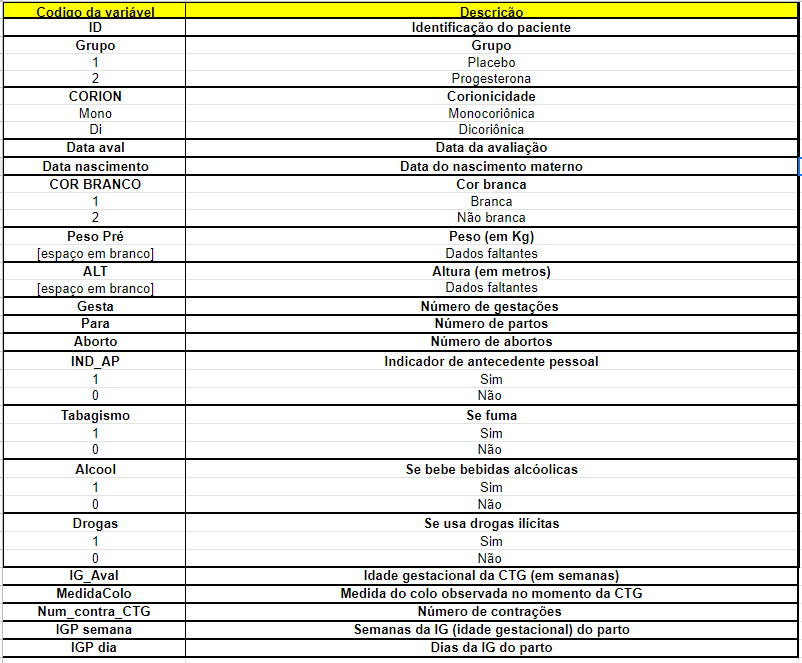
\includegraphics[width=1\linewidth]{figures/dicionario_dados_progest} \caption{Variáveis da base de dados gestações gemelares.}\label{fig:dic1}
\end{figure}

A seguir está o exemplo de como os dados de 5 indivíduos estão tabulados.

\begin{tabular}{r|r|l|l|l|r|l|l|r|r|r|r|r|r|r|r|r|r|r|r|l}
\hline
ID & Grupo & CORION & Data aval & Data nascimento & COR BRANCO & Peso Pré & ALT & Gesta & Para & Aborto & IND\_AP & Tabagismo & Alcool & Drogas & IG\_Aval & MedidaColo & Num\_contra\_CTG & IGP semana & IGP dia & oi\\
\hline
18 & 2 & Di & 2016-03-21 & 1987-03-29 & 1 & 80.0 & 1.59 & 1 & 0 & 0 & 1 & 0 & 0 & 0 & 31.43 & 20.00 & 7 & 37 & 5 & NA\\
\hline
19 & 2 & Di & 2016-02-17 & 1980-02-26 & 1 & NA & 1.62 & 4 & 3 & 0 & 0 & 1 & 1 & 0 & 27.00 & 6.60 & 2 & 33 & 2 & NA\\
\hline
20 & 1 & Di & 2017-12-14 & 1998-12-19 & 2 & 61.0 & 1.64 & 1 & 0 & 0 & 0 & 0 & 0 & 0 & 33.71 & 7.00 & 10 & 35 & 3 & NA\\
\hline
21 & 1 & Mono & 2017-04-23 & 1988-04-30 & 1 & 44.0 & 1.64 & 1 & 0 & 0 & 0 & 0 & 0 & 0 & 83.86 & 5.83 & 8 & 36 & 3 & NA\\
\hline
22 & 2 & Di & 2016-03-21 & 1995-03-27 & 2 & 100.0 & 1.59 & 2 & 1 & 0 & 1 & 0 & 1 & 0 & 33.71 & 12.10 & 3 & 37 & 6 & NA\\
\hline
\end{tabular}

Essa base de dados está disponível em \url{https://daslab-ufes.github.io/materiais/}, chamado de ``Dados gemelares''.

\hypertarget{gestauxe7uxf5es-gemelares---depressuxe3o-e-amamentauxe7uxe3o}{%
\subsection{Gestações gemelares - depressão e amamentação}\label{gestauxe7uxf5es-gemelares---depressuxe3o-e-amamentauxe7uxe3o}}

Esta base de dados fictícia apresenta informações sobre depressão e amamentação das mesmas observações consideradas na base de dados Gestações gemelares, apresentada no item anterior.

O questionário de depressão EDPS foi respondido pelas gestantes no primeiro trimestre gestacional e respondido novamente pelas mesmas gestantes no quarto mês pós-parto. Esse questionário retorna um escore (de 0 a 30 pontos), em que quanto maior seu valor, maior indicador de depressão.

Sobre a amamentação, foram divididos três grupos a depender das orientações sobre a amamentação recebidas durante o pré-natal. O grupo 1 é formado pelas gestantes que tiveram mentorias durante o pré-natal e acompanhamento nas amamentações das primeiras semanas; o grupo 2 é formado pelas gestações que receberam apenas orientações durante o pré-natal e no grupo 3 estão as gestantes que não receberam orientações sobre amamentação.

São as características observadas:

\begin{figure}
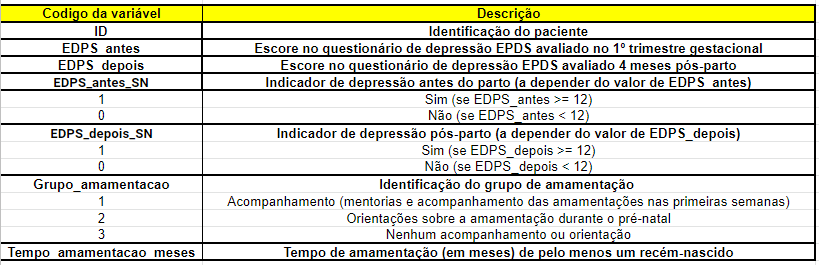
\includegraphics[width=1\linewidth]{figures/dicionario_dados_progest2} \caption{Variáveis da base de dados gestações gemelares - depressão e amamentação.}\label{fig:dic2}
\end{figure}

A seguir está o exemplo de como os dados de 5 indivíduos estão tabulados.

\begin{tabular}{r|r|r|r|r|r|r}
\hline
ID & EPDS\_antes & EPDS\_depois & EDPS\_antes\_SN & EDPS\_depois\_SN & Grupo\_amamentacao & Tempo\_amamentacao\_meses\\
\hline
18 & 2 & 1 & 0 & 0 & 1 & 10\\
\hline
19 & 6 & 3 & 0 & 0 & 2 & 4\\
\hline
20 & 10 & 8 & 0 & 0 & 2 & 15\\
\hline
21 & 15 & 18 & 1 & 1 & 2 & 11\\
\hline
22 & 3 & 4 & 0 & 0 & 2 & 8\\
\hline
\end{tabular}

Essa base de dados está disponível em \url{https://daslab-ufes.github.io/materiais/}, chamado de ``Dados gemelares - depressão e amamentação''.

\hypertarget{sobre-o-software-r}{%
\section{Sobre o software R}\label{sobre-o-software-r}}

R é um ambiente computacional e uma linguagem de programação para manipulação, análise e visualização de dados. É considerado um dos melhores ambiente computacional para essa finalidade. O R é mantido pela \href{https://cran.r-project.org/}{R Development Core Team} e está disponível para diferentes sistemas operacionais: Linux, Mac e Windows.

O software é livre, ou seja, gratuito, com código aberto em uma linguagem acessível. Nele estão implementadas muitas metodologias estatísticas. Muitas destas fazem parte do ambiente base de R e outras acompanham o ambiente sob a forma de pacotes, o que torna o R altamente expansível. Os pacotes são bibliotecas com dados e funções para diferentes áreas do conhecimento relacionado a estatística e áreas afins, devidamente documentados.

O R possui uma comunidade extremamente ativa, engajada desde o aprimoramento de ferramentas e desenvolvimento de novas bibliotecas, até o suporte aos usuários. Sobre o desenvolvimento de novas bibliotecas, um pesquisador em Estatística que desenvolve um novo modelo estatístico pode disponibilizar o seu modelo em um pacote acessível a que se interessam pelo modelo.

Além disso, a disponibilidade e compartilhamento da pesquisa em um pacote no R é uma boa prática quando falamos de reprodutibilidade na Ciência. Ainda nesse ponto, realizar as análises de uma pesquisa aplicada em um programa livre e acessível a todos é um dos principais pontos para permitir reprodutibilidade.

Ao optar por programar em R também implica na escolha de uma IDE (Integrated Development Environment) que, na grande maioria dos casos, será o \href{https://rstudio.com}{RStudio}. O RStudio é um conjunto de ferramentas integradas projetadas para editar e executar os códigos em R. Assim, quando for o interesse utilizar o R, só precisa abrir o RStudio (R é automaticamente carregado).

Para instalação do R e do RStudio, veja a Seção que segue.

\hypertarget{instalauxe7uxe3o-r-e-rstudio}{%
\section{Instalação R e RStudio}\label{instalauxe7uxe3o-r-e-rstudio}}

\hypertarget{instalauxe7uxe3o-r}{%
\subsection{Instalação R}\label{instalauxe7uxe3o-r}}

Nessa Seção, vamos apresentar como instalar o R e o RStudio para os três sistemas operacionais: Windows, MAC e Linux, respectivamente.

\hypertarget{para-windows}{%
\subsubsection{Para Windows}\label{para-windows}}

Os passos para instalar o R quando o sistema operacional é Windows são os seguintes:

\begin{enumerate}
\def\labelenumi{\arabic{enumi})}
\tightlist
\item
  Entre neste \href{https://cran.r-project.org/bin/windows/base/}{link} para acessar a página do R e clique em Download, como no link destacado em retângulo vermelho na Figura \ref{fig:windows1}. Note que o 3.6.1 é o número da versão mais recente disponível no momento da construção desse material (5/7/19).
\end{enumerate}

\begin{figure}
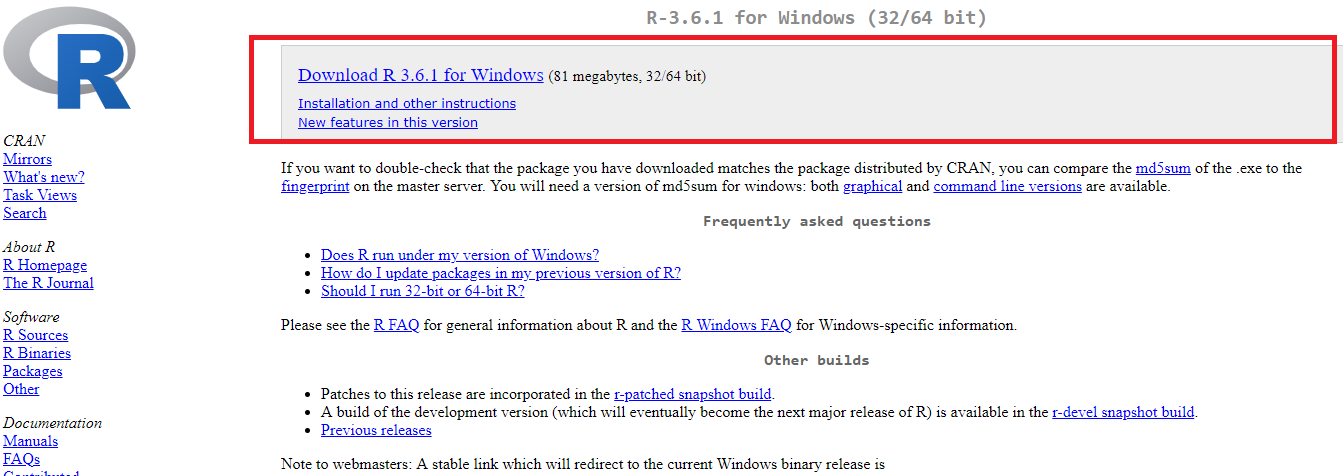
\includegraphics[width=1\linewidth]{figures/install_Windows} \caption{Download R para Windows}\label{fig:windows1}
\end{figure}

\begin{enumerate}
\def\labelenumi{\arabic{enumi})}
\setcounter{enumi}{1}
\tightlist
\item
  Salve o arquivo de instalação em algum caminho de interesse do seu computador. Por exemplo, na Figura \ref{fig:windows2} mostra que a pasta é ``Downloads''.
\end{enumerate}

\begin{figure}
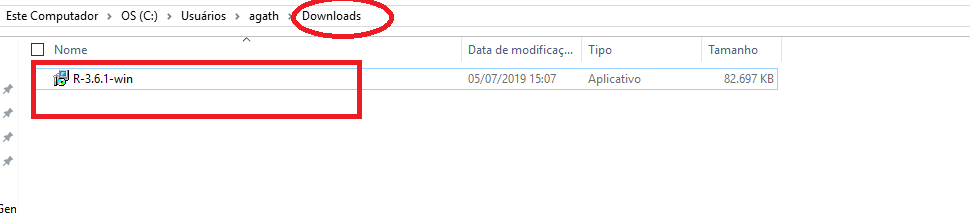
\includegraphics[width=1\linewidth]{figures/install_Windows2} \caption{Instalador}\label{fig:windows2}
\end{figure}

\begin{enumerate}
\def\labelenumi{\arabic{enumi})}
\setcounter{enumi}{2}
\tightlist
\item
  Clique duas vezes com o botão esquerdo no instalador para iniciar a instalação. O próximo passo é escolher a lingua para instalação. Na Figura \ref{fig:windows3} abaixo é português.
\end{enumerate}

\begin{figure}
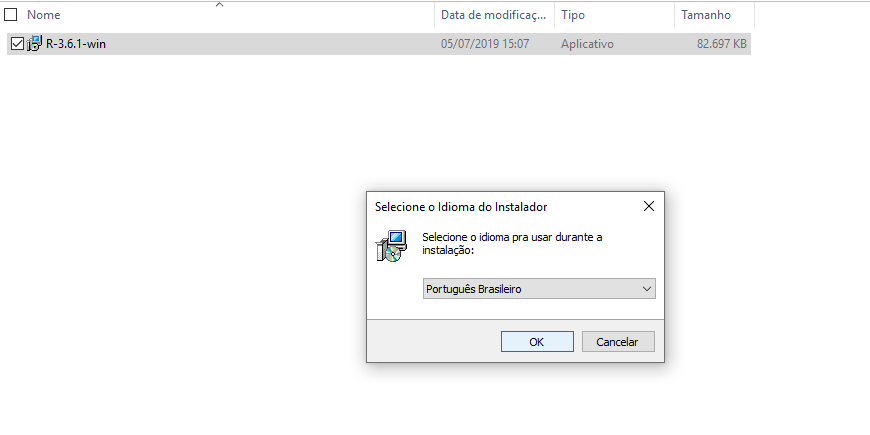
\includegraphics[width=1\linewidth]{figures/install_Windows3} \caption{Escolha da lingua para instalação}\label{fig:windows3}
\end{figure}

\begin{enumerate}
\def\labelenumi{\arabic{enumi})}
\setcounter{enumi}{3}
\tightlist
\item
  Clique em ``Próximo'' nas próximas janelas, como nas Figuras \ref{fig:windows4} a \ref{fig:windows9}.
\end{enumerate}

\begin{figure}
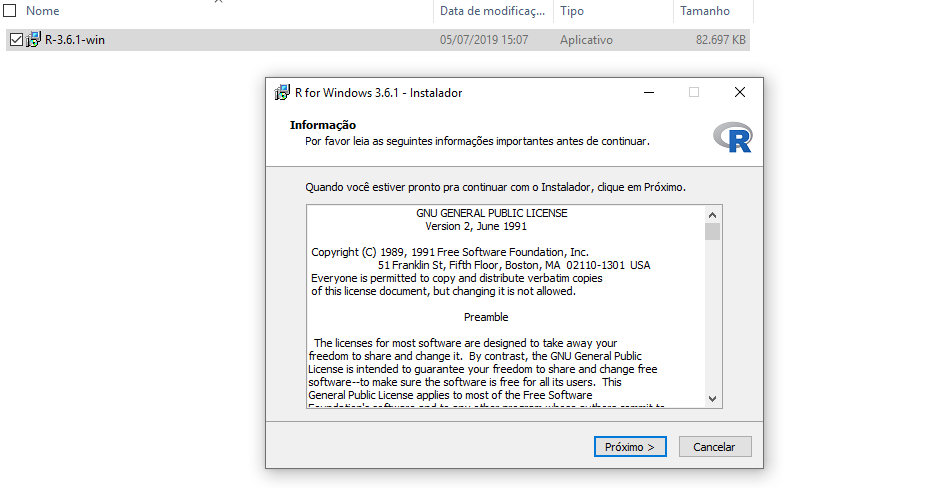
\includegraphics[width=1\linewidth]{figures/install_Windows4} \caption{Próximo }\label{fig:windows4}
\end{figure}

\begin{figure}
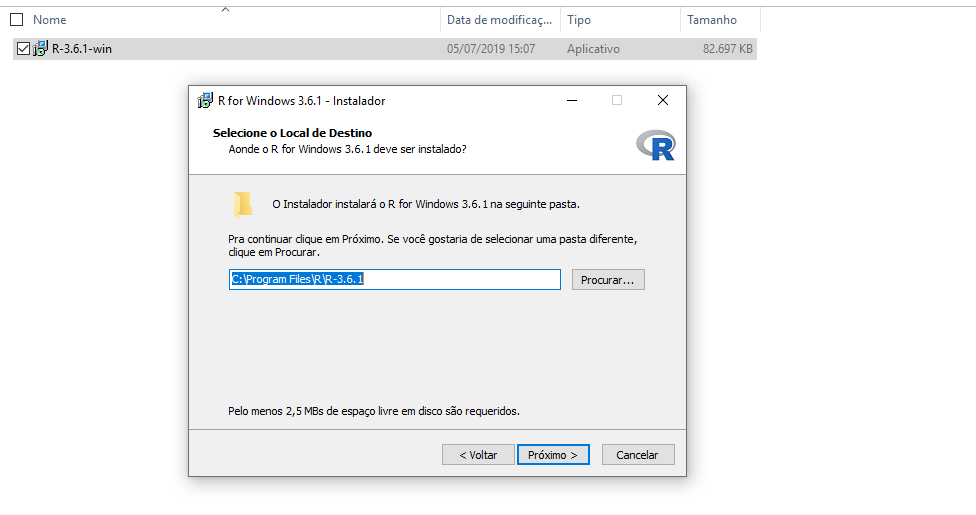
\includegraphics[width=1\linewidth]{figures/install_Windows5} \caption{\label{fig:windows5}Próximo }\label{fig:windows5}
\end{figure}

\begin{figure}
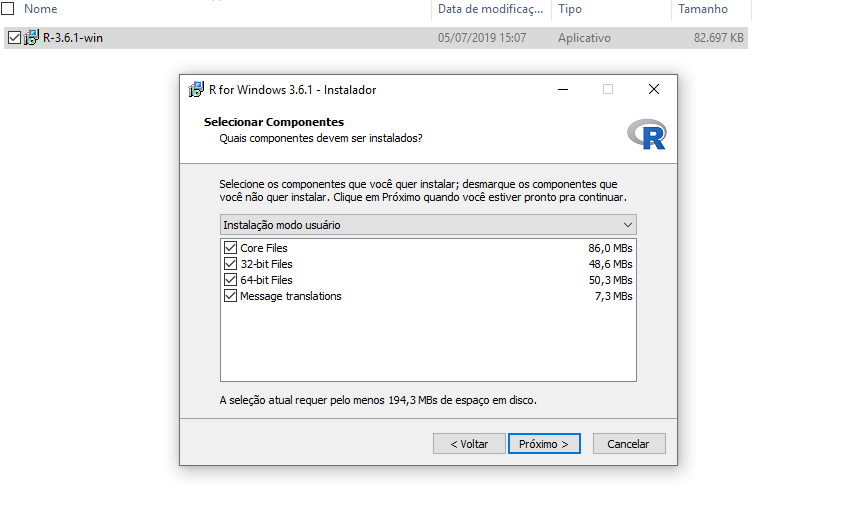
\includegraphics[width=1\linewidth]{figures/install_Windows6} \caption{\label{fig:windows6}Próximo }\label{fig:windows6}
\end{figure}

\begin{figure}
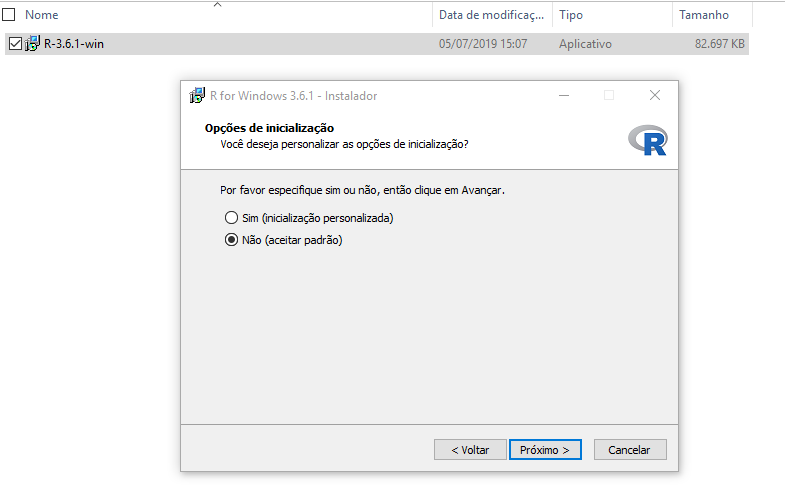
\includegraphics[width=1\linewidth]{figures/install_Windows7} \caption{\label{fig:windows7}Próximo }\label{fig:windows7}
\end{figure}

\begin{figure}
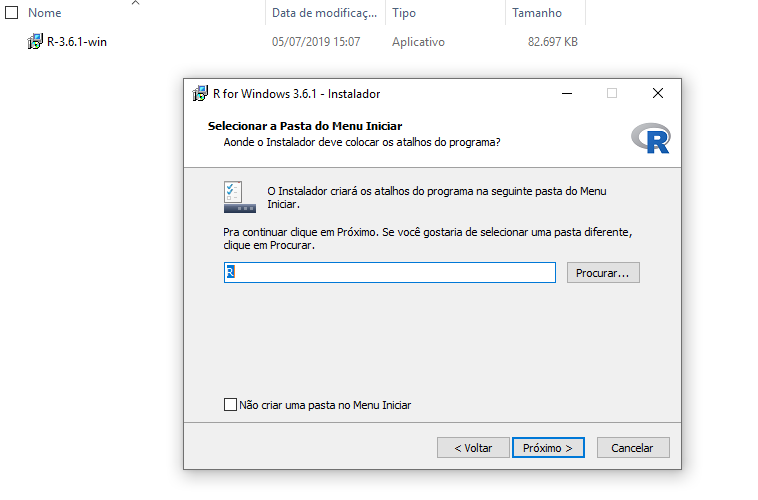
\includegraphics[width=1\linewidth]{figures/install_Windows8} \caption{\label{fig:windows8}Próximo }\label{fig:windows8}
\end{figure}

\begin{figure}
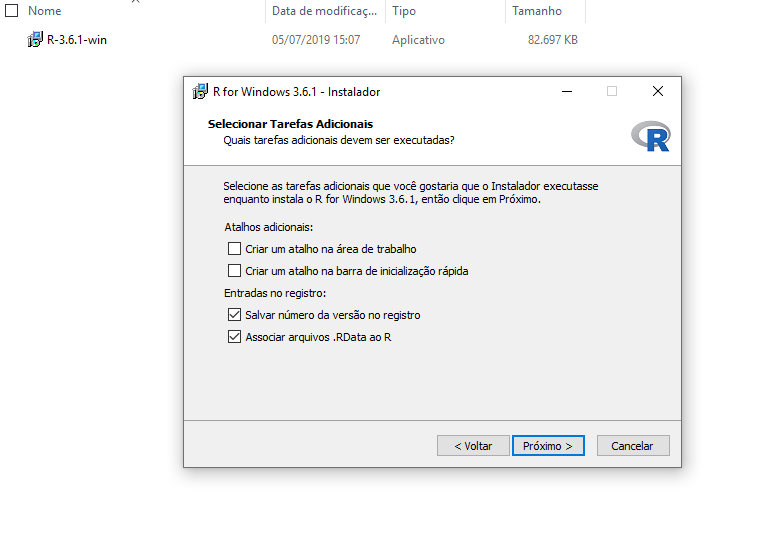
\includegraphics[width=1\linewidth]{figures/install_Windows9} \caption{\label{fig:windows9}Próximo }\label{fig:windows9}
\end{figure}

\begin{enumerate}
\def\labelenumi{\arabic{enumi})}
\setcounter{enumi}{4}
\tightlist
\item
  Pronto, agora o software R será instalado, como na Figura \ref{fig:windows10}, e quando terminar, aparecerá uma janela como apresentado na Figura \ref{fig:windows11}.
\end{enumerate}

\begin{figure}
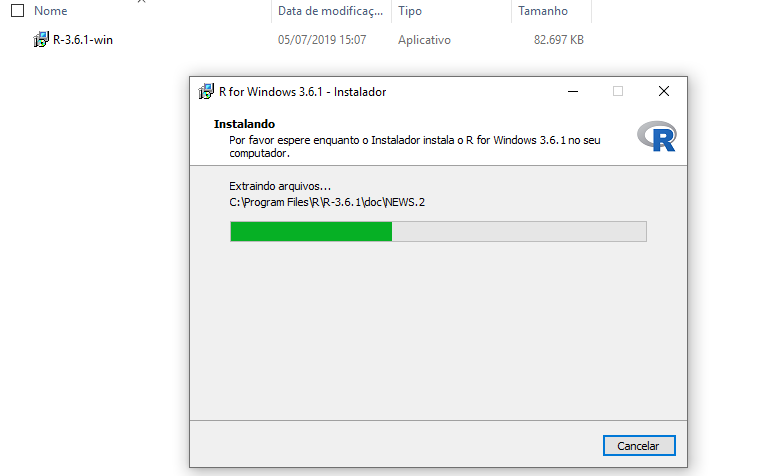
\includegraphics[width=1\linewidth]{figures/install_Windows10} \caption{\label{fig:windows10}Instalação do R}\label{fig:windows10}
\end{figure}

\begin{figure}
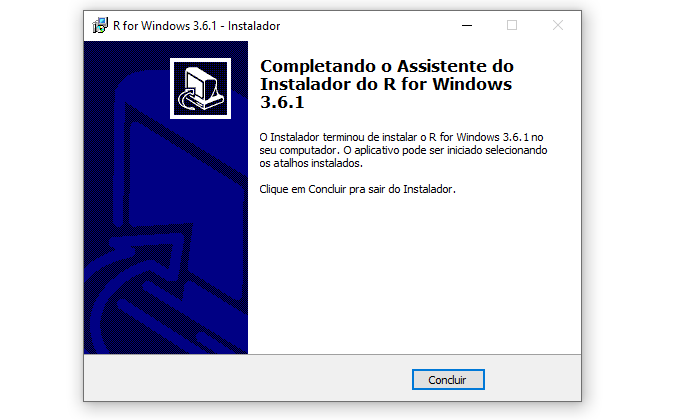
\includegraphics[width=1\linewidth]{figures/install_Windows11} \caption{\label{fig:windows11}Pronto: R instalado}\label{fig:windows11}
\end{figure}

\hypertarget{para-mac}{%
\subsubsection{Para MAC}\label{para-mac}}

Os passos para instalar o R quando o sistema operacional é OS X (Mac) são os seguintes:

\begin{enumerate}
\def\labelenumi{\arabic{enumi})}
\tightlist
\item
  Entre no \href{https://cran.r-project.org}{site} e clique em Download R for (MAC) OS X, conforme destacado abaixo em retângulo vermelho na Figura \ref{fig:mac1}.
\end{enumerate}

\begin{figure}
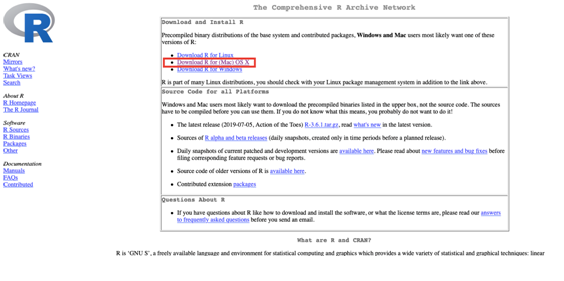
\includegraphics[width=1\linewidth]{figures/mac_R_1} \caption{\label{fig:mac1} Download R para Mac}\label{fig:mac1}
\end{figure}

\begin{enumerate}
\def\labelenumi{\arabic{enumi})}
\setcounter{enumi}{1}
\tightlist
\item
  Baixe o pacote R-3.6.1.pkg clicando no link indicado no retângulo vermelho na Figura \ref{fig:mac2}. Note que o 3.6.1 é o número da versão mais recente disponível no momento da confecção desse material.
\end{enumerate}

\begin{figure}
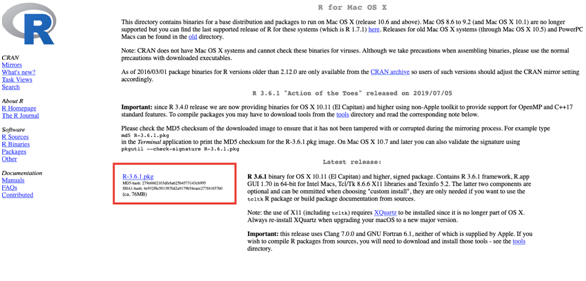
\includegraphics[width=1\linewidth]{figures/mac_R_2} \caption{\label{fig:mac2} Download R para Mac }\label{fig:mac2}
\end{figure}

\begin{enumerate}
\def\labelenumi{\arabic{enumi})}
\setcounter{enumi}{2}
\tightlist
\item
  Caso você não tenha configurado a pasta de descargas, o pacote será baixado na pasta ``Downloads'', como mostrado na seguinte Figura \ref{fig:mac3}. Observe que dois arquivos são baixados, clique duas vezes no arquivo ``R-3.6.1.pkg'' para abrir o assistente de instalação que o guiará durante o processo.
\end{enumerate}

\begin{figure}
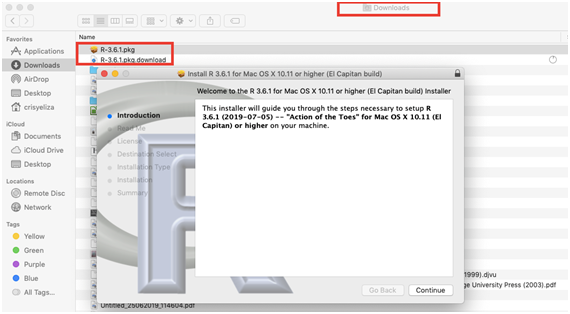
\includegraphics[width=1\linewidth]{figures/mac_R_3} \caption{\label{fig:mac3} Pasta para instalação}\label{fig:mac3}
\end{figure}

\begin{enumerate}
\def\labelenumi{\arabic{enumi})}
\setcounter{enumi}{3}
\tightlist
\item
  Acompanhe os passos indicados pelo instalador (Figura \ref{fig:mac4}).
\end{enumerate}

\begin{figure}
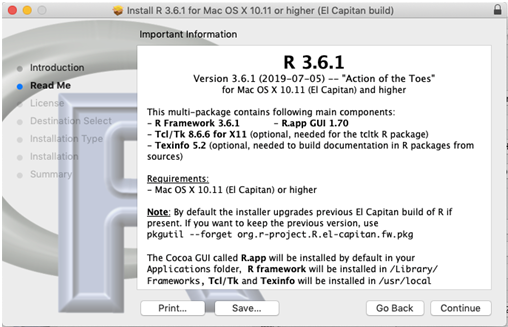
\includegraphics[width=1\linewidth]{figures/mac_R_4} \caption{\label{fig:mac4} Instalação}\label{fig:mac4}
\end{figure}

\begin{enumerate}
\def\labelenumi{\arabic{enumi})}
\setcounter{enumi}{4}
\tightlist
\item
  Deve concordar com os termos da licença, clique em ``Agree'' (Figura \ref{fig:mac5}).

  \begin{figure}
  
\includegraphics[width=1\linewidth]{figures/mac_R_5} \caption{\label{fig:mac5} Instalação}\label{fig:mac5}
  \end{figure}
\item
  Selecione o lugar onde instalará o programa, no caso de ter o disco particionado e assim desejar instalar em uma parte específica. Caso contrário, continue (Figura \ref{fig:mac6} e \ref{fig:mac7}).
\end{enumerate}

\begin{figure}
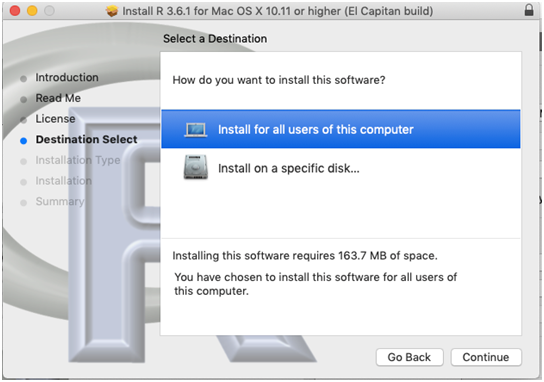
\includegraphics[width=1\linewidth]{figures/mac_R_6} \caption{\label{fig:mac6} Instalação}\label{fig:mac6}
\end{figure}

\begin{figure}
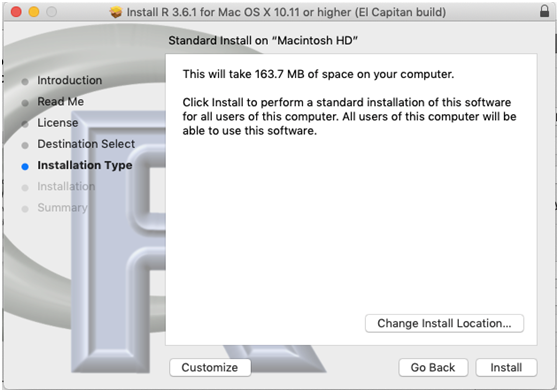
\includegraphics[width=1\linewidth]{figures/mac_R_7} \caption{\label{fig:mac7} Instalação}\label{fig:mac7}
\end{figure}

\begin{enumerate}
\def\labelenumi{\arabic{enumi})}
\setcounter{enumi}{6}
\tightlist
\item
  Para finalizar a instalação, o assistente lhe pedirá nome de usuário e senha do seu notebook, como apresentado na Figura \ref{fig:mac8}.
\end{enumerate}

\begin{figure}
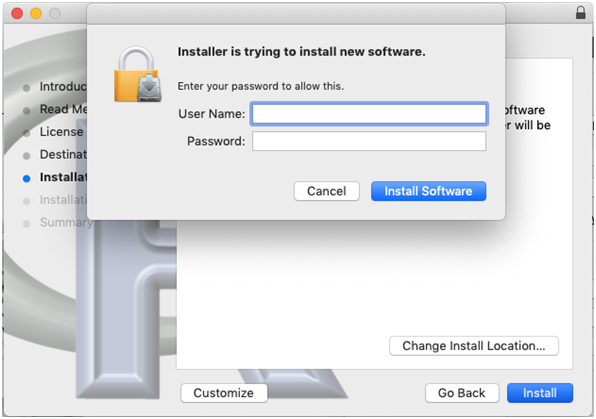
\includegraphics[width=1\linewidth]{figures/mac_R_8} \caption{\label{fig:mac8} Instalação}\label{fig:mac8}
\end{figure}

\begin{enumerate}
\def\labelenumi{\arabic{enumi})}
\setcounter{enumi}{7}
\tightlist
\item
  Pronto, agora o software R será instalado, como na Figura \ref{fig:mac9}, e quando terminar, aparecerá uma janela como apresentado na Figura \ref{fig:mac10}.
\end{enumerate}

\begin{figure}
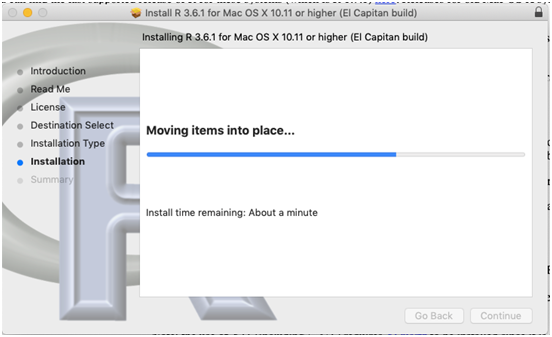
\includegraphics[width=1\linewidth]{figures/mac_R_9} \caption{\label{fig:mac9} Instalação}\label{fig:mac9}
\end{figure}

\begin{figure}

\includegraphics[width=1\linewidth]{figures/mac_R_10} \caption{\label{fig:mac10} Instalação}\label{fig:mac10}
\end{figure}

\hypertarget{para-linux}{%
\subsubsection{Para Linux}\label{para-linux}}

A instalação do R no Linux depende da distribuição utilizada. Entre neste \href{https://cran.r-project.org/}{link} para acessar a página do R e clique em Download R for Linux, como no link destacado em retângulo vermelho na Figura \ref{fig:linux1}. Em seguida, clique no link referente à distribuição utilizada (Figura \ref{fig:linux2}).

\begin{figure}

\includegraphics[width=1\linewidth]{figures/install_R_linux} \caption{\label{fig:linux1}Download em Linux}\label{fig:linux1}
\end{figure}

\begin{figure}
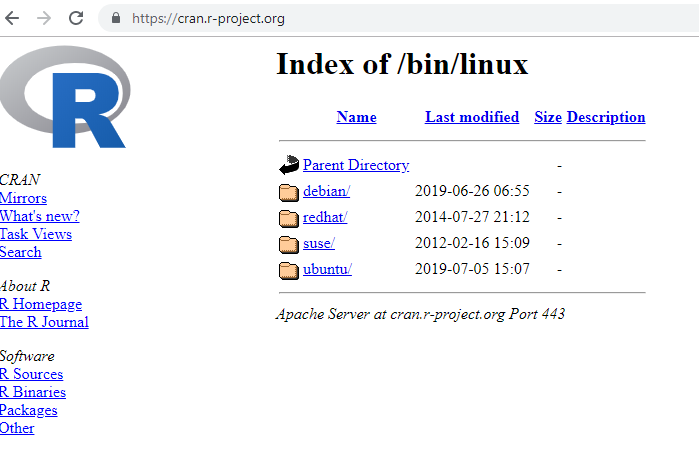
\includegraphics[width=1\linewidth]{figures/install_R_linux2} \caption{\label{fig:linux2}Download em Linux}\label{fig:linux2}
\end{figure}

\hypertarget{instalauxe7uxe3o-rstudio}{%
\subsection{Instalação RStudio}\label{instalauxe7uxe3o-rstudio}}

O RStudio é um conjunto de ferramentas integradas projetadas (IDE - Integrated Development Environment) da linguagem R para auxiliar na produtividade ao utilizar o R.

\hypertarget{para-windows-1}{%
\subsubsection{Para Windows}\label{para-windows-1}}

\begin{enumerate}
\def\labelenumi{\arabic{enumi})}
\tightlist
\item
  Entre neste \href{https://www.rstudio.com/products/rstudio/download/}{link} e clique em Download como em destaque na Figura \ref{fig:rswindows1}.
\end{enumerate}

\begin{figure}
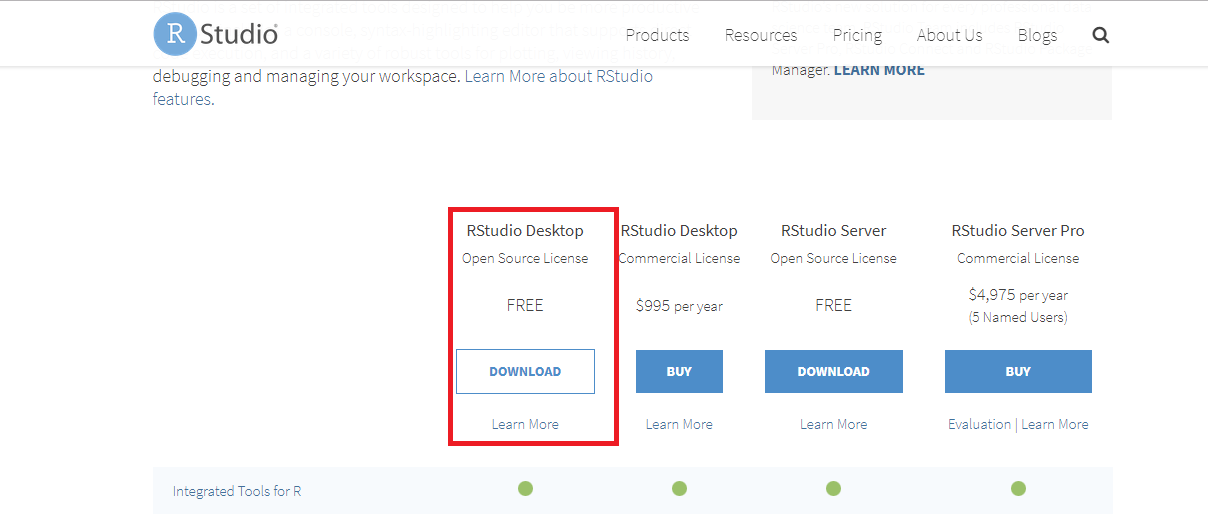
\includegraphics[width=1\linewidth]{figures/install_Rstudio1} \caption{\label{fig:rswindows1}Site para download do RStudio}\label{fig:rswindows1}
\end{figure}

\begin{enumerate}
\def\labelenumi{\arabic{enumi})}
\setcounter{enumi}{1}
\tightlist
\item
  Clique no instalador em destaque na Figura \ref{fig:rswindows2}.
\end{enumerate}

\begin{figure}
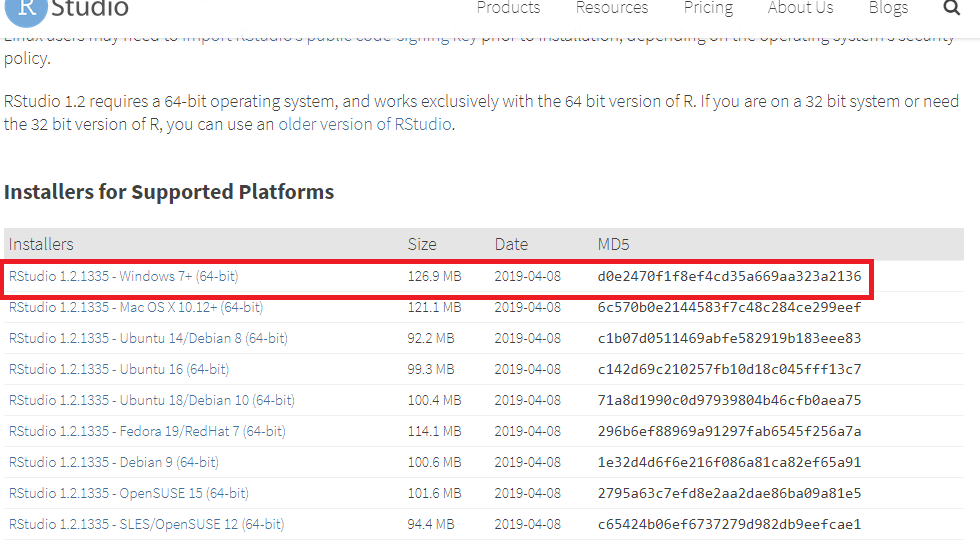
\includegraphics[width=1\linewidth]{figures/install_Rstudio2} \caption{\label{fig:rswindows2}Link para download do RStudio}\label{fig:rswindows2}
\end{figure}

\begin{enumerate}
\def\labelenumi{\arabic{enumi})}
\setcounter{enumi}{2}
\tightlist
\item
  Ao clicar no link, será feito o download do instalador e salvo na pasta de interesse. No caso da Figura \ref{fig:rswindows3}, o instalador está na pasta Downloads. Dê dois cliques no botão esquerdo no arquivo para iniciar o download do arquivo.
\end{enumerate}

\begin{figure}
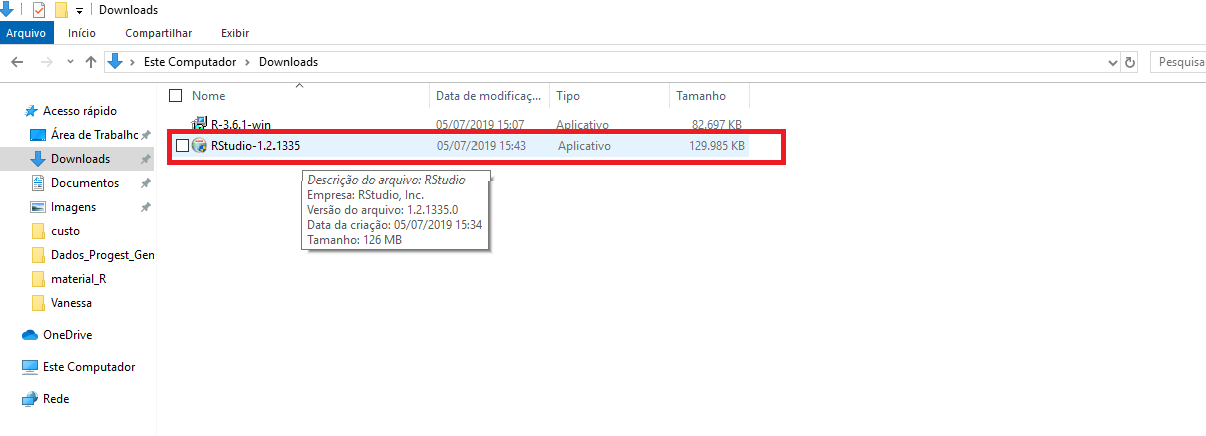
\includegraphics[width=1\linewidth]{figures/install_Rstudio3} \caption{\label{fig:rswindows3} Instalador}\label{fig:rswindows3}
\end{figure}

\begin{enumerate}
\def\labelenumi{\arabic{enumi})}
\setcounter{enumi}{3}
\tightlist
\item
  Clique em ``Próximo'' nas próximas janelas e na última ``Instalar'', como nas Figuras \ref{fig:rswindows4} a \ref{fig:rswindows6}.
\end{enumerate}

\begin{figure}
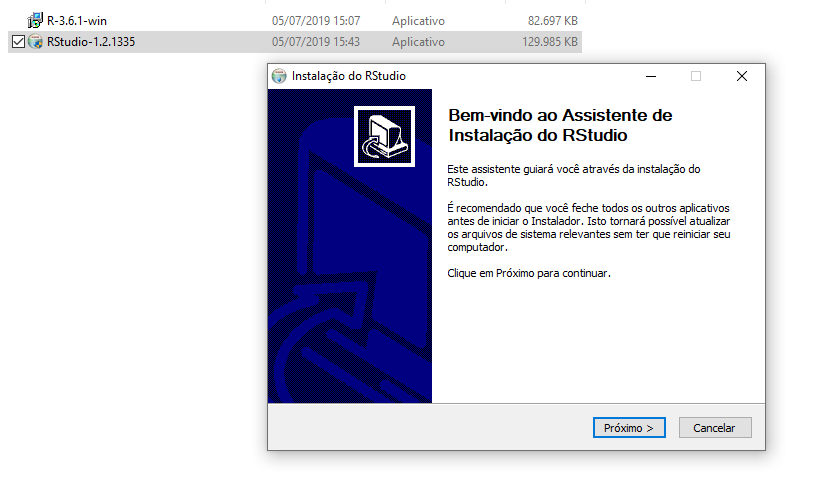
\includegraphics[width=1\linewidth]{figures/install_Rstudio4} \caption{\label{fig:rswindows4} Instalação}\label{fig:rswindows4}
\end{figure}

\begin{figure}
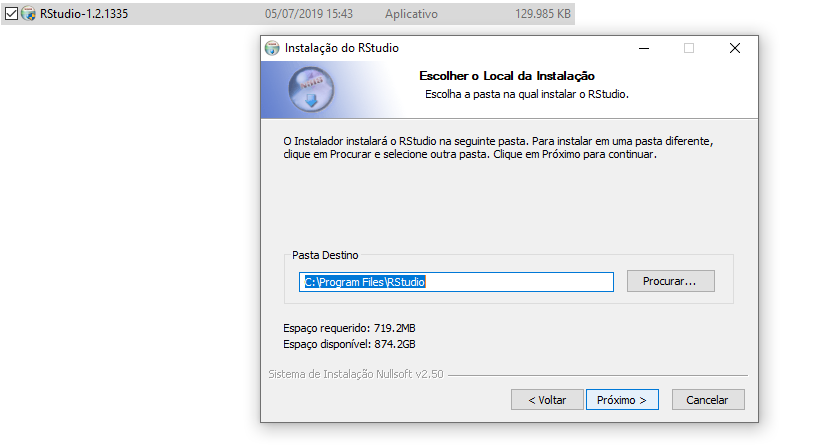
\includegraphics[width=1\linewidth]{figures/install_Rstudio5} \caption{\label{fig:rswindows5} Instalação}\label{fig:rswindows5}
\end{figure}

\begin{figure}
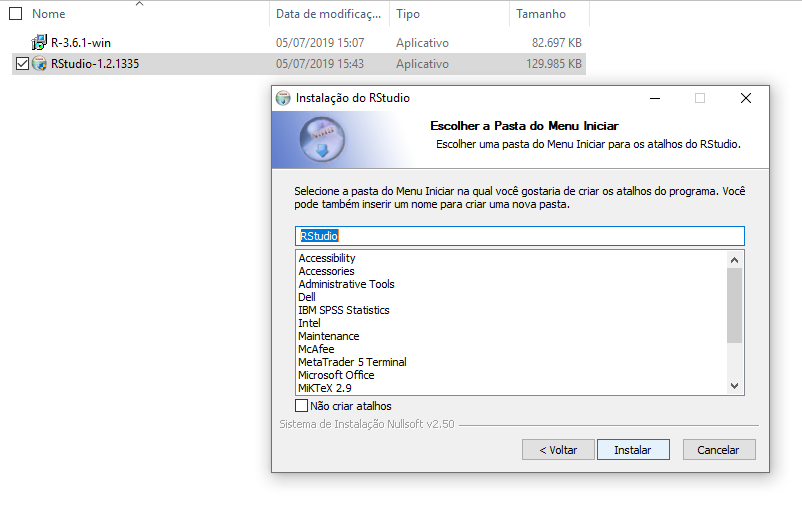
\includegraphics[width=1\linewidth]{figures/install_Rstudio6} \caption{\label{fig:rswindows6} Instalação}\label{fig:rswindows6}
\end{figure}

\begin{enumerate}
\def\labelenumi{\arabic{enumi})}
\setcounter{enumi}{4}
\tightlist
\item
  Pronto, a instalação será iniciada, como na Figura \ref{fig:rswindows7}.
\end{enumerate}

\begin{figure}
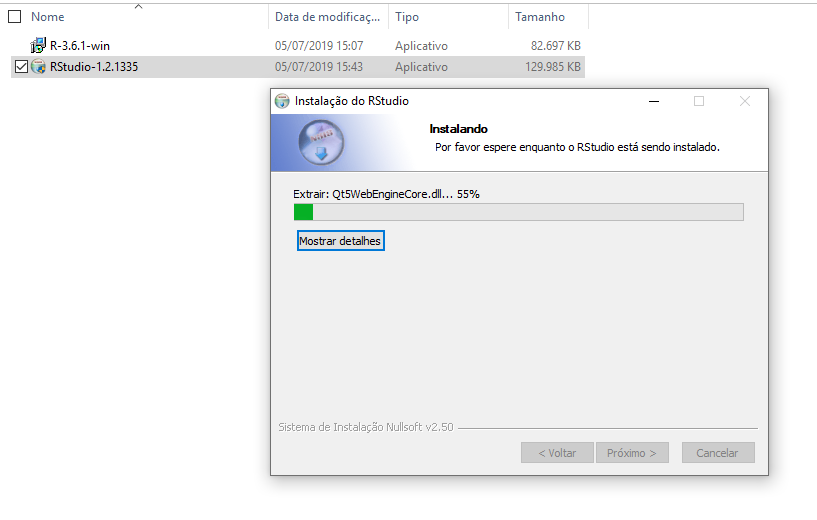
\includegraphics[width=1\linewidth]{figures/install_Rstudio7} \caption{\label{fig:rswindows7} Instalação}\label{fig:rswindows7}
\end{figure}

\hypertarget{para-mac-1}{%
\subsubsection{Para MAC}\label{para-mac-1}}

\begin{enumerate}
\def\labelenumi{\arabic{enumi})}
\tightlist
\item
  Entre neste \href{https://www.rstudio.com/products/rstudio/download/}{link} e clique em Download como em destaque na Figura \ref{fig:rsmac1}.
\end{enumerate}

\begin{figure}
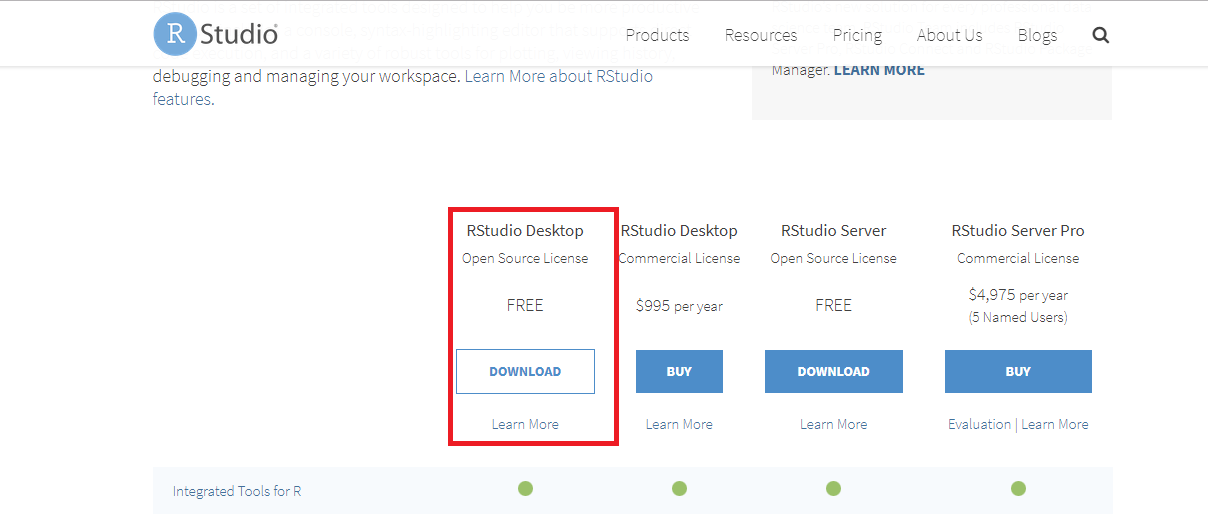
\includegraphics[width=1\linewidth]{figures/install_Rstudio1} \caption{\label{fig:rsmac1}Site para download do RStudio}\label{fig:rsmac1}
\end{figure}

\begin{enumerate}
\def\labelenumi{\arabic{enumi})}
\setcounter{enumi}{1}
\tightlist
\item
  Clique no instalador como destacado na Figura \ref{fig:rsmac2}.
\end{enumerate}

\begin{figure}
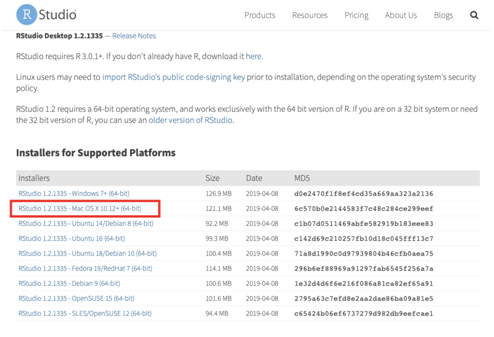
\includegraphics[width=1\linewidth]{figures/mac_RSt_1} \caption{\label{fig:rsmac2}Site para download do RStudio para Mac}\label{fig:rsmac2}
\end{figure}

\begin{enumerate}
\def\labelenumi{\arabic{enumi})}
\setcounter{enumi}{2}
\tightlist
\item
  Ao clicar no link, será feito o download do instalador e salvo na pasta de interesse. Caso você não tenha configurado a pasta de descargas, o instalador ficará na pasta ``Downloads'', como na Figura \ref{fig:rsmac3}.
\end{enumerate}

\begin{figure}
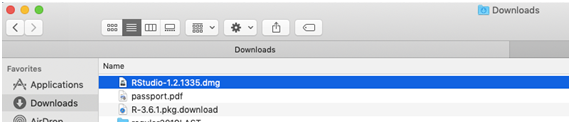
\includegraphics[width=1\linewidth]{figures/mac_RSt_2} \caption{\label{fig:rsmac3} Instalador salvo em pasta}\label{fig:rsmac3}
\end{figure}

\begin{enumerate}
\def\labelenumi{\arabic{enumi})}
\setcounter{enumi}{3}
\tightlist
\item
  Clicando duas vezes no arquivo ``RStudio-1.2.1335.dmg'' (versãos mais atual do RStudio), será feita a descarga do mesmo abrindo a janela conforme na Figura \ref{fig:rsmac4}. Clique no aplicativo de RStudio destacado em vermelho também na Figura \ref{fig:rsmac4}.
\end{enumerate}

\begin{figure}
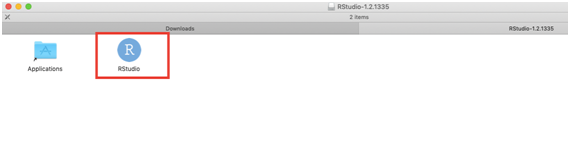
\includegraphics[width=1\linewidth]{figures/mac_RSt_3} \caption{\label{fig:rsmac4} Instalação}\label{fig:rsmac4}
\end{figure}

\begin{enumerate}
\def\labelenumi{\arabic{enumi})}
\setcounter{enumi}{4}
\tightlist
\item
  O instalador pode perguntar se está seguro que o aplicativo será baixado da internet e clique em ``Open'' (Figura \ref{fig:rsmac5}).
\end{enumerate}

\begin{figure}
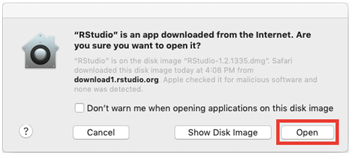
\includegraphics[width=1\linewidth]{figures/mac_RSt_4} \caption{\label{fig:rsmac5} Instalação}\label{fig:rsmac5}
\end{figure}

\begin{enumerate}
\def\labelenumi{\arabic{enumi})}
\setcounter{enumi}{5}
\tightlist
\item
  Pronto! Imediatamente abre o RStudio, como na Figura \ref{fig:rsmac6}, e você já pode utilizar.
\end{enumerate}

\begin{figure}
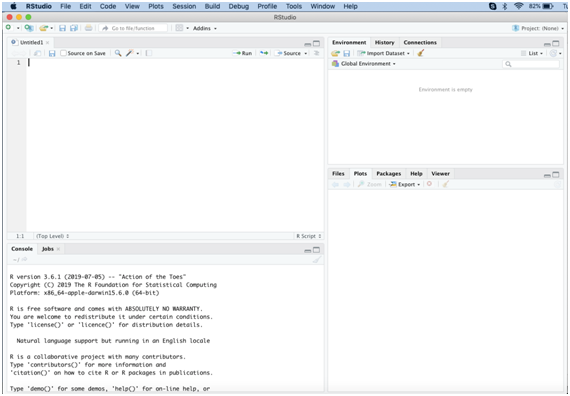
\includegraphics[width=1\linewidth]{figures/mac_RSt_5} \caption{\label{fig:rsmac6} Instalação}\label{fig:rsmac6}
\end{figure}

\hypertarget{para-linux-1}{%
\subsubsection{Para Linux}\label{para-linux-1}}

\begin{enumerate}
\def\labelenumi{\arabic{enumi})}
\tightlist
\item
  Entre neste \href{https://www.rstudio.com/products/rstudio/download/}{link} e clique em Download como em destaque na Figura \ref{fig:rslinux1}.
\end{enumerate}

\begin{figure}
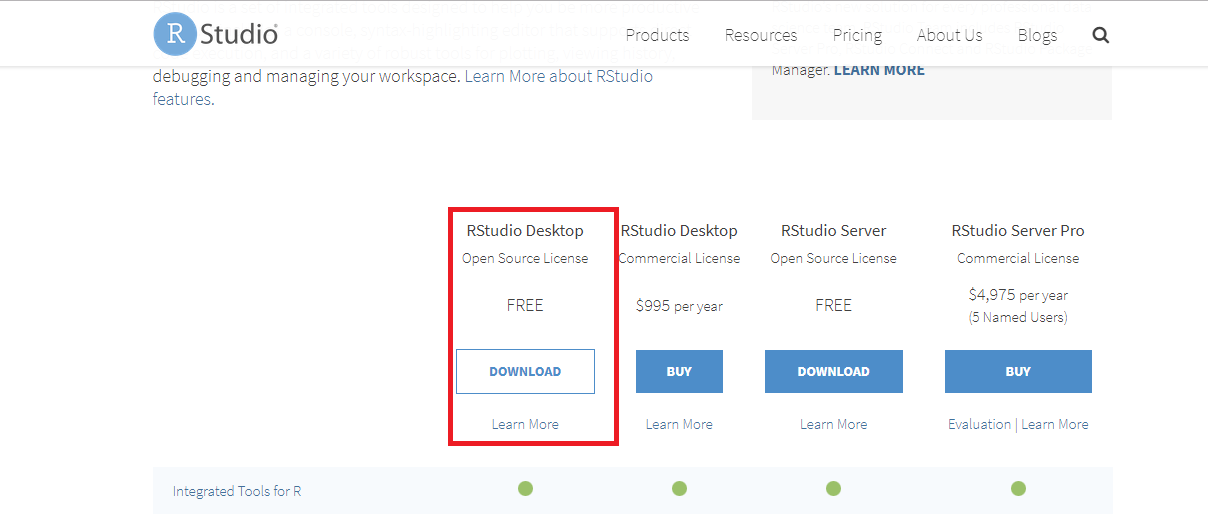
\includegraphics[width=1\linewidth]{figures/install_Rstudio1} \caption{\label{fig:rslinux1}Site para download do RStudio}\label{fig:rslinux1}
\end{figure}

\begin{enumerate}
\def\labelenumi{\arabic{enumi})}
\setcounter{enumi}{1}
\tightlist
\item
  Clique no link referente à distribuição utilizada (Figura \ref{fig:rslinux2}).

  \begin{figure}
  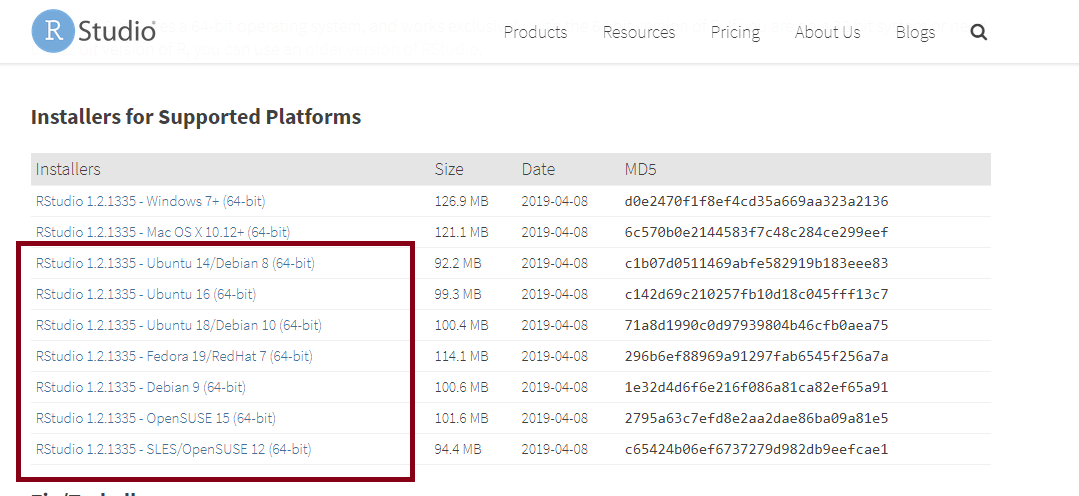
\includegraphics[width=1\linewidth]{figures/install_Rstudio_linux} \caption{\label{fig:rslinux2} Download do RStudio}\label{fig:rslinux2}
  \end{figure}
\end{enumerate}

\hypertarget{primeiros-passos-com-r-e-rstudio.}{%
\section{Primeiros passos com R e RStudio.}\label{primeiros-passos-com-r-e-rstudio.}}

\hypertarget{primeiros-contatos-com-rstudio}{%
\subsection{Primeiros contatos com RStudio}\label{primeiros-contatos-com-rstudio}}

O RStudio é um conjunto de ferramentas integradas projetadas (IDE - Integrated Development Environment) da linguagem R para editar e executar os códigos em R.

Tem quatro áreas, conforme a Figura \ref{fig:telarstudio1}.

\begin{figure}
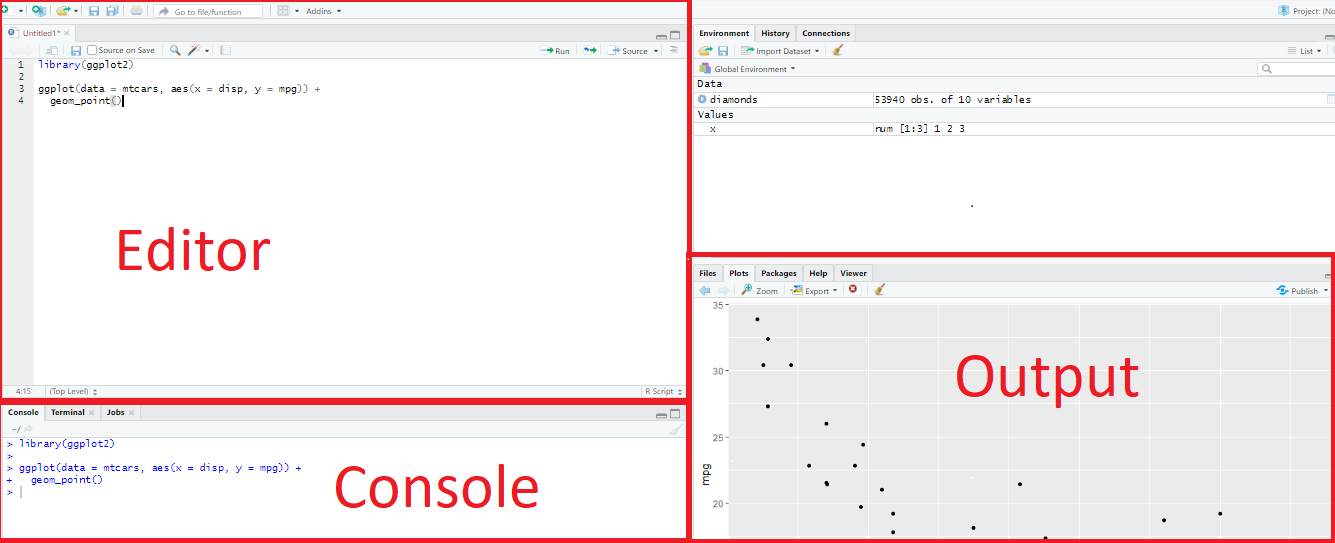
\includegraphics[width=1\linewidth]{figures/rstudio1} \caption{\label{fig:rstudio1} Visualização do RStudio}\label{fig:telarstudio1}
\end{figure}

A seguir descrevemos melhor os painéis e abas do RStudio:

\begin{itemize}
\item
  Editor/Scripts: É onde escrever os códigos. Arquivos do tipo .R.
\item
  Console: Executar os comandos e ver os resultados.
\item
  Enviroment: Painel com todos os objetos criados.
\item
  History: História dos comandos executados.
\item
  Files: Navegar em pastas e arquivos.
\item
  Plots: Onde os gráficos serão apresentados.
\item
  Packages: Pacotes instalados (sem ticar) e habilitados (ticados).
\item
  Help: Retorna o tutorial de ajuda do comando solicitado com help() ou ?comando. Ver melhor como pedir ajuda no R no final desse capítulo.
\end{itemize}

O usuário pode alterar a aparência do RStudio, como fonte e cor. Como exemplo, as Figuras \ref{fig:telarstudio2} e \ref{fig:telarstudio3} apresentam os passos para mudar o tema do script, no exemplo, deixar com fundo preto.

\begin{figure}
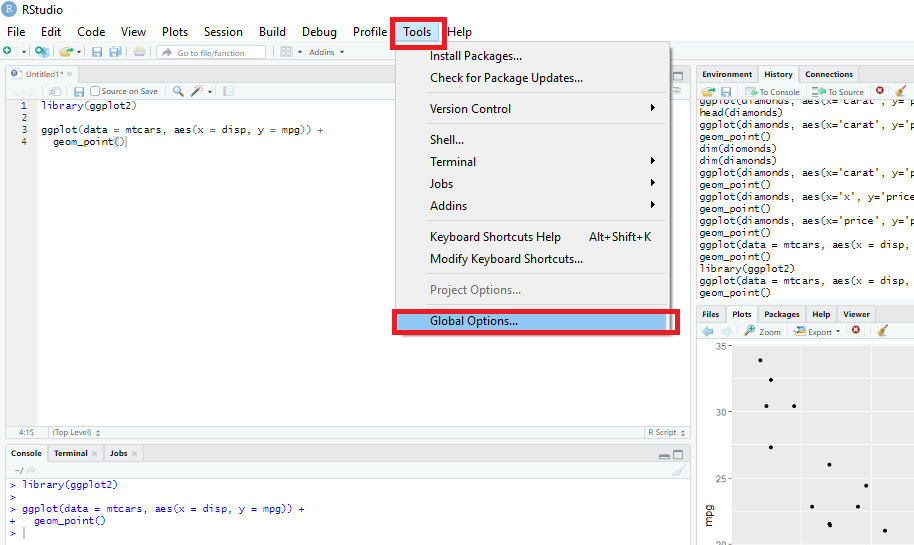
\includegraphics[width=1\linewidth]{figures/rstudio2} \caption{\label{fig:rstudio2} Ferramentas de aparência do RStudio}\label{fig:telarstudio2}
\end{figure}

\begin{figure}
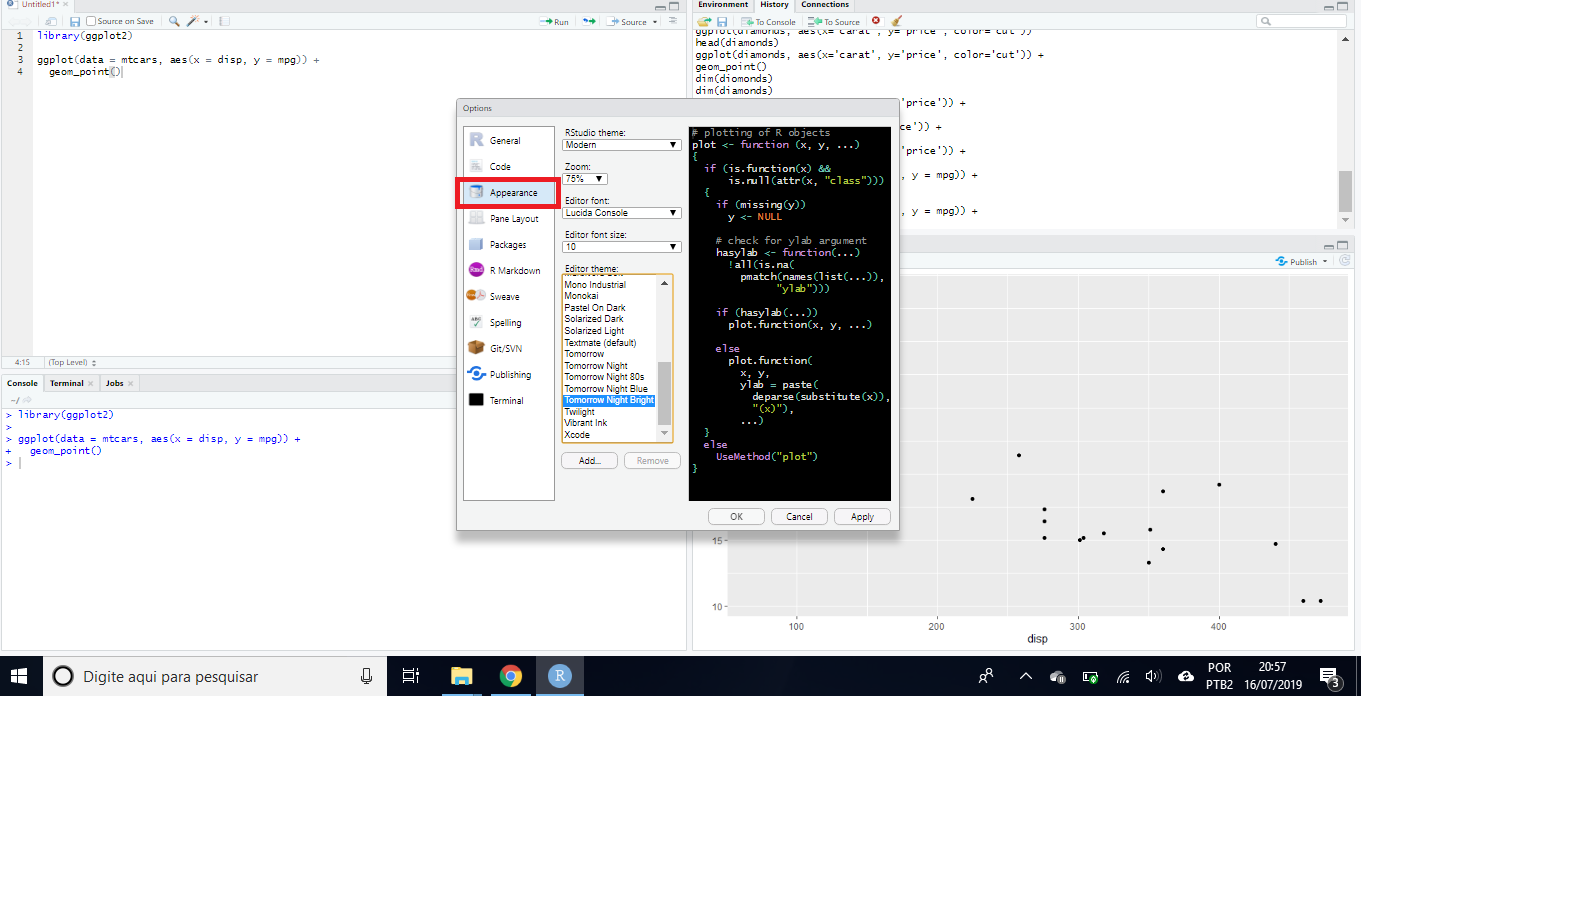
\includegraphics[width=1\linewidth]{figures/rstudio3} \caption{\label{fig:rstudio3} Ferramentas de aparência do RStudio}\label{fig:telarstudio3}
\end{figure}

Ainda no menu Tools --\textgreater{} Global Options --\textgreater{} Pane Layout, o usuário pode organizar a ordem dos quadrantes do RStudio, como apresentado nas Figuras \ref{fig:telarstudio4}, \ref{fig:telarstudio5} e \ref{fig:telarstudio6}. No exemplo, o painel console foi transferido para o lado do painel Script, o que facilita a visualização dos comandos rodados.

\begin{figure}
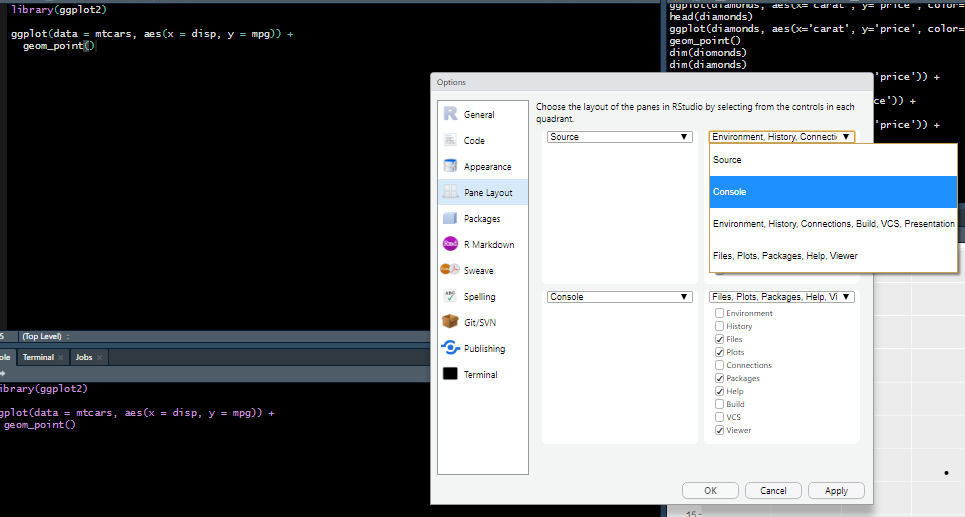
\includegraphics[width=1\linewidth]{figures/rstudio4} \caption{\label{fig:rstudio4} Ferramentas de aparência do RStudio}\label{fig:telarstudio4}
\end{figure}

\begin{figure}
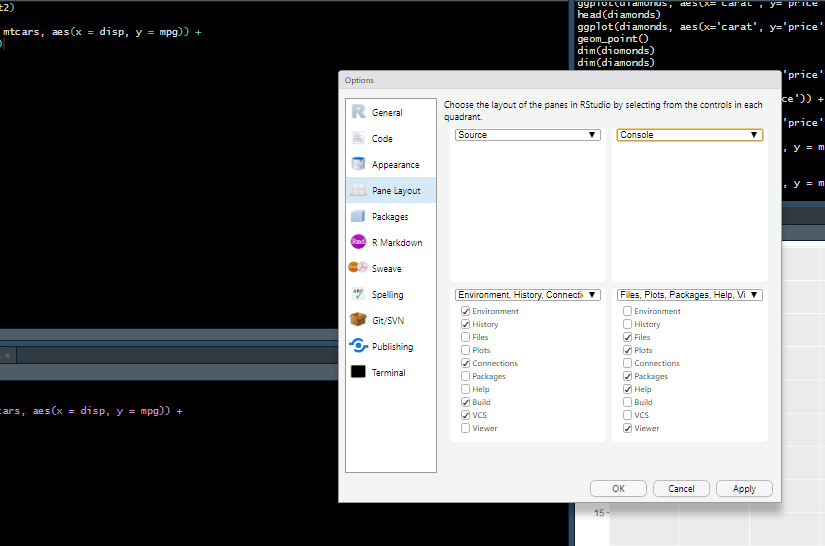
\includegraphics[width=1\linewidth]{figures/rstudio5} \caption{\label{fig:rstudio5} Ferramentas de aparência do RStudio}\label{fig:telarstudio5}
\end{figure}

\begin{figure}
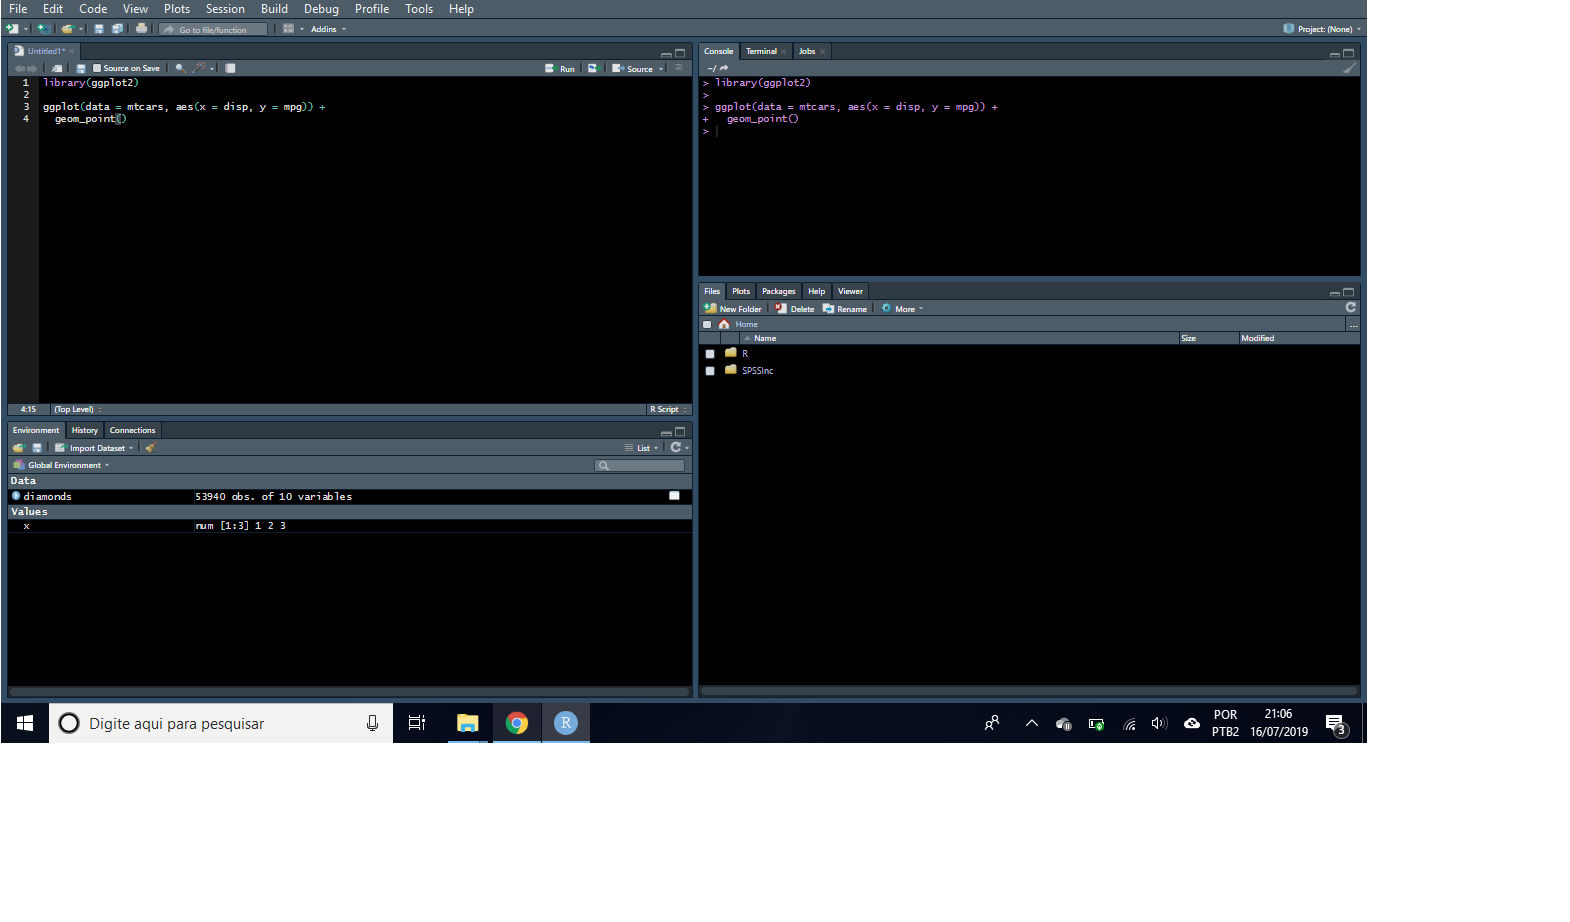
\includegraphics[width=1\linewidth]{figures/rstudio6} \caption{\label{fig:rstudio6} Ferramentas de aparência do RStudio}\label{fig:telarstudio6}
\end{figure}

\hypertarget{projetos}{%
\subsubsection{Projetos}\label{projetos}}

Uma funcionalidade importante é a criação de projetos, permitindo dividir o trabalho em múltiplos ambientes, cada um com o seu diretório, documentos e workspace.

Para criar um projeto, os seguintes passos podem ser seguidos:

\begin{enumerate}
\def\labelenumi{\arabic{enumi})}
\item
  Clique na opção ``File'' do menu, e então em ``New Project''.
\item
  Clique em ``New Directory''.
\item
  Clique em ``New Project''.
\item
  Escreva o nome do diretório (pasta) onde deseja manter seu projeto, ex ``my\_project''.
\item
  Clique no botão ``Create Project''.
\end{enumerate}

Para criar um novo script para escrever os códigos, vá em File -\textgreater{} New File -\textgreater{} R Script

\hypertarget{boas-pruxe1ticas}{%
\subsubsection{Boas práticas}\label{boas-pruxe1ticas}}

Comente bem o seu código: É possível fazer comentários usando o símbolo `\#'. É sempre bom explicar o que uma variável armazena, o que uma função faz, porque alguns parâmetros são passados para uma determinada função, qual é o objetivo de um trecho de código, etc.

Evite linhas de código muito longas: Usar linhas de código mais curtas ajuda na leitura do código.

Escreva um código organizado. Por exemplo, adote um padrão no uso de minúsculas e maiúsculas, uma lógica única na organização de pastas e arquivos, pode ser adotada uma breve descrição (como comentário) indicando o que um determinado script faz.

Carregue todos os pacotes que irá usar sempre no início do arquivo: Quando alguém abrir o seu código será fácil identificar quais são os pacotes que devem ser instalados e quais dependências podem existir.

\hypertarget{primeiros-passos-no-r}{%
\subsection{Primeiros passos no R}\label{primeiros-passos-no-r}}

Posso escrever o código no Script e submeter ao apertar o botão ``Run'' ou com o atalho no teclado Cmd/Ctrl+Enter.

\hypertarget{r-como-calculadora}{%
\subsubsection{R como calculadora}\label{r-como-calculadora}}

\begin{enumerate}
\def\labelenumi{\arabic{enumi})}
\tightlist
\item
  Operadores
\end{enumerate}

\begin{Shaded}
\begin{Highlighting}[]
\CommentTok{#adição}
\DecValTok{10}\OperatorTok{+}\DecValTok{15}
\end{Highlighting}
\end{Shaded}

\begin{verbatim}
## [1] 25
\end{verbatim}

\begin{Shaded}
\begin{Highlighting}[]
\CommentTok{#subtração}
\DecValTok{10-2}
\end{Highlighting}
\end{Shaded}

\begin{verbatim}
## [1] 8
\end{verbatim}

\begin{Shaded}
\begin{Highlighting}[]
\CommentTok{#multiplicação}
\DecValTok{2}\OperatorTok{*}\DecValTok{10}
\end{Highlighting}
\end{Shaded}

\begin{verbatim}
## [1] 20
\end{verbatim}

\begin{Shaded}
\begin{Highlighting}[]
\CommentTok{#divisão}
\DecValTok{30}\OperatorTok{/}\DecValTok{2}
\end{Highlighting}
\end{Shaded}

\begin{verbatim}
## [1] 15
\end{verbatim}

\begin{Shaded}
\begin{Highlighting}[]
\CommentTok{#raiz quadrada}
\KeywordTok{sqrt}\NormalTok{(}\DecValTok{4}\NormalTok{)}
\end{Highlighting}
\end{Shaded}

\begin{verbatim}
## [1] 2
\end{verbatim}

\begin{Shaded}
\begin{Highlighting}[]
\CommentTok{#potência}
\DecValTok{2}\OperatorTok{^}\DecValTok{2}
\end{Highlighting}
\end{Shaded}

\begin{verbatim}
## [1] 4
\end{verbatim}

Se você digitar um comando incompleto, como 10 *, o R mostrará um +. Isso não tem a ver com a soma e apenas que o R está esperando você completar seu comando. Termine seu comando ou aperte Esc para recomeçar.
Vale também ressaltar que se você digitar um comando que o R não reconhece, ele retornará uma mensagem de erro e você pode digitar outro comando normalmente em seguida.

\hypertarget{atribuiuxe7uxe3o}{%
\subsubsection{Atribuição}\label{atribuiuxe7uxe3o}}

Para atribuir a um objeto, o sinal de atribuição é = ou \textless- (preferível).
Exemplos:

\begin{Shaded}
\begin{Highlighting}[]
\NormalTok{x <-}\StringTok{ }\DecValTok{10}\OperatorTok{/}\DecValTok{2}
\NormalTok{x}
\end{Highlighting}
\end{Shaded}

\begin{verbatim}
## [1] 5
\end{verbatim}

\begin{Shaded}
\begin{Highlighting}[]
\NormalTok{X}
\end{Highlighting}
\end{Shaded}

\begin{verbatim}
## Error in eval(expr, envir, enclos): objeto 'X' não encontrado
\end{verbatim}

Por que tivemos um erro acima?

O R é case sensitive, isto é, faz a diferenciação entre as letras minúsculas e maiúsculas. Portanto, x é diferente de X.

\hypertarget{objetos-em-r}{%
\subsubsection{Objetos em R}\label{objetos-em-r}}

Existem cinco classes básicas no R:

\begin{itemize}
\item
  character: ``UAH!''
\item
  numeric: 0.95 (números reais)
\item
  integer: 100515 (inteiros)
\item
  complex: 2 + 5i (números complexos, a + bi)
\item
  logical: TRUE (booleanos, TRUE/FALSE)
\end{itemize}

Vamos atribuir a x a string banana.

\begin{Shaded}
\begin{Highlighting}[]
\NormalTok{x <-}\StringTok{ }\NormalTok{banana }
\end{Highlighting}
\end{Shaded}

\begin{verbatim}
## Error in eval(expr, envir, enclos): objeto 'banana' não encontrado
\end{verbatim}

\begin{Shaded}
\begin{Highlighting}[]
\NormalTok{x <-}\StringTok{ "banana"}
\NormalTok{x}
\end{Highlighting}
\end{Shaded}

\begin{verbatim}
## [1] "banana"
\end{verbatim}

O primeiro caso (x\textless-banana) não deu certo, pois ele entendeu que estamos atribuindo a x outro objeto banana, que não foi declarado. Para atribuir o string banana à x, precisamos colocar entre aspas ou aspas simples. Uma string sem aspas é entendido como um objeto, veja abaixo:

\begin{Shaded}
\begin{Highlighting}[]
\NormalTok{banana <-}\StringTok{ }\DecValTok{30}
\NormalTok{x <-}\StringTok{ }\NormalTok{banana}
\NormalTok{x}
\end{Highlighting}
\end{Shaded}

\begin{verbatim}
## [1] 30
\end{verbatim}

Para saber a classe de um objetivo, use a função class().

\begin{Shaded}
\begin{Highlighting}[]
\NormalTok{y <-}\StringTok{ "ola"}
\KeywordTok{class}\NormalTok{(y)}
\end{Highlighting}
\end{Shaded}

\begin{verbatim}
## [1] "character"
\end{verbatim}

\begin{Shaded}
\begin{Highlighting}[]
\NormalTok{x <-}\StringTok{ }\FloatTok{2.5}
\KeywordTok{class}\NormalTok{(x)}
\end{Highlighting}
\end{Shaded}

\begin{verbatim}
## [1] "numeric"
\end{verbatim}

\hypertarget{apagar-objetos}{%
\subsubsection{Apagar objetos}\label{apagar-objetos}}

E se eu quiser apagar um objeto?

\begin{Shaded}
\begin{Highlighting}[]
\NormalTok{x <-}\StringTok{ }\DecValTok{20}
\NormalTok{x}
\end{Highlighting}
\end{Shaded}

\begin{verbatim}
## [1] 20
\end{verbatim}

\begin{Shaded}
\begin{Highlighting}[]
\KeywordTok{remove}\NormalTok{(x)}
\NormalTok{x}
\end{Highlighting}
\end{Shaded}

\begin{verbatim}
## Error in eval(expr, envir, enclos): objeto 'x' não encontrado
\end{verbatim}

E se eu quiser limpar o console - apaga todos os objetos atribuidos até aqui:

\begin{Shaded}
\begin{Highlighting}[]
\KeywordTok{rm}\NormalTok{(}\DataTypeTok{list=}\KeywordTok{ls}\NormalTok{())}
\end{Highlighting}
\end{Shaded}

\hypertarget{vetor}{%
\subsubsection{Vetor}\label{vetor}}

Como atribuir varios valores a um objeto? Para entrar com vários números (ou nomes, ou qualquer outro grupo de coisas), precisamos usar uma função para dizer ao programa que os valores serão combinados em um único vetor.

\begin{Shaded}
\begin{Highlighting}[]
\NormalTok{x <-}\StringTok{ }\KeywordTok{c}\NormalTok{(}\DecValTok{2}\NormalTok{,}\DecValTok{3}\NormalTok{,}\DecValTok{4}\NormalTok{)}
\NormalTok{x}
\end{Highlighting}
\end{Shaded}

\begin{verbatim}
## [1] 2 3 4
\end{verbatim}

\begin{Shaded}
\begin{Highlighting}[]
\NormalTok{y <-}\StringTok{ }\KeywordTok{seq}\NormalTok{(}\DecValTok{1}\OperatorTok{:}\DecValTok{10}\NormalTok{)}
\NormalTok{y}
\end{Highlighting}
\end{Shaded}

\begin{verbatim}
##  [1]  1  2  3  4  5  6  7  8  9 10
\end{verbatim}

\begin{Shaded}
\begin{Highlighting}[]
\NormalTok{z <-}\StringTok{ }\KeywordTok{rep}\NormalTok{(}\DecValTok{1}\NormalTok{,}\DecValTok{10}\NormalTok{)}
\NormalTok{z}
\end{Highlighting}
\end{Shaded}

\begin{verbatim}
##  [1] 1 1 1 1 1 1 1 1 1 1
\end{verbatim}

\begin{Shaded}
\begin{Highlighting}[]
\NormalTok{a <-}\StringTok{ }\DecValTok{1}\OperatorTok{:}\DecValTok{10}
\NormalTok{a}
\end{Highlighting}
\end{Shaded}

\begin{verbatim}
##  [1]  1  2  3  4  5  6  7  8  9 10
\end{verbatim}

\begin{Shaded}
\begin{Highlighting}[]
\NormalTok{bicho <-}\KeywordTok{c}\NormalTok{(}\StringTok{"macaco"}\NormalTok{,}\StringTok{"pato"}\NormalTok{,}\StringTok{"galinha"}\NormalTok{,}\StringTok{"porco"}\NormalTok{)}
\NormalTok{bicho}
\end{Highlighting}
\end{Shaded}

\begin{verbatim}
## [1] "macaco"  "pato"    "galinha" "porco"
\end{verbatim}

E se quisermos visualizar o conteúdo da posição 2 no vetor bicho?

\begin{Shaded}
\begin{Highlighting}[]
\NormalTok{bicho[}\DecValTok{2}\NormalTok{]}
\end{Highlighting}
\end{Shaded}

\begin{verbatim}
## [1] "pato"
\end{verbatim}

As operações vetoriais podem ser realizadas de maneira bastante intuitiva. Como exemplos:

\begin{Shaded}
\begin{Highlighting}[]
\NormalTok{x <-}\StringTok{ }\KeywordTok{c}\NormalTok{(}\DecValTok{2}\NormalTok{,}\DecValTok{3}\NormalTok{,}\DecValTok{4}\NormalTok{)}
\NormalTok{x}
\end{Highlighting}
\end{Shaded}

\begin{verbatim}
## [1] 2 3 4
\end{verbatim}

\begin{Shaded}
\begin{Highlighting}[]
\NormalTok{ops <-}\StringTok{ }\NormalTok{x}\DecValTok{-1}
\NormalTok{ops}
\end{Highlighting}
\end{Shaded}

\begin{verbatim}
## [1] 1 2 3
\end{verbatim}

\begin{Shaded}
\begin{Highlighting}[]
\NormalTok{k <-}\StringTok{ }\NormalTok{x}\OperatorTok{*}\DecValTok{2}
\NormalTok{k}
\end{Highlighting}
\end{Shaded}

\begin{verbatim}
## [1] 4 6 8
\end{verbatim}

Vamos agora considerar um vetor de pesos em kg e altura em metros de 6 pessoas.

\begin{Shaded}
\begin{Highlighting}[]
\NormalTok{peso <-}\StringTok{ }\KeywordTok{c}\NormalTok{(}\DecValTok{62}\NormalTok{, }\DecValTok{70}\NormalTok{, }\DecValTok{52}\NormalTok{, }\DecValTok{98}\NormalTok{, }\DecValTok{90}\NormalTok{, }\DecValTok{70}\NormalTok{)}
\NormalTok{peso}
\end{Highlighting}
\end{Shaded}

\begin{verbatim}
## [1] 62 70 52 98 90 70
\end{verbatim}

\begin{Shaded}
\begin{Highlighting}[]
\NormalTok{altura <-}\StringTok{ }\KeywordTok{c}\NormalTok{(}\FloatTok{1.70}\NormalTok{, }\FloatTok{1.82}\NormalTok{, }\FloatTok{1.75}\NormalTok{, }\FloatTok{1.94}\NormalTok{, }\FloatTok{1.84}\NormalTok{, }\FloatTok{1.61}\NormalTok{)}
\NormalTok{altura}
\end{Highlighting}
\end{Shaded}

\begin{verbatim}
## [1] 1.70 1.82 1.75 1.94 1.84 1.61
\end{verbatim}

Vale mencionar que o separador de decimais no R é . (ponto)!

Como calcularia o IMC? Lembrando que o IMC é dado pelo peso (em kg) dividido pela altura (em metros) ao quadrado.

\begin{Shaded}
\begin{Highlighting}[]
\NormalTok{imc <-}\StringTok{ }\NormalTok{peso}\OperatorTok{/}\NormalTok{(altura}\OperatorTok{^}\DecValTok{2}\NormalTok{)}
\NormalTok{imc}
\end{Highlighting}
\end{Shaded}

\begin{verbatim}
## [1] 21.45329 21.13271 16.97959 26.03890 26.58318 27.00513
\end{verbatim}

Para saber o tamanho do vetor, use a função length().

\begin{Shaded}
\begin{Highlighting}[]
\KeywordTok{length}\NormalTok{(imc)}
\end{Highlighting}
\end{Shaded}

\begin{verbatim}
## [1] 6
\end{verbatim}

\hypertarget{matrizes}{%
\subsubsection{Matrizes}\label{matrizes}}

Matrizes são vetores numéricos com duas dimensões, que são simplesmente a linha e a coluna às quais o elemento pertence.

\begin{Shaded}
\begin{Highlighting}[]
\NormalTok{x <-}\StringTok{ }\KeywordTok{matrix}\NormalTok{(}\KeywordTok{seq}\NormalTok{(}\DecValTok{1}\OperatorTok{:}\DecValTok{16}\NormalTok{), }\DataTypeTok{nrow=}\DecValTok{4}\NormalTok{,}\DataTypeTok{ncol=}\DecValTok{4}\NormalTok{)}
\NormalTok{x}
\end{Highlighting}
\end{Shaded}

\begin{verbatim}
##      [,1] [,2] [,3] [,4]
## [1,]    1    5    9   13
## [2,]    2    6   10   14
## [3,]    3    7   11   15
## [4,]    4    8   12   16
\end{verbatim}

Note que os números de 1 a 16 foram dispostos na matriz coluna por coluna ou seja, preenchendo de cima para baixo e depois da esquerda para a direita.

Como sei qual elemento está na segunda linha e terceira coluna da matriz x?

\begin{Shaded}
\begin{Highlighting}[]
\NormalTok{x[}\DecValTok{2}\NormalTok{,}\DecValTok{3}\NormalTok{]}
\end{Highlighting}
\end{Shaded}

\begin{verbatim}
## [1] 10
\end{verbatim}

\begin{Shaded}
\begin{Highlighting}[]
\NormalTok{x[}\DecValTok{3}\NormalTok{,  ]   }\CommentTok{# seleciona a 3ª linha}
\end{Highlighting}
\end{Shaded}

\begin{verbatim}
## [1]  3  7 11 15
\end{verbatim}

\begin{Shaded}
\begin{Highlighting}[]
\NormalTok{x[ , }\DecValTok{2}\NormalTok{]   }\CommentTok{# seleciona a 2ª coluna}
\end{Highlighting}
\end{Shaded}

\begin{verbatim}
## [1] 5 6 7 8
\end{verbatim}

\begin{Shaded}
\begin{Highlighting}[]
\NormalTok{x[}\DecValTok{1}\NormalTok{, }\DecValTok{2}\NormalTok{]   }\CommentTok{# seleciona o elemento da primeira linha e segunda coluna}
\end{Highlighting}
\end{Shaded}

\begin{verbatim}
## [1] 5
\end{verbatim}

E se eu quiser substituir a primeira linha por (13,15,19,30)?

\begin{Shaded}
\begin{Highlighting}[]
\NormalTok{x[}\DecValTok{1}\NormalTok{,] <-}\StringTok{ }\KeywordTok{c}\NormalTok{(}\DecValTok{13}\NormalTok{,}\DecValTok{15}\NormalTok{,}\DecValTok{19}\NormalTok{,}\DecValTok{30}\NormalTok{)}

\NormalTok{x}
\end{Highlighting}
\end{Shaded}

\begin{verbatim}
##      [,1] [,2] [,3] [,4]
## [1,]   13   15   19   30
## [2,]    2    6   10   14
## [3,]    3    7   11   15
## [4,]    4    8   12   16
\end{verbatim}

Seja o vetor d

\begin{Shaded}
\begin{Highlighting}[]
\NormalTok{d <-}\StringTok{ }\KeywordTok{c}\NormalTok{(}\DecValTok{128}\NormalTok{,}\DecValTok{124}\NormalTok{,}\DecValTok{213}\NormalTok{,}\DecValTok{234}\NormalTok{)}
\end{Highlighting}
\end{Shaded}

E se quisermos substituir a terceira coluna por d?

\begin{Shaded}
\begin{Highlighting}[]
\NormalTok{x[,}\DecValTok{3}\NormalTok{] <-}\StringTok{ }\NormalTok{d}
\end{Highlighting}
\end{Shaded}

Qual a dimensao da matriz x?

Vimos que para vetor usamos o comando length(). Serve par matriz? Vamos testar:

\begin{Shaded}
\begin{Highlighting}[]
\KeywordTok{length}\NormalTok{(x)}
\end{Highlighting}
\end{Shaded}

\begin{verbatim}
## [1] 16
\end{verbatim}

Note que é retornado o num de colunas vezes o número de linhas (4*4). Mas o que quero saber é o numero de linhas e de colunas. Para isso, o comando é dim().

\begin{Shaded}
\begin{Highlighting}[]
\KeywordTok{dim}\NormalTok{(x)}
\end{Highlighting}
\end{Shaded}

\begin{verbatim}
## [1] 4 4
\end{verbatim}

Para concatenar linhas em uma matriz, podemos usar o comando rbind():

\begin{Shaded}
\begin{Highlighting}[]
\NormalTok{vet <-}\StringTok{ }\KeywordTok{c}\NormalTok{(}\DecValTok{2}\NormalTok{,}\DecValTok{20}\NormalTok{,}\DecValTok{12}\NormalTok{,}\DecValTok{34}\NormalTok{)}
\NormalTok{x2 <-}\StringTok{ }\KeywordTok{rbind}\NormalTok{(x,vet)}
\NormalTok{x2}
\end{Highlighting}
\end{Shaded}

\begin{verbatim}
##     [,1] [,2] [,3] [,4]
##       13   15  128   30
##        2    6  124   14
##        3    7  213   15
##        4    8  234   16
## vet    2   20   12   34
\end{verbatim}

Para concatenar colunas em uma matriz, podemos usar o comando cbind():

\begin{Shaded}
\begin{Highlighting}[]
\NormalTok{v2 <-}\StringTok{ }\KeywordTok{c}\NormalTok{(}\DecValTok{25}\NormalTok{,}\DecValTok{10}\NormalTok{,}\DecValTok{15}\NormalTok{,}\DecValTok{4}\NormalTok{) }
\NormalTok{x3 <-}\StringTok{ }\KeywordTok{cbind}\NormalTok{(x,v2)}
\NormalTok{x3}
\end{Highlighting}
\end{Shaded}

\begin{verbatim}
##                   v2
## [1,] 13 15 128 30 25
## [2,]  2  6 124 14 10
## [3,]  3  7 213 15 15
## [4,]  4  8 234 16  4
\end{verbatim}

\hypertarget{fator}{%
\subsubsection{Fator}\label{fator}}

Fatores podem ser vistos como vetores de inteiros que possuem rótulos (labels). Eles são úteis para representar uma variável categórica (nominal e ordinal).

\begin{Shaded}
\begin{Highlighting}[]
\NormalTok{sexo <-}\StringTok{ }\KeywordTok{c}\NormalTok{(}\StringTok{"M"}\NormalTok{, }\StringTok{"H"}\NormalTok{, }\StringTok{"H"}\NormalTok{, }\StringTok{"H"}\NormalTok{, }\StringTok{"M"}\NormalTok{, }\StringTok{"M"}\NormalTok{, }\StringTok{"H"}\NormalTok{)}
\NormalTok{sex <-}\StringTok{ }\KeywordTok{as.factor}\NormalTok{(sexo)}
\NormalTok{sex}
\end{Highlighting}
\end{Shaded}

\begin{verbatim}
## [1] M H H H M M H
## Levels: H M
\end{verbatim}

\begin{Shaded}
\begin{Highlighting}[]
\KeywordTok{levels}\NormalTok{(sex)}
\end{Highlighting}
\end{Shaded}

\begin{verbatim}
## [1] "H" "M"
\end{verbatim}

\hypertarget{data-frame}{%
\subsubsection{Data frame}\label{data-frame}}

Trata-se de uma ``tabela de dados'' onde as colunas são as variáveis e as linhas são os registros. Essas colunas podem ser de classes diferentes.
Essa é a grande diferença entre data.frame's e matrizes (matriz é só numerica).

Posso criar um data frame no R com os vetores, por exemplo:

\begin{Shaded}
\begin{Highlighting}[]
\NormalTok{ID <-}\StringTok{ }\KeywordTok{seq}\NormalTok{(}\DecValTok{1}\OperatorTok{:}\DecValTok{6}\NormalTok{)}
\NormalTok{pes <-}\StringTok{ }\KeywordTok{c}\NormalTok{(}\DecValTok{62}\NormalTok{, }\DecValTok{70}\NormalTok{, }\DecValTok{52}\NormalTok{, }\DecValTok{98}\NormalTok{, }\DecValTok{90}\NormalTok{, }\DecValTok{70}\NormalTok{)}
\NormalTok{alt <-}\StringTok{ }\KeywordTok{c}\NormalTok{(}\FloatTok{1.70}\NormalTok{, }\FloatTok{1.82}\NormalTok{, }\FloatTok{1.75}\NormalTok{, }\FloatTok{1.94}\NormalTok{, }\FloatTok{1.84}\NormalTok{, }\FloatTok{1.61}\NormalTok{)}
\NormalTok{imc <-}\StringTok{ }\NormalTok{pes}\OperatorTok{/}\NormalTok{(alt}\OperatorTok{^}\DecValTok{2}\NormalTok{)}
\NormalTok{dados <-}\StringTok{ }\KeywordTok{data.frame}\NormalTok{(}\DataTypeTok{ID=}\NormalTok{ID,}\DataTypeTok{peso=}\NormalTok{pes,}\DataTypeTok{altura=}\NormalTok{alt, }\DataTypeTok{imc=}\NormalTok{imc)}
\NormalTok{dados}
\end{Highlighting}
\end{Shaded}

\begin{verbatim}
##   ID peso altura      imc
## 1  1   62   1.70 21.45329
## 2  2   70   1.82 21.13271
## 3  3   52   1.75 16.97959
## 4  4   98   1.94 26.03890
## 5  5   90   1.84 26.58318
## 6  6   70   1.61 27.00513
\end{verbatim}

Posso pensar que o dat frame tem a mesma ideia de matriz. Quero olhar os dados de altura. Sei que altura está na coluna 3.

\begin{Shaded}
\begin{Highlighting}[]
\NormalTok{dados[,}\DecValTok{3}\NormalTok{]}
\end{Highlighting}
\end{Shaded}

\begin{verbatim}
## [1] 1.70 1.82 1.75 1.94 1.84 1.61
\end{verbatim}

Mas existe uma maneira mais facil de selecionar a variavel de interesse:
Por ser um data frame, posso usar \$:

\begin{Shaded}
\begin{Highlighting}[]
\NormalTok{dados}\OperatorTok{$}\NormalTok{altura}
\end{Highlighting}
\end{Shaded}

\begin{verbatim}
## [1] 1.70 1.82 1.75 1.94 1.84 1.61
\end{verbatim}

Putz, esqueci de colocar a varivel de grupo no data frame. Tenho que criar tudo de novo? Não:

\begin{Shaded}
\begin{Highlighting}[]
\NormalTok{gr <-}\StringTok{ }\KeywordTok{c}\NormalTok{(}\KeywordTok{rep}\NormalTok{(}\DecValTok{1}\NormalTok{,}\DecValTok{3}\NormalTok{),}\KeywordTok{rep}\NormalTok{(}\DecValTok{2}\NormalTok{,}\DecValTok{3}\NormalTok{))}
\NormalTok{dados}\OperatorTok{$}\NormalTok{grupo <-}\StringTok{ }\NormalTok{gr}

\NormalTok{dados}
\end{Highlighting}
\end{Shaded}

\begin{verbatim}
##   ID peso altura      imc grupo
## 1  1   62   1.70 21.45329     1
## 2  2   70   1.82 21.13271     1
## 3  3   52   1.75 16.97959     1
## 4  4   98   1.94 26.03890     2
## 5  5   90   1.84 26.58318     2
## 6  6   70   1.61 27.00513     2
\end{verbatim}

Funcoes uteis para data.frame:

\begin{itemize}
\item
  head() - Mostra as primeiras 6 linhas.
\item
  tail() - Mostra as últimas 6 linhas.
\item
  dim() - Número de linhas e de colunas.
\item
  names() - Os nomes das colunas (variáveis).
\item
  str() - Estrutura do data.frame. Mostra, entre outras coisas, as classes de cada coluna.
\end{itemize}

\begin{Shaded}
\begin{Highlighting}[]
\KeywordTok{head}\NormalTok{(dados)}
\end{Highlighting}
\end{Shaded}

\begin{verbatim}
##   ID peso altura      imc grupo
## 1  1   62   1.70 21.45329     1
## 2  2   70   1.82 21.13271     1
## 3  3   52   1.75 16.97959     1
## 4  4   98   1.94 26.03890     2
## 5  5   90   1.84 26.58318     2
## 6  6   70   1.61 27.00513     2
\end{verbatim}

\begin{Shaded}
\begin{Highlighting}[]
\KeywordTok{tail}\NormalTok{(dados)}
\end{Highlighting}
\end{Shaded}

\begin{verbatim}
##   ID peso altura      imc grupo
## 1  1   62   1.70 21.45329     1
## 2  2   70   1.82 21.13271     1
## 3  3   52   1.75 16.97959     1
## 4  4   98   1.94 26.03890     2
## 5  5   90   1.84 26.58318     2
## 6  6   70   1.61 27.00513     2
\end{verbatim}

\begin{Shaded}
\begin{Highlighting}[]
\KeywordTok{dim}\NormalTok{(dados)}
\end{Highlighting}
\end{Shaded}

\begin{verbatim}
## [1] 6 5
\end{verbatim}

\begin{Shaded}
\begin{Highlighting}[]
\KeywordTok{names}\NormalTok{(dados)}
\end{Highlighting}
\end{Shaded}

\begin{verbatim}
## [1] "ID"     "peso"   "altura" "imc"    "grupo"
\end{verbatim}

\begin{Shaded}
\begin{Highlighting}[]
\KeywordTok{str}\NormalTok{(dados)}
\end{Highlighting}
\end{Shaded}

\begin{verbatim}
## 'data.frame':	6 obs. of  5 variables:
##  $ ID    : int  1 2 3 4 5 6
##  $ peso  : num  62 70 52 98 90 70
##  $ altura: num  1.7 1.82 1.75 1.94 1.84 1.61
##  $ imc   : num  21.5 21.1 17 26 26.6 ...
##  $ grupo : num  1 1 1 2 2 2
\end{verbatim}

\hypertarget{operadores-relacionais}{%
\subsubsection{Operadores Relacionais}\label{operadores-relacionais}}

Igual a: ==

Exemplo:

\begin{Shaded}
\begin{Highlighting}[]
\DecValTok{10}\OperatorTok{==}\DecValTok{11}
\end{Highlighting}
\end{Shaded}

\begin{verbatim}
## [1] FALSE
\end{verbatim}

Diferente de: !=

Exemplo:

\begin{Shaded}
\begin{Highlighting}[]
\DecValTok{10}\OperatorTok{!=}\DecValTok{11}
\end{Highlighting}
\end{Shaded}

\begin{verbatim}
## [1] TRUE
\end{verbatim}

\begin{itemize}
\item
  Maior que: \textgreater{}
\item
  Maior ou igual: \textgreater=
\item
  Menor que: \textless{}
\item
  Menor ou igual: \textless=
\end{itemize}

Exemplos:

\begin{Shaded}
\begin{Highlighting}[]
\DecValTok{10}\OperatorTok{>}\DecValTok{5}
\end{Highlighting}
\end{Shaded}

\begin{verbatim}
## [1] TRUE
\end{verbatim}

\begin{Shaded}
\begin{Highlighting}[]
\DecValTok{10}\OperatorTok{>=}\DecValTok{10}
\end{Highlighting}
\end{Shaded}

\begin{verbatim}
## [1] TRUE
\end{verbatim}

\begin{Shaded}
\begin{Highlighting}[]
\DecValTok{4}\OperatorTok{<}\DecValTok{4}
\end{Highlighting}
\end{Shaded}

\begin{verbatim}
## [1] FALSE
\end{verbatim}

\begin{Shaded}
\begin{Highlighting}[]
\DecValTok{4}\OperatorTok{<=}\DecValTok{4}
\end{Highlighting}
\end{Shaded}

\begin{verbatim}
## [1] TRUE
\end{verbatim}

\hypertarget{operadores-luxf3gicos}{%
\subsubsection{Operadores Lógicos}\label{operadores-luxf3gicos}}

\begin{itemize}
\tightlist
\item
  E: \& - será verdadeiro se os dois forem TRUE
\end{itemize}

\begin{Shaded}
\begin{Highlighting}[]
\NormalTok{x <-}\StringTok{ }\DecValTok{15}
\NormalTok{x }\OperatorTok{>}\StringTok{ }\DecValTok{10} \OperatorTok{&}\StringTok{ }\NormalTok{x }\OperatorTok{<}\StringTok{ }\DecValTok{30}
\end{Highlighting}
\end{Shaded}

\begin{verbatim}
## [1] TRUE
\end{verbatim}

\begin{Shaded}
\begin{Highlighting}[]
\NormalTok{x }\OperatorTok{<}\StringTok{ }\DecValTok{10} \OperatorTok{&}\StringTok{ }\NormalTok{x }\OperatorTok{<}\StringTok{ }\DecValTok{30}
\end{Highlighting}
\end{Shaded}

\begin{verbatim}
## [1] FALSE
\end{verbatim}

\begin{itemize}
\tightlist
\item
  OU: \textbar{} - será verdadeiro se um dos dois forem TRUE
\end{itemize}

\begin{Shaded}
\begin{Highlighting}[]
\NormalTok{x <-}\StringTok{ }\DecValTok{15}
\NormalTok{x }\OperatorTok{>}\StringTok{ }\DecValTok{10} \OperatorTok{|}\StringTok{ }\NormalTok{x }\OperatorTok{<}\StringTok{ }\DecValTok{30}
\end{Highlighting}
\end{Shaded}

\begin{verbatim}
## [1] TRUE
\end{verbatim}

\begin{Shaded}
\begin{Highlighting}[]
\NormalTok{x }\OperatorTok{<}\StringTok{ }\DecValTok{10} \OperatorTok{|}\StringTok{ }\NormalTok{x }\OperatorTok{<}\StringTok{ }\DecValTok{30}
\end{Highlighting}
\end{Shaded}

\begin{verbatim}
## [1] TRUE
\end{verbatim}

\begin{itemize}
\tightlist
\item
  Negação: !
\end{itemize}

\begin{Shaded}
\begin{Highlighting}[]
\NormalTok{x <-}\StringTok{ }\DecValTok{15}
\OperatorTok{!}\NormalTok{x}\OperatorTok{<}\DecValTok{30}
\end{Highlighting}
\end{Shaded}

\begin{verbatim}
## [1] FALSE
\end{verbatim}

\hypertarget{if-e-else}{%
\subsubsection{If e else}\label{if-e-else}}

\begin{Shaded}
\begin{Highlighting}[]
\NormalTok{a <-}\StringTok{ }\DecValTok{224}
\NormalTok{b <-}\StringTok{ }\DecValTok{225}
\ControlFlowTok{if}\NormalTok{ (a}\OperatorTok{==}\NormalTok{b) \{ v=}\DecValTok{10}
\NormalTok{\} }\ControlFlowTok{else}\NormalTok{ \{v=}\DecValTok{15}\NormalTok{\}}
\NormalTok{v}
\end{Highlighting}
\end{Shaded}

\begin{verbatim}
## [1] 15
\end{verbatim}

\begin{Shaded}
\begin{Highlighting}[]
\NormalTok{a <-}\StringTok{ }\DecValTok{224}
\NormalTok{b <-}\StringTok{ }\DecValTok{225}
\ControlFlowTok{if}\NormalTok{ (a}\OperatorTok{==}\NormalTok{b) \{ v=}\DecValTok{10}
\NormalTok{\} }\ControlFlowTok{else} \ControlFlowTok{if}\NormalTok{ (a }\OperatorTok{>}\StringTok{ }\NormalTok{b) \{v=}\DecValTok{15}
\NormalTok{\} }\ControlFlowTok{else}\NormalTok{ \{v=}\DecValTok{25}\NormalTok{\}}
\NormalTok{v}
\end{Highlighting}
\end{Shaded}

\begin{verbatim}
## [1] 25
\end{verbatim}

Note que a condição de igualdade é representada por dois iguais ==. Como dito anteriormente, apenas um igual = é símbolo de atribuição (mas preferível \textless-).

\hypertarget{for}{%
\subsubsection{For}\label{for}}

Seja o vetor m dado por:

\begin{Shaded}
\begin{Highlighting}[]
\NormalTok{m <-}\StringTok{ }\KeywordTok{c}\NormalTok{(}\DecValTok{1}\NormalTok{,}\DecValTok{20}\NormalTok{,}\DecValTok{50}\NormalTok{,}\DecValTok{60}\NormalTok{,}\DecValTok{100}\NormalTok{)}
\end{Highlighting}
\end{Shaded}

Quero criar um novo vetor, p digamos, que seja formado por cada elemento
de m dividido por sua posição.

\begin{Shaded}
\begin{Highlighting}[]
\NormalTok{p <-}\StringTok{ }\OtherTok{NULL}
\ControlFlowTok{for}\NormalTok{ (i }\ControlFlowTok{in} \DecValTok{1}\OperatorTok{:}\StringTok{ }\KeywordTok{length}\NormalTok{(m))\{}
\NormalTok{  p[i] <-}\StringTok{ }\NormalTok{m[i]}\OperatorTok{/}\NormalTok{i}
\NormalTok{\}}
\NormalTok{p}
\end{Highlighting}
\end{Shaded}

\begin{verbatim}
## [1]  1.00000 10.00000 16.66667 15.00000 20.00000
\end{verbatim}

Note que primeiro definimos o objeto p.~

\hypertarget{funuxe7uxf5es}{%
\subsubsection{Funções}\label{funuxe7uxf5es}}

Vamos criar uma função que soma seus dois argumentos.

\begin{Shaded}
\begin{Highlighting}[]
\NormalTok{f.soma <-}\StringTok{ }\ControlFlowTok{function}\NormalTok{(x,y) \{}
\NormalTok{  out <-}\StringTok{ }\NormalTok{x}\OperatorTok{+}\NormalTok{y}
  \KeywordTok{return}\NormalTok{(out)}
\NormalTok{\}}
\end{Highlighting}
\end{Shaded}

A função acima tem:
* o nome: f.soma;

\begin{itemize}
\item
  os argumentos: x e y;
\item
  o corpo out \textless- x+y e
\item
  o que retorna return(out).
\end{itemize}

Vamos agora chamar a função:

\begin{Shaded}
\begin{Highlighting}[]
\KeywordTok{f.soma}\NormalTok{(}\DataTypeTok{x=}\DecValTok{10}\NormalTok{,}\DataTypeTok{y=}\DecValTok{20}\NormalTok{)}
\end{Highlighting}
\end{Shaded}

\begin{verbatim}
## [1] 30
\end{verbatim}

\begin{Shaded}
\begin{Highlighting}[]
\KeywordTok{f.soma}\NormalTok{(}\DecValTok{10}\NormalTok{,}\DecValTok{20}\NormalTok{)}
\end{Highlighting}
\end{Shaded}

\begin{verbatim}
## [1] 30
\end{verbatim}

\hypertarget{dados-faltantes-infinitos-e-indefiniuxe7uxf5es-matemuxe1ticas}{%
\subsubsection{Dados faltantes, infinitos e indefinições matemáticas}\label{dados-faltantes-infinitos-e-indefiniuxe7uxf5es-matemuxe1ticas}}

\begin{itemize}
\item
  NA (Not Available): dado faltante/indisponível.
\item
  NaN (Not a Number): indefinições matemáticas. Como 0/0 e log(-1).
\item
  Inf (Infinito): número muito grande ou o limite matemático. Aceita sinal negativo -Inf.
\end{itemize}

\hypertarget{como-obter-ajuda-no-r}{%
\section{Como obter ajuda no R}\label{como-obter-ajuda-no-r}}

Listamos aqui 3 maneiras para buscar ajuda no R:

\begin{itemize}
\tightlist
\item
  Help/documentação do R (comandos help(nome\_da\_funcao) ou ?nome\_da\_funcao). Como exemplo,
\end{itemize}

\begin{Shaded}
\begin{Highlighting}[]
\KeywordTok{help}\NormalTok{(mean) }\CommentTok{#ou}
\NormalTok{?mean}
\end{Highlighting}
\end{Shaded}

\begin{itemize}
\tightlist
\item
  Google.
  Na Figura \ref{fig:help} está o exemplo de busca de ajuda no Google. Repare no `r' no início da busca, isso pode ajudar.

  \begin{figure}
  
\includegraphics[width=1\linewidth]{figures/help_R} \caption{\label{fig:help}Pesquisa no Google}\label{fig:help}
  \end{figure}
\item
  Comunidade.
\end{itemize}

O \href{https://stackoverflow.com/}{Stack Overflow} e o \href{https://pt.stackoverflow.com/}{Stack Overflow em Português} são sites de Pergunta e Resposta amplamente utilizados por todas as linguagens de programação, e o R é uma delas.

\hypertarget{pacotes}{%
\section{Pacotes}\label{pacotes}}

Como dito quando falamos ``Sobre o R'', o R apresenta funções na sua base e também em forma de pacotes (conjunto de funções bem documentado), que precisam ser instalados (uma vez no seu computador) e carregados na sessão de utilização do R (carregado em toda sessão aberta).

Dificilmente você vai fazer uma análise apenas com as funções básicas do R e dificilmente não vai existir um pacote com as funções que você precisa. Por esse motivo, falamos a seguir em como instalar e carregar pacotes.

\hypertarget{instalauxe7uxe3o}{%
\subsection{Instalação}\label{instalauxe7uxe3o}}

\begin{itemize}
\tightlist
\item
  \textbf{Via CRAN:}
\end{itemize}

\begin{Shaded}
\begin{Highlighting}[]
\KeywordTok{install.packages}\NormalTok{(}\StringTok{"nome-do-pacote"}\NormalTok{)}
\end{Highlighting}
\end{Shaded}

Exemplo: Instalação do pacote \texttt{dplyr}.

\begin{Shaded}
\begin{Highlighting}[]
\KeywordTok{install.packages}\NormalTok{(}\StringTok{"dplyr"}\NormalTok{)}
\end{Highlighting}
\end{Shaded}

Note que o nome do pacote está entre aspas.

\begin{itemize}
\tightlist
\item
  \textbf{Via Github:}
  Para instalar via Github, precisa primeiramente instalar o pacote \texttt{devtools}.
\end{itemize}

\begin{Shaded}
\begin{Highlighting}[]
\NormalTok{devtools}\OperatorTok{::}\KeywordTok{install_github}\NormalTok{(}\StringTok{"nome-do-repo/nome-do-pacote"}\NormalTok{)}
\end{Highlighting}
\end{Shaded}

Exemplo:

\begin{Shaded}
\begin{Highlighting}[]
\NormalTok{devtools}\OperatorTok{::}\KeywordTok{install_github}\NormalTok{(}\StringTok{"tidyverse/dplyr"}\NormalTok{)}
\end{Highlighting}
\end{Shaded}

\hypertarget{carregar-pacotes}{%
\subsection{Carregar pacotes:}\label{carregar-pacotes}}

Uma vez um pacote de interesse instalado em sua máquina, para carregar um pacote na sessão atual do R é só rodar a seguinte linha de comando:

\begin{Shaded}
\begin{Highlighting}[]
\KeywordTok{library}\NormalTok{(nome}\OperatorTok{-}\NormalTok{do}\OperatorTok{-}\NormalTok{pacote)}
\end{Highlighting}
\end{Shaded}

Veja que para carregar o pacote, não usa aspas.

Como exemplo, o carregamento do pacote \texttt{dplyr}:

\begin{Shaded}
\begin{Highlighting}[]
\KeywordTok{library}\NormalTok{(dplyr)}
\end{Highlighting}
\end{Shaded}

Só é necessário instalar o pacote uma vez, mas precisa carregá-lo toda vez que começar uma nova sessão.

Uma vez que o pacote carregado ao rodar a função \texttt{library()}, todas as funções desse pacote podem ser usadas sem problemas.

Caso você não queira carregar o pacote e apenas usar uma função específica do pacote, você pode usar \texttt{nome-do-pacote::nome-da-funcao}. Por exemplo:

\begin{Shaded}
\begin{Highlighting}[]
\NormalTok{dplyr}\OperatorTok{::}\KeywordTok{distinct}\NormalTok{(...)}
\end{Highlighting}
\end{Shaded}

Se você tivesse carregado o pacote \texttt{dplyr} anteriormente (pela função \texttt{library()}), não seria necessário colocar \texttt{dplyr::} antes da função \texttt{distinct} do pacote.

\hypertarget{materiais-complementares}{%
\section{Materiais complementares}\label{materiais-complementares}}

\begin{itemize}
\item
  Critical Thinking in Clinical Research. Felipe Fregni \& Ben M. W. Illigens. 2018.
\item
  Sites:

  \begin{itemize}
  \item
    \url{https://www.bmj.com/about-bmj/resources-readers/publications/statistics-square-one/1-data-display-and-summary}
  \item
    \url{http://www.sthda.com/english/wiki/statistical-tests-and-assumptions}
  \end{itemize}
\item
  CHAPTER 3: Selecting the Study Population. In: Critical Thinking in Clinical Research by Felipe Fregni and Ben Illigens. Oxford University Press 2018.
\item
  Fandino W. Formulating a good research question: Pearls and pitfalls. Indian J Anaesth. 2019;63(8):611--616. \url{doi:10.4103/ija.IJA_198_19}
\item
  Riva JJ, Malik KM, Burnie SJ, Endicott AR, Busse JW. What is your research question? An introduction to the PICOT format for clinicians. J Can Chiropr Assoc. 2012;56(3):167--171.
\item
  External validity, generalizability, and knowledge utilization. Ferguson L1. J Nurs Scholarsh. 2004;36(1):16-22.
\item
  Peter M Rothwell; Commentary: External validity of results of randomized trials: disentangling a complex concept, International Journal of Epidemiology, Volume 39, Issue 1, 1 February 2010, Pages 94--96, \url{https://doi.org/10.1093/ije/dyp305}
\end{itemize}

\hypertarget{conceitos-iniciais}{%
\chapter{Conceitos iniciais}\label{conceitos-iniciais}}

\hypertarget{populauxe7uxe3o}{%
\section{População}\label{populauxe7uxe3o}}

A população é o conjunto de todos os elementos sob investigação, é sobre quem é a pergunta. São alguns exemplos:

\begin{enumerate}
\def\labelenumi{\arabic{enumi}.}
\tightlist
\item
  Deseja-se avaliar se a discordância de peso de fetos gemelares aumenta o risco de óbito fetal.
\end{enumerate}

\textbf{População}: Fetos gemelares.

\begin{enumerate}
\def\labelenumi{\arabic{enumi}.}
\setcounter{enumi}{1}
\tightlist
\item
  Deseja-se saber se um novo tratamento para hipertensão grave é ou não efetivo.
\end{enumerate}

\textbf{População}: Todas as pessoas que sofrem de hipertensão grave.

No estudo sobre o uso de progesterona em gestaçoes gemelares, uma pessoa bem intencionada, mas sem conhecimento de Estatística, poderia pensar: ``como gestação gemelar é de alto risco para prematuridade, assim como gestação com colo curto, em que neste último já é protocolo o uso de progesterona, podemos também usar progesterona em gestações gemelares sem a necessidade de estudo para essa população''. No entanto, esse raciocínio não está correto, pois nos estudos de colo curto só consideram gestações únicas, ou seja, não é estudada a população de gestações gemelares.

Essa discussão é importante, pois a extrapolação de resultado de uma população para outra não tem embasamento Estatístico e qualquer tipo de extrapolação dessa natureza deveria ser evitada.

\hypertarget{amostra}{%
\section{Amostra}\label{amostra}}

Muitas vezes não é possível acessar toda a população para estudarmos as características de interesse. Essa impossibilidade pode ser devido à razões econômicas, geográficas e/ou éticas.

Devido às dificuldades para se observar todos os elementos da população, alguns deles são considerados para o estudo. Este subconjunto representativo da população é denominado de \textbf{amostra}.

\begin{figure}
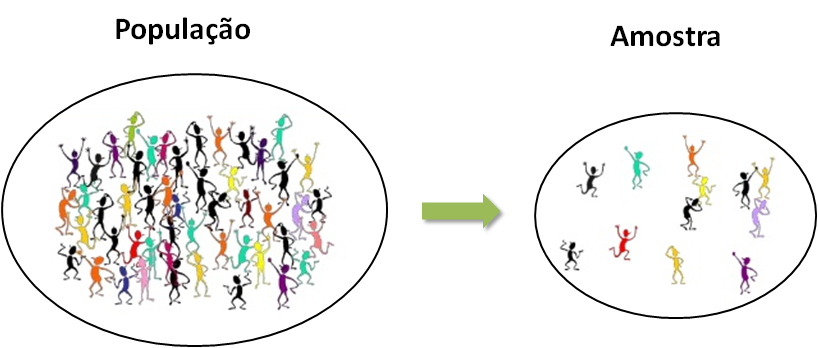
\includegraphics[width=1\linewidth]{figures/esquma_pop_amos} \caption{\label{fig:popamos}Esquema de população e amostra}\label{fig:popAmostra}
\end{figure}

Assim, a motivação de obter uma amostra se deve pela inviabilidade ou até mesmo impossibilidade de se observar toda a população. Como vantagens da amostra, podemos citar: redução de custos, redução de tempo de coleta e reproduz satisfatoriamente a realidade, se a amostra for representativa. A desvantagem se deve pelo motivo desta poder carregar vícios quando feita sem os devidos cuidados.

A técnica considerada para selecionar amostra representativa da população de interesse é a \textbf{amostragem}. A escolha da técnica de amostragem depende de muitas questões e decisões específicas de cada projeto.

Pela experiência em pesquisas na área médica, a definição da técnica de amostragem não é suficiente quando é planejada a coleta da amostra. O que precisa ser definido é o plano amostral.

\begin{quote}
\textbf{Plano amostral:}
Estratégias e especificações metodológicas e estatísticas com o intuito de avaliar a questão científica de maneira adequada.
\end{quote}

No plano amostral, algumas questões precisam ser pensadas:

\begin{itemize}
\item
  Está claramente definida a população de interesse?
\item
  O desenho do estudo é adequado?
\item
  Como será a amostragem?
\item
  O tamanho da amostra é suficiente?
\item
  Estão bem definidas as limitações do estudo?
\item
  O estudo é viável frente a custo, tempo e disponibilidade das unidades?
\item
  Existem variáveis confundidoras?
\item
  Devo pensar em uma análise entre observadores?
\end{itemize}

\hypertarget{variaveis}{%
\section{Variáveis}\label{variaveis}}

Definimos aqui uma variável como sendo uma característica de interesse associada a uma população. Uma variável pode ser classificada em dois tipos:

\begin{itemize}
\item
  \textbf{Qualitativas}: apresentam como possíveis realizações uma qualidade (ou atributo) do indivíduo pesquisado. Exemplos: sexo, grau de instrução, estado civil, classe social, presença de diabetes (sim ou não), etc.
\item
  \textbf{Quantitativas}: apresentam como possíveis realizações números resultantes de uma contagem ou de uma mensuração. Exemplos: Número de filhos, salário, temperatura, pressão arterial, concentração de alguma substância, etc.
\end{itemize}

Ainda, uma \textbf{variável qualitativa} pode ser dividida em \textbf{ordinal} ou \textbf{nominal}, em que:

\begin{itemize}
\item
  \textbf{ordinal}: Existe uma ordem nos seus resultados.
  Exemplo: grau de instrução, estadiamento de uma doença, etc.
\item
  \textbf{nominal}: Não existe nenhuma ordenação nas possíveis realizações.
  Exemplo: Sexo, estado civil, presença de diabetes, etc.
\end{itemize}

Já uma \textbf{variável quantitativa} pode ser dividida em \textbf{discreta} ou \textbf{contínua}, em que:

\begin{itemize}
\tightlist
\item
  \textbf{discreta}: Possíveis valores formam um conjunto finito ou enumerável de pontos e que resultam, frequentemente, de uma contagem. Exemplo:
  número de filhos (0,1,2,\ldots), quantidade de acidentes em um mês (0, 1, 2, \ldots), número de carros que passam no pedágio de Vitória para Vila Velha em 1 hora, etc.
\item
  \textbf{contínua}: Características mensuráveis que assumem valores em um intervalo de números reais. Exemplo: salário, temperatura, pressão arterial, etc.
\end{itemize}

Podemos resumir os tipos de variáveis como o esquema na Figura \ref{fig:tiposVars}.

\begin{figure}
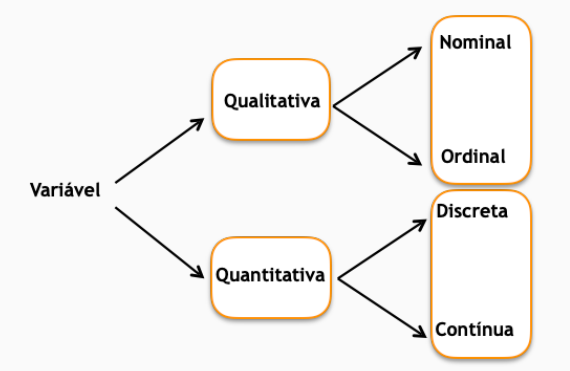
\includegraphics[width=1\linewidth]{figures/tipos_variaveis} \caption{Esquema dos tipos de variáveis}\label{fig:tiposVars}
\end{figure}

A identificação do tipo de variável é importante para a tabulação de dados de maneira correta e também para realizar a análise dos dados de maneira adequada. A seguir falamos sobre a tabulação de dados.

\hypertarget{tabulauxe7uxe3o-de-dados}{%
\section{Tabulação de dados}\label{tabulauxe7uxe3o-de-dados}}

Bases de dados são estruturas organizadas com o objetivo de permitir sua análise estatística. Em geral, cada linha
da planilha corresponde a uma unidade de investigação e cada coluna corresponde a uma variável.

O início dos trabalhos da tabulação dos dados deve ser feito antes da coleta de dados. O planejamento da planilha contribui tanto para o entendimento do processo de coleta de dados quanto para a especificação das variáveis a serem avaliadas. Uma das primeiras medidas é a elaboração de um dicionário com a especificação das variáveis.

Para mais detalhes sobre tabulação de dados, acesse \url{https://daslab-ufes.github.io/materiais/} e clique em ``Tabulacao de Dados''.

\hypertarget{importauxe7uxe3o-de-dados-no-r}{%
\section{Importação de dados no R}\label{importauxe7uxe3o-de-dados-no-r}}

\hypertarget{extensuxe3o-.txt-ou-.csv}{%
\subsection{Extensão .txt ou .csv}\label{extensuxe3o-.txt-ou-.csv}}

Para importar dados para o R, com extensão .txt ou .csv, uma sugestão é utilizar o pacote readr. Como exemplo, consideramos um arquivo chamado dados1.

\begin{Shaded}
\begin{Highlighting}[]
\KeywordTok{library}\NormalTok{(readr)}
\NormalTok{dados_csv <-}\StringTok{ }\KeywordTok{read_csv}\NormalTok{(}\DataTypeTok{file =} \StringTok{"dados1.csv"}\NormalTok{)}
\NormalTok{dados_txt <-}\StringTok{ }\KeywordTok{read_delim}\NormalTok{(}\DataTypeTok{file =} \StringTok{"caminho-para-o-arquivo/dados1.txt"}\NormalTok{, }\DataTypeTok{delim =} \StringTok{" "}\NormalTok{)}
\end{Highlighting}
\end{Shaded}

O argumento file= representa o caminho onde o arquivo está alocado. Se o arquivo estiver no diretório de trabalho, não precisa especificar o caminho até o arquivo. O argumento delim= indica qual caracter separa cada coluna no arquivo de texto.

Outra opção para leitura de arquivo .txt é usar a função read.table que já está salva na base, ou seja, não é necessário instalar pacote.

\begin{Shaded}
\begin{Highlighting}[]
\NormalTok{dados_txt2 <-}\StringTok{ }\KeywordTok{read.table}\NormalTok{(}\DataTypeTok{file=}\StringTok{"dados1.txt"}\NormalTok{,}\DataTypeTok{header=}\NormalTok{T)}
\end{Highlighting}
\end{Shaded}

O argumento header indica se a primeira linha do arquivo consta o nome das variáveis. Se for T (TRUE), a primeira linha é indicada como nome das variáveis. O default é header=F.

Vale ressaltar que para cada função read\_, existe uma respectiva função write\_ para salvar o arquivo no formato de interesse. Como exemplo, queremos salvar a base de dados cars.

\begin{Shaded}
\begin{Highlighting}[]
\KeywordTok{write_csv}\NormalTok{(}\DataTypeTok{x =}\NormalTok{ mtcars, }\DataTypeTok{path =} \StringTok{"cars.csv"}\NormalTok{)}
\KeywordTok{write_delim}\NormalTok{(}\DataTypeTok{x =}\NormalTok{ mtcars, }\DataTypeTok{delim =} \StringTok{" "}\NormalTok{, }\DataTypeTok{path =} \StringTok{"cars.txt"}\NormalTok{)}\ErrorTok{)}
\end{Highlighting}
\end{Shaded}

\hypertarget{arquivos-em-excel}{%
\subsection{Arquivos em Excel}\label{arquivos-em-excel}}

O pacote readxl pode ser utilizado para leiturade arquivos do Excel, como .xls e xlsx.

\begin{Shaded}
\begin{Highlighting}[]
\KeywordTok{library}\NormalTok{(readxl)}
\NormalTok{dados_excel <-}\StringTok{ }\KeywordTok{read_xls}\NormalTok{(}\DataTypeTok{path =} \StringTok{"dados1.xls"}\NormalTok{) }\CommentTok{#Leitura do arquivo .xls}
\NormalTok{dados_excelx <-}\StringTok{ }\KeywordTok{read_xlsx}\NormalTok{(}\DataTypeTok{path =} \StringTok{"dados1.xlsx"}\NormalTok{) }\CommentTok{#Leitura do arquivo .xlsx}
\end{Highlighting}
\end{Shaded}

Uma maneira mais simples é a utilização da função read\_excel(), pois ela auto detecta a extensão do arquivo.

\begin{Shaded}
\begin{Highlighting}[]
\KeywordTok{library}\NormalTok{(readxl)}
\NormalTok{dados_excel1 <-}\StringTok{ }\KeywordTok{read_excel}\NormalTok{(}\DataTypeTok{path =} \StringTok{"dados1.xls"}\NormalTok{)}
\NormalTok{dados_excelx1 <-}\StringTok{ }\KeywordTok{read_excel}\NormalTok{(}\DataTypeTok{path =} \StringTok{"dados1.xlsx"}\NormalTok{)}
\end{Highlighting}
\end{Shaded}

\hypertarget{arquivos-de-outros-softwares}{%
\subsection{Arquivos de outros softwares}\label{arquivos-de-outros-softwares}}

Para ler dados salvos em extensão de outros softwares: SPSS, STATA e SAS, podem ser utilizadas as funções do pacote haven.

\begin{Shaded}
\begin{Highlighting}[]
\KeywordTok{library}\NormalTok{(haven)}
\NormalTok{dados_stata <-}\StringTok{ }\KeywordTok{read_stata}\NormalTok{(}\StringTok{"dados1.dta"}\NormalTok{)}
\NormalTok{dados_spss <-}\StringTok{ }\KeywordTok{read_spss}\NormalTok{(}\StringTok{"dados1.sav"}\NormalTok{)}
\NormalTok{dados_sas <-}\StringTok{ }\KeywordTok{read_sas}\NormalTok{(}\StringTok{"dados1.sas7bdat"}\NormalTok{)  }
\end{Highlighting}
\end{Shaded}

Outra opção de pacote para importação de dados de outros softwares é o foreign. Além do SAS, STAT e SPSS, ele também lê dados do Octave, Minitab e Epi Info.

\hypertarget{consistencia}{%
\section{Análise de consistência e tratamento dos dados}\label{consistencia}}

O tratamento dos dados toma muitas vezes a maior parte do tempo de uma análise estatística.

A análise de consistência consiste em realizar uma primeira análise dos dados com o intuito de encontrar inconsistências. São exemplos de inconsistências:

\begin{itemize}
\tightlist
\item
  boas práticas para nome das variáveis.
\item
  como erros de digitação;
\item
  indivíduos imputados mais de uma vez na planilha de dados de maneira errada;
\item
  identificar casos missings e avaliar se a observação está ausente de maneira correta ou não;
\item
  identificar as categorias de variáveis qualitativas.
\end{itemize}

Para exemplificar o que for discutido, consideramos os dados fictícios de \(n=104\) gestações gemelares, apresentado no Capítulo 2. O dicionário contém a explicação das variáveis, a identificação dos valores ausentes de cada variável e o rótulo das categorias de variáveis qualitativas. Uma boa prática na tabulação dos dados é manter o dicionário junto com a base de dados. Se a tabulação for realizada no Excel, por exemplo, manter o dicionário em uma outra aba.

\hypertarget{importauxe7uxe3o-dos-dados}{%
\subsection{Importação dos dados}\label{importauxe7uxe3o-dos-dados}}

\begin{Shaded}
\begin{Highlighting}[]
\KeywordTok{library}\NormalTok{(readxl)}
\NormalTok{dados <-}\StringTok{ }\KeywordTok{read_excel}\NormalTok{(}\DataTypeTok{path =} \StringTok{"dataset/dados_gemelares.xlsx"}\NormalTok{)}
\NormalTok{dados}
\end{Highlighting}
\end{Shaded}

\begin{verbatim}
## # A tibble: 108 x 21
##       ID Grupo CORION `Data aval`         `Data nascimento`   `COR BRANCO`
##    <dbl> <dbl> <chr>  <dttm>              <dttm>                     <dbl>
##  1     1     2 Di     2017-04-23 00:00:00 1988-04-30 00:00:00            1
##  2     2     1 Mono   2016-03-21 00:00:00 1982-03-30 00:00:00            1
##  3     2     1 Mono   2016-03-21 00:00:00 1982-03-30 00:00:00            1
##  4     3     1 Di     2016-02-17 00:00:00 1991-02-23 00:00:00            2
##  5     5     2 Di     2017-04-23 00:00:00 1988-04-30 00:00:00            2
##  6     6     1 Di     2016-03-21 00:00:00 1989-03-28 00:00:00            2
##  7     7     2 Di     2016-02-17 00:00:00 1985-02-24 00:00:00            2
##  8     8     1 Di     2017-12-14 00:00:00 1988-12-21 00:00:00            1
##  9     9     1 Di     2017-04-23 00:00:00 1980-05-02 00:00:00            3
## 10    10     2 Di     2016-03-21 00:00:00 1984-03-29 00:00:00            1
## # ... with 98 more rows, and 15 more variables: `Peso Pré` <dbl>, ALT <dbl>,
## #   Gesta <dbl>, Para <dbl>, Aborto <dbl>, IND_AP <dbl>, Tabagismo <dbl>,
## #   Alcool <dbl>, Drogas <dbl>, IG_Aval <dbl>, MedidaColo <dbl>,
## #   Num_contra_CTG <dbl>, `IGP semana` <dbl>, `IGP dia` <dbl>, oi <lgl>
\end{verbatim}

\textbf{Exercício}: Na base em excel, substitua o espaço em branco (dados faltantes) por NA e rode o seguinte comando:

\begin{Shaded}
\begin{Highlighting}[]
\NormalTok{dados <-}\StringTok{ }\KeywordTok{read_excel}\NormalTok{(}\DataTypeTok{path =} \StringTok{"dataset/dados_gemelares.xlsx"}\NormalTok{,}\DataTypeTok{na=}\StringTok{"NA"}\NormalTok{)}
\end{Highlighting}
\end{Shaded}

O default do missing é o espaço em branco. Acesse o help em ?read\_excel e veja na = "".

\hypertarget{arrumauxe7uxe3o-da-base-de-dados}{%
\subsection{Arrumação da base de dados}\label{arrumauxe7uxe3o-da-base-de-dados}}

Inicialmente, vamos verificar os nomes das variáveis na base de dados por meio da função \texttt{names}. Note que os nomes tem letras maiúsculas, espaços e acento. Utilizar os dados com essas características não impossibilita as futuras análises, mas pode atrapalhar quando precisamos selecionar algumas dessas variáveis.

\begin{Shaded}
\begin{Highlighting}[]
\KeywordTok{names}\NormalTok{(dados)}
\end{Highlighting}
\end{Shaded}

\begin{verbatim}
##  [1] "ID"              "Grupo"           "CORION"          "Data aval"      
##  [5] "Data nascimento" "COR BRANCO"      "Peso Pré"        "ALT"            
##  [9] "Gesta"           "Para"            "Aborto"          "IND_AP"         
## [13] "Tabagismo"       "Alcool"          "Drogas"          "IG_Aval"        
## [17] "MedidaColo"      "Num_contra_CTG"  "IGP semana"      "IGP dia"        
## [21] "oi"
\end{verbatim}

uma boa prática consiste em padronizar os nomes das variáveis, até para facilitar a lembrança deles. Para isso, utilizaremos o pacote \texttt{janitor} para a arrumação da base de dados. Usamos a função \texttt{clean\_names()} para primeiro ajuste dos nomes das variáveis.

\begin{Shaded}
\begin{Highlighting}[]
\KeywordTok{library}\NormalTok{(janitor)}
\end{Highlighting}
\end{Shaded}

\begin{Shaded}
\begin{Highlighting}[]
\NormalTok{dados <-}\StringTok{ }\NormalTok{janitor}\OperatorTok{::}\KeywordTok{clean_names}\NormalTok{(dados) }
\end{Highlighting}
\end{Shaded}

Agora vamos ver como ficou o nome das variáveis:

\begin{Shaded}
\begin{Highlighting}[]
\KeywordTok{names}\NormalTok{(dados)}
\end{Highlighting}
\end{Shaded}

\begin{verbatim}
##  [1] "id"              "grupo"           "corion"          "data_aval"      
##  [5] "data_nascimento" "cor_branco"      "peso_pre"        "alt"            
##  [9] "gesta"           "para"            "aborto"          "ind_ap"         
## [13] "tabagismo"       "alcool"          "drogas"          "ig_aval"        
## [17] "medida_colo"     "num_contra_ctg"  "igp_semana"      "igp_dia"        
## [21] "oi"
\end{verbatim}

Veja que ele deixou todos os nomes minúsculos, substituindo o espaço por "\_" e tirando acentos. Isso ajuda a evitar problemas futuros em algumas análises que não lidam muito bem com acentos e espaços nos nomes das variáveis.

Outro problema comum é a presença de linhas e colunas vazias. Na base de dados em questão, não há linhas em branco, como pode ser visto na saída abaixo.

\begin{Shaded}
\begin{Highlighting}[]
\NormalTok{janitor}\OperatorTok{::}\KeywordTok{remove_empty}\NormalTok{(dados,}\StringTok{"rows"}\NormalTok{)}
\end{Highlighting}
\end{Shaded}

\begin{verbatim}
## # A tibble: 108 x 21
##       id grupo corion data_aval           data_nascimento     cor_branco
##    <dbl> <dbl> <chr>  <dttm>              <dttm>                   <dbl>
##  1     1     2 Di     2017-04-23 00:00:00 1988-04-30 00:00:00          1
##  2     2     1 Mono   2016-03-21 00:00:00 1982-03-30 00:00:00          1
##  3     2     1 Mono   2016-03-21 00:00:00 1982-03-30 00:00:00          1
##  4     3     1 Di     2016-02-17 00:00:00 1991-02-23 00:00:00          2
##  5     5     2 Di     2017-04-23 00:00:00 1988-04-30 00:00:00          2
##  6     6     1 Di     2016-03-21 00:00:00 1989-03-28 00:00:00          2
##  7     7     2 Di     2016-02-17 00:00:00 1985-02-24 00:00:00          2
##  8     8     1 Di     2017-12-14 00:00:00 1988-12-21 00:00:00          1
##  9     9     1 Di     2017-04-23 00:00:00 1980-05-02 00:00:00          3
## 10    10     2 Di     2016-03-21 00:00:00 1984-03-29 00:00:00          1
## # ... with 98 more rows, and 15 more variables: peso_pre <dbl>, alt <dbl>,
## #   gesta <dbl>, para <dbl>, aborto <dbl>, ind_ap <dbl>, tabagismo <dbl>,
## #   alcool <dbl>, drogas <dbl>, ig_aval <dbl>, medida_colo <dbl>,
## #   num_contra_ctg <dbl>, igp_semana <dbl>, igp_dia <dbl>, oi <lgl>
\end{verbatim}

Propositalmente, inclui a coluna ``oi'' vazia para podermos eliminá-la com o comando abaixo:

\begin{Shaded}
\begin{Highlighting}[]
\NormalTok{dados <-}\StringTok{ }\NormalTok{janitor}\OperatorTok{::}\KeywordTok{remove_empty}\NormalTok{(dados,}\StringTok{"cols"}\NormalTok{) }\CommentTok{#limpando colunas vazias}
\NormalTok{dados}
\end{Highlighting}
\end{Shaded}

\begin{verbatim}
## # A tibble: 108 x 20
##       id grupo corion data_aval           data_nascimento     cor_branco
##    <dbl> <dbl> <chr>  <dttm>              <dttm>                   <dbl>
##  1     1     2 Di     2017-04-23 00:00:00 1988-04-30 00:00:00          1
##  2     2     1 Mono   2016-03-21 00:00:00 1982-03-30 00:00:00          1
##  3     2     1 Mono   2016-03-21 00:00:00 1982-03-30 00:00:00          1
##  4     3     1 Di     2016-02-17 00:00:00 1991-02-23 00:00:00          2
##  5     5     2 Di     2017-04-23 00:00:00 1988-04-30 00:00:00          2
##  6     6     1 Di     2016-03-21 00:00:00 1989-03-28 00:00:00          2
##  7     7     2 Di     2016-02-17 00:00:00 1985-02-24 00:00:00          2
##  8     8     1 Di     2017-12-14 00:00:00 1988-12-21 00:00:00          1
##  9     9     1 Di     2017-04-23 00:00:00 1980-05-02 00:00:00          3
## 10    10     2 Di     2016-03-21 00:00:00 1984-03-29 00:00:00          1
## # ... with 98 more rows, and 14 more variables: peso_pre <dbl>, alt <dbl>,
## #   gesta <dbl>, para <dbl>, aborto <dbl>, ind_ap <dbl>, tabagismo <dbl>,
## #   alcool <dbl>, drogas <dbl>, ig_aval <dbl>, medida_colo <dbl>,
## #   num_contra_ctg <dbl>, igp_semana <dbl>, igp_dia <dbl>
\end{verbatim}

\hypertarget{identificauxe7uxe3o-de-casos-duplicados}{%
\subsection{Identificação de casos duplicados}\label{identificauxe7uxe3o-de-casos-duplicados}}

Uma boa prática consiste em identificar casos duplicados, isto é, identificar se há casos erroneamente repetidos. No exemplo, a variável chave é ``id'', em que cada indivíduo distinto apresenta um id distinto. Para identificar casos duplicados pela variável chave ``id'', usamos a função \texttt{get\_dupes} do pacote \texttt{janitor}.

\begin{Shaded}
\begin{Highlighting}[]
\NormalTok{janitor}\OperatorTok{::}\KeywordTok{get_dupes}\NormalTok{(dados, id)}
\end{Highlighting}
\end{Shaded}

\begin{verbatim}
## # A tibble: 8 x 21
##      id dupe_count grupo corion data_aval           data_nascimento    
##   <dbl>      <int> <dbl> <chr>  <dttm>              <dttm>             
## 1     2          2     1 Mono   2016-03-21 00:00:00 1982-03-30 00:00:00
## 2     2          2     1 Mono   2016-03-21 00:00:00 1982-03-30 00:00:00
## 3    11          2     2 Di     2016-02-17 00:00:00 1981-02-25 00:00:00
## 4    11          2     2 Di     2016-02-17 00:00:00 1981-02-25 00:00:00
## 5    17          2     1 Di     2017-04-23 00:00:00 1993-04-29 00:00:00
## 6    17          2     1 Di     2017-04-23 00:00:00 1993-04-29 00:00:00
## 7    23          2     2 Di     2016-02-17 00:00:00 1997-02-21 00:00:00
## 8    23          2     2 Di     2016-02-17 00:00:00 1997-02-21 00:00:00
## # ... with 15 more variables: cor_branco <dbl>, peso_pre <dbl>, alt <dbl>,
## #   gesta <dbl>, para <dbl>, aborto <dbl>, ind_ap <dbl>, tabagismo <dbl>,
## #   alcool <dbl>, drogas <dbl>, ig_aval <dbl>, medida_colo <dbl>,
## #   num_contra_ctg <dbl>, igp_semana <dbl>, igp_dia <dbl>
\end{verbatim}

No exemplo, note que os ID's = 2, 11, 17 e 23 aparecem duas vezes cada, o que não está correto para essa aplicação.
Para eliminar linhas duplicadas identificadas, usamos a função \texttt{distinct} do pacote \texttt{dplyr}.

\begin{Shaded}
\begin{Highlighting}[]
\KeywordTok{library}\NormalTok{(dplyr)}
\end{Highlighting}
\end{Shaded}

\begin{Shaded}
\begin{Highlighting}[]
\NormalTok{dados <-}\StringTok{ }\NormalTok{dplyr}\OperatorTok{::}\KeywordTok{distinct}\NormalTok{(dados,id, }\DataTypeTok{.keep_all =} \OtherTok{TRUE}\NormalTok{)}
\NormalTok{dados}
\end{Highlighting}
\end{Shaded}

\begin{verbatim}
## # A tibble: 104 x 20
##       id grupo corion data_aval           data_nascimento     cor_branco
##    <dbl> <dbl> <chr>  <dttm>              <dttm>                   <dbl>
##  1     1     2 Di     2017-04-23 00:00:00 1988-04-30 00:00:00          1
##  2     2     1 Mono   2016-03-21 00:00:00 1982-03-30 00:00:00          1
##  3     3     1 Di     2016-02-17 00:00:00 1991-02-23 00:00:00          2
##  4     5     2 Di     2017-04-23 00:00:00 1988-04-30 00:00:00          2
##  5     6     1 Di     2016-03-21 00:00:00 1989-03-28 00:00:00          2
##  6     7     2 Di     2016-02-17 00:00:00 1985-02-24 00:00:00          2
##  7     8     1 Di     2017-12-14 00:00:00 1988-12-21 00:00:00          1
##  8     9     1 Di     2017-04-23 00:00:00 1980-05-02 00:00:00          3
##  9    10     2 Di     2016-03-21 00:00:00 1984-03-29 00:00:00          1
## 10    11     2 Di     2016-02-17 00:00:00 1981-02-25 00:00:00          1
## # ... with 94 more rows, and 14 more variables: peso_pre <dbl>, alt <dbl>,
## #   gesta <dbl>, para <dbl>, aborto <dbl>, ind_ap <dbl>, tabagismo <dbl>,
## #   alcool <dbl>, drogas <dbl>, ig_aval <dbl>, medida_colo <dbl>,
## #   num_contra_ctg <dbl>, igp_semana <dbl>, igp_dia <dbl>
\end{verbatim}

Ao chamar os dados, apenas as dez primeiras linhas são impressas na tela e as colunas que não couberam na largura do console serão omitidas. Vale ressaltar que, também são apresentadas a dimensão da tabela (no exemplo, 104 X 20) e as classes de cada coluna.

\hypertarget{identificar-problemas-nas-variuxe1veis-da-base-de-dados}{%
\subsection{Identificar problemas nas variáveis da base de dados}\label{identificar-problemas-nas-variuxe1veis-da-base-de-dados}}

Outra etapa importante na análise de consistência é identificar o tipo de variável e ver se o R está interpretando corretamente o tipo de cada variável.

Temos na nossa base de dados colunas de data, além de variáveis qualitativas e quantitativas (veja o dicionário das variáveis na Figura \ref{fig:dic1}). São as variáveis de data: ``data\_aval'' e ``data\_nascimento''. As variáveis qualitativas são: ``grupo'' (progesterona ou placebo), ``corion'' (mono ou dicoriônica), ``cor\_branco'' (branca ou não branca), ``ind\_ap'' (sim ou não), ``tabagismo'' (sim ou não), ``alcool'' (sim ou não) e ``drogas'' (sim ou não). As demais variáveis são quantitativa.

Mas precisamos entender se o R realmente entendeu todas as variáveis da maneira correta. Uma maneira de identificar isso e também de ver algumas descritivas das variáveis que nos auxiliam a ver possíveis inconsistências na base de dados é a a função \texttt{skim} do pacote \texttt{skimr}.

\begin{Shaded}
\begin{Highlighting}[]
\NormalTok{skimr}\OperatorTok{::}\KeywordTok{skim}\NormalTok{(dados)}
\end{Highlighting}
\end{Shaded}

\begin{verbatim}
## Error in kable_latex(x = structure(c("Name", "Number of rows", "Number of columns", : unused argument (table.attr = "style='width: auto;'\n        class='table table-condensed'")
\end{verbatim}

No R, as variáveis qualititativas são nomeadas ``factor'', as variáveis quantitativas são nomeadas ``numeric'' e as variáveis de data são ``date''. Note que na importação dos dados o R não entendeu corretamente os tipos de variáveis. Mas vamos corrigir isso no que segue.

Começando pela data, vamos rodar o seguinte código:

\begin{Shaded}
\begin{Highlighting}[]
\NormalTok{dados}\OperatorTok{$}\NormalTok{data_aval  <-}\StringTok{ }\KeywordTok{as.Date}\NormalTok{(dados}\OperatorTok{$}\NormalTok{data_aval)}
\NormalTok{dados}\OperatorTok{$}\NormalTok{data_nascimento  <-}\StringTok{ }\KeywordTok{as.Date}\NormalTok{(dados}\OperatorTok{$}\NormalTok{data_nascimento)}
\end{Highlighting}
\end{Shaded}

A função \texttt{as.Date} informa para o R que a variável do seu argumento é de data. Vamos ver como ficou:

\begin{Shaded}
\begin{Highlighting}[]
\NormalTok{skimr}\OperatorTok{::}\KeywordTok{skim}\NormalTok{(dados)}
\end{Highlighting}
\end{Shaded}

\begin{verbatim}
## Error in kable_latex(x = structure(c("Name", "Number of rows", "Number of columns", : unused argument (table.attr = "style='width: auto;'\n        class='table table-condensed'")
\end{verbatim}

Agora vamos lidar com as variáveis qualitativas. Veja que ``para''corion" foi identificada como \emph{character}. Isso acontece porque ela foi tabulada como texto. Já as demais variáveis qualitativas estão identificadas como \emph{numeric}, pois na tabulação suas categorias estão codificadas com números. Para então dizer ao R o verdadeiro tipo dessas variáveis, vamos utilizar os seguintes comandos:

\begin{Shaded}
\begin{Highlighting}[]
\NormalTok{  dados}\OperatorTok{$}\NormalTok{grupo <-}\StringTok{ }\KeywordTok{as.factor}\NormalTok{(dados}\OperatorTok{$}\NormalTok{grupo)}
\NormalTok{  dados}\OperatorTok{$}\NormalTok{corion <-}\StringTok{ }\KeywordTok{as.factor}\NormalTok{(dados}\OperatorTok{$}\NormalTok{corion)}
\NormalTok{  dados}\OperatorTok{$}\NormalTok{cor_branco <-}\StringTok{ }\KeywordTok{as.factor}\NormalTok{(dados}\OperatorTok{$}\NormalTok{cor_branco)}
\NormalTok{  dados}\OperatorTok{$}\NormalTok{ind_ap <-}\StringTok{ }\KeywordTok{as.factor}\NormalTok{(dados}\OperatorTok{$}\NormalTok{ind_ap)}
\NormalTok{  dados}\OperatorTok{$}\NormalTok{tabagismo <-}\StringTok{ }\KeywordTok{as.factor}\NormalTok{(dados}\OperatorTok{$}\NormalTok{tabagismo)}
\NormalTok{  dados}\OperatorTok{$}\NormalTok{alcool <-}\StringTok{ }\KeywordTok{as.factor}\NormalTok{(dados}\OperatorTok{$}\NormalTok{alcool)}
\NormalTok{  dados}\OperatorTok{$}\NormalTok{drogas <-}\StringTok{ }\KeywordTok{as.factor}\NormalTok{(dados}\OperatorTok{$}\NormalTok{drogas)}
\end{Highlighting}
\end{Shaded}

A função \texttt{as.factor} é análoga à função \texttt{as.Date}, mas agora informando que as variáveis no argumento da função são qualitativas (factor). Vamos ver como ficou:

\begin{Shaded}
\begin{Highlighting}[]
\NormalTok{skimr}\OperatorTok{::}\KeywordTok{skim}\NormalTok{(dados)}
\end{Highlighting}
\end{Shaded}

\begin{verbatim}
## Error in kable_latex(x = structure(c("Name", "Number of rows", "Number of columns", : unused argument (table.attr = "style='width: auto;'\n        class='table table-condensed'")
\end{verbatim}

Veja que agora as variáveis qualitativas da base estão identificadas no bloco \emph{factor}.

Mas ainda sobre as variáveis qualitativas, podemos identificar algumas inconsistências. Começando pela variável ``cor\_branco'', tem uma categoria 3, o que está errado (1 - branca e 2- não branca). Para poder corrigir essa observação, vamos primeiro identificar quem é esse caso. Para isso, usamos o seguinte comando:

\begin{Shaded}
\begin{Highlighting}[]
\NormalTok{dados[dados}\OperatorTok{$}\NormalTok{cor_branco}\OperatorTok{==}\DecValTok{3}\NormalTok{,]}
\end{Highlighting}
\end{Shaded}

\begin{verbatim}
## # A tibble: 1 x 20
##      id grupo corion data_aval  data_nascimento cor_branco peso_pre   alt gesta
##   <dbl> <fct> <fct>  <date>     <date>          <fct>         <dbl> <dbl> <dbl>
## 1     9 1     Di     2017-04-23 1980-05-02      3                72  1.65     8
## # ... with 11 more variables: para <dbl>, aborto <dbl>, ind_ap <fct>,
## #   tabagismo <fct>, alcool <fct>, drogas <fct>, ig_aval <dbl>,
## #   medida_colo <dbl>, num_contra_ctg <dbl>, igp_semana <dbl>, igp_dia <dbl>
\end{verbatim}

Identificamos que o caso é id=9. O pesquisador viu em seus registros que foi um erro de digitação é o correto é 1 (cor branca). Vamos então corrigir esse ponto na base de dados:

\begin{Shaded}
\begin{Highlighting}[]
\NormalTok{dados}\OperatorTok{$}\NormalTok{cor_branco <-}\StringTok{ }\KeywordTok{ifelse}\NormalTok{(dados}\OperatorTok{$}\NormalTok{id}\OperatorTok{==}\DecValTok{9}\NormalTok{,}\DecValTok{1}\NormalTok{,dados}\OperatorTok{$}\NormalTok{cor_branco)}

\CommentTok{#precisamos informar novamente ao R que cor_branco é fator:}
\NormalTok{dados}\OperatorTok{$}\NormalTok{cor_branco <-}\StringTok{ }\KeywordTok{as.factor}\NormalTok{(dados}\OperatorTok{$}\NormalTok{cor_branco)}
\end{Highlighting}
\end{Shaded}

A função \texttt{ifelse} tem três argumentos. No primeiro, a condição é colocada (no exemplo, se a variável id for igual a 9), o segundo argumento é o que retorna se a condição for verdadeira (no exemplo, se id for realmente igual a 9, a variável ``cor\_branco'' recebe 1) e, por fim, o último argumento é o que retorna se a condição for falsa (se id não for igual a 9 - todas as outras observações da base de dados, a variável ``cor\_branco'' continua com o valor que está).

Outra variável qualitativa com algum problema aparente é ``corion''. Essa variável tem duas categorias: mono e dicoriônica, mas perceba que o R está entendendo que ela tem 4 categorias. Isso acontece porque ela é uma variável de texto (\emph{caracter}) e o R é caso-sensível a letras maiúsculas e minúsculas (o R entende as 4 categorias: Mono, MONO, Di e DI). Por isso, devemos corrigir e deixar todas as respostas ``mono'' escritas da mesma maneira e fazer o mesmo com a categoria ``di''.

Para lidar com variáveis de texto (como é o caso de ``corion''), um pacote no R bastante útil é o \texttt{stringr}. No nosso caso, conseguimos resolver o problema ao colocar todas as palavras em letra minúscula. Para isso, usamos a função \texttt{str\_to\_lower} do pacote \texttt{stringr}:

\begin{Shaded}
\begin{Highlighting}[]
\NormalTok{dados}\OperatorTok{$}\NormalTok{corion <-}\StringTok{ }\NormalTok{stringr}\OperatorTok{::}\KeywordTok{str_to_lower}\NormalTok{(dados}\OperatorTok{$}\NormalTok{corion)}
\end{Highlighting}
\end{Shaded}

Como usei uma função para variáveis de texto, preciso avisar novamente ao R que ``corion'' é fator:

\begin{Shaded}
\begin{Highlighting}[]
\NormalTok{dados}\OperatorTok{$}\NormalTok{corion <-}\StringTok{ }\KeywordTok{as.factor}\NormalTok{(dados}\OperatorTok{$}\NormalTok{corion)}
\end{Highlighting}
\end{Shaded}

Ótimo! Corrigimos as inconsistências das variáveis qualitativas. Mas outra questão surge: como faço para usar um rótulo nos números codificados nas categorias das variáveis qualitativas? Para o grupo, por exemplo, ao invés de aparecer 1 quero que apareça placebo.
Para isso, vamos utilizar o pacote \texttt{forcats} que lida com variáveis qualitativas (categóricas). Para renomear as categorias das variáveis, vamos usar a função \texttt{fct\_recode} desse pacote:

\begin{Shaded}
\begin{Highlighting}[]
\NormalTok{dados}\OperatorTok{$}\NormalTok{grupo <-}\StringTok{ }\NormalTok{forcats}\OperatorTok{::}\KeywordTok{fct_recode}\NormalTok{(dados}\OperatorTok{$}\NormalTok{grupo,}
                                        \DataTypeTok{placebo =} \StringTok{"1"}\NormalTok{,}
                                        \DataTypeTok{progest =} \StringTok{"2"}\NormalTok{)}

\CommentTok{# Agora vamos para a variável cor_branci  (1- branca e 2- nbranca)}
\NormalTok{dados}\OperatorTok{$}\NormalTok{cor_branco <-}\StringTok{ }\NormalTok{forcats}\OperatorTok{::}\KeywordTok{fct_recode}\NormalTok{(dados}\OperatorTok{$}\NormalTok{cor_branco,}
                                \DataTypeTok{branca =} \StringTok{"1"}\NormalTok{,}
                                \DataTypeTok{nbranca =} \StringTok{"2"}\NormalTok{)}

\CommentTok{# Agora vamos para a variável ind_ap (1- sim e 0 -não)}
\NormalTok{dados}\OperatorTok{$}\NormalTok{ind_ap <-}\StringTok{ }\NormalTok{forcats}\OperatorTok{::}\KeywordTok{fct_recode}\NormalTok{(dados}\OperatorTok{$}\NormalTok{ind_ap,}
                                   \DataTypeTok{sim =} \StringTok{"1"}\NormalTok{,}
                                   \DataTypeTok{nao =} \StringTok{"0"}\NormalTok{)}

\CommentTok{# Agora vamos para a variável tabagismo (1- sim e 0 -não)}
\NormalTok{dados}\OperatorTok{$}\NormalTok{tabagismo <-}\StringTok{ }\NormalTok{forcats}\OperatorTok{::}\KeywordTok{fct_recode}\NormalTok{(dados}\OperatorTok{$}\NormalTok{tabagismo,}
                                    \DataTypeTok{sim =} \StringTok{"1"}\NormalTok{,}
                                    \DataTypeTok{nao =} \StringTok{"0"}\NormalTok{)}

\CommentTok{# Agora vamos para a variável alcool  (1- sim e 0 -não)}
\NormalTok{dados}\OperatorTok{$}\NormalTok{alcool  <-}\StringTok{ }\NormalTok{forcats}\OperatorTok{::}\KeywordTok{fct_recode}\NormalTok{(dados}\OperatorTok{$}\NormalTok{alcool,}
                                       \DataTypeTok{sim =} \StringTok{"1"}\NormalTok{,}
                                       \DataTypeTok{nao =} \StringTok{"0"}\NormalTok{)}

\CommentTok{# Agora vamos para a variável drogas  (1- sim e 0 -não)}
\NormalTok{dados}\OperatorTok{$}\NormalTok{drogas  <-}\StringTok{ }\NormalTok{forcats}\OperatorTok{::}\KeywordTok{fct_recode}\NormalTok{(dados}\OperatorTok{$}\NormalTok{drogas,}
                                     \DataTypeTok{sim =} \StringTok{"1"}\NormalTok{,}
                                     \DataTypeTok{nao =} \StringTok{"0"}\NormalTok{)}
\end{Highlighting}
\end{Shaded}

Aqui vale mais uma dica: se você rodar a função \texttt{View(dados)} vai abrir uma janela com a planilha dos dados para visualização. Aparecerá como segue:

\begin{figure}
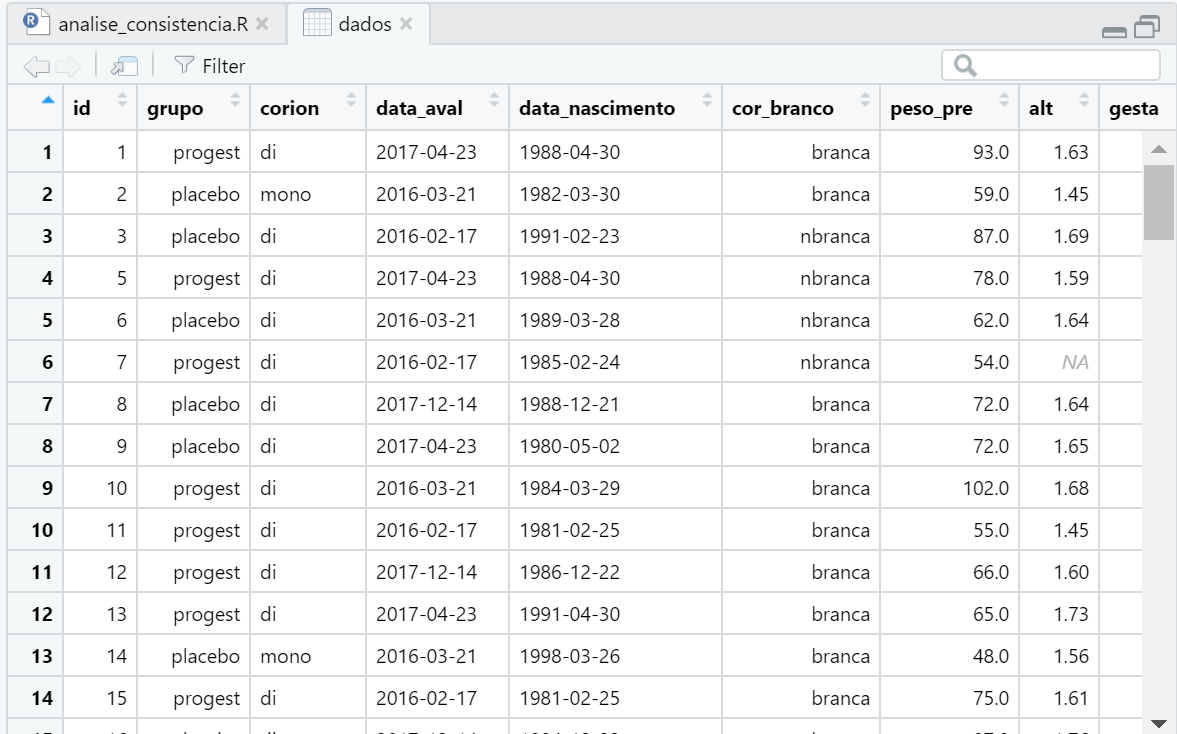
\includegraphics[width=1\linewidth]{figures/print-tela} \caption{Tela dos dados após comando View(dados)}\label{fig:view}
\end{figure}

Finalmente chegamos nas variáveis quantitativas. Uma forma de identificar problemas em variáveis quantitativas é avaliar os valores mínimo e máximo de cada variável e ver se tem algum valor impossível para a mesma.

Veja que tem uma altura de 163. A unidade de medida é em metros e a altura em questão foi um erro de digitação.
O certo era 1.63. Então vamos primeiro identificar o caso e depois vamos corrigir.

\begin{Shaded}
\begin{Highlighting}[]
\NormalTok{dados[dados}\OperatorTok{$}\NormalTok{alt}\OperatorTok{==}\DecValTok{163}\NormalTok{,]}
\end{Highlighting}
\end{Shaded}

\begin{verbatim}
## # A tibble: 3 x 20
##      id grupo corion data_aval  data_nascimento cor_branco peso_pre   alt gesta
##   <dbl> <fct> <fct>  <date>     <date>          <fct>         <dbl> <dbl> <dbl>
## 1    NA <NA>  <NA>   NA         NA              <NA>             NA    NA    NA
## 2    27 prog~ di     2016-02-17 1997-02-21      nbranca          58   163     1
## 3    NA <NA>  <NA>   NA         NA              <NA>             NA    NA    NA
## # ... with 11 more variables: para <dbl>, aborto <dbl>, ind_ap <fct>,
## #   tabagismo <fct>, alcool <fct>, drogas <fct>, ig_aval <dbl>,
## #   medida_colo <dbl>, num_contra_ctg <dbl>, igp_semana <dbl>, igp_dia <dbl>
\end{verbatim}

O caso em questão é o id=27 e vamos novamente usar a função \texttt{ifelse} para substituir o valorr:

\begin{Shaded}
\begin{Highlighting}[]
\NormalTok{dados}\OperatorTok{$}\NormalTok{alt <-}\StringTok{ }\KeywordTok{ifelse}\NormalTok{(dados}\OperatorTok{$}\NormalTok{id}\OperatorTok{==}\DecValTok{27}\NormalTok{,}\FloatTok{1.63}\NormalTok{,dados}\OperatorTok{$}\NormalTok{alt)}
\end{Highlighting}
\end{Shaded}

Há também um valor absurdo para ``ig\_aval'' (idade gestacional da avalição) de 83.86. Vamos identificar o id para depois corrigir:

\begin{Shaded}
\begin{Highlighting}[]
\NormalTok{dados[dados}\OperatorTok{$}\NormalTok{ig_aval}\OperatorTok{==}\FloatTok{83.86}\NormalTok{,]}
\end{Highlighting}
\end{Shaded}

\begin{verbatim}
## # A tibble: 1 x 20
##      id grupo corion data_aval  data_nascimento cor_branco peso_pre   alt gesta
##   <dbl> <fct> <fct>  <date>     <date>          <fct>         <dbl> <dbl> <dbl>
## 1    21 plac~ mono   2017-04-23 1988-04-30      branca           44  1.64     1
## # ... with 11 more variables: para <dbl>, aborto <dbl>, ind_ap <fct>,
## #   tabagismo <fct>, alcool <fct>, drogas <fct>, ig_aval <dbl>,
## #   medida_colo <dbl>, num_contra_ctg <dbl>, igp_semana <dbl>, igp_dia <dbl>
\end{verbatim}

Como podemos observar, o id=21 é o caso inconsistente para ``ig\_aval'' e o pesquisador checou que o correto é 33.86. Vamos então corrigir novamente com a função \texttt{ifelse}.

\begin{Shaded}
\begin{Highlighting}[]
\NormalTok{dados}\OperatorTok{$}\NormalTok{ig_aval <-}\StringTok{ }\KeywordTok{ifelse}\NormalTok{(dados}\OperatorTok{$}\NormalTok{id}\OperatorTok{==}\DecValTok{21}\NormalTok{,}\FloatTok{33.86}\NormalTok{,dados}\OperatorTok{$}\NormalTok{ig_aval)}
\end{Highlighting}
\end{Shaded}

Agora está tudo certo?

\begin{Shaded}
\begin{Highlighting}[]
\NormalTok{skimr}\OperatorTok{::}\KeywordTok{skim}\NormalTok{(dados)}
\end{Highlighting}
\end{Shaded}

\begin{verbatim}
## Error in kable_latex(x = structure(c("Name", "Number of rows", "Number of columns", : unused argument (table.attr = "style='width: auto;'\n        class='table table-condensed'")
\end{verbatim}

\hypertarget{transformauxe7uxe3o-dos-dados}{%
\section{Transformação dos dados}\label{transformauxe7uxe3o-dos-dados}}

Nessa parte do material discutiremos como fazer algumas transformações úteis nas variáveis. Para isso, utilizaremos as funções do pacote \texttt{dplyr}, um pacote bastante útil para a manipulação de dados.

\hypertarget{transformauxe7uxe3o-de-variuxe1veis-quantitativas}{%
\subsection{Transformação de variáveis quantitativas}\label{transformauxe7uxe3o-de-variuxe1veis-quantitativas}}

Primeiramente, temos o interesse em criar a variável IMC, dada pelo peso (em kg) dividido pela altura (em metros) ao quadrado. Para isso, usamos a função \texttt{mutate} do \texttt{dplyr}:

\begin{Shaded}
\begin{Highlighting}[]
\NormalTok{dados <-}\StringTok{ }\NormalTok{dplyr}\OperatorTok{::}\KeywordTok{mutate}\NormalTok{(dados,}\DataTypeTok{imc =}\NormalTok{ peso_pre}\OperatorTok{/}\NormalTok{(alt}\OperatorTok{^}\DecValTok{2}\NormalTok{))}
\end{Highlighting}
\end{Shaded}

Vamos ver então como ficou:

\begin{Shaded}
\begin{Highlighting}[]
\NormalTok{skimr}\OperatorTok{::}\KeywordTok{skim}\NormalTok{(dados}\OperatorTok{$}\NormalTok{imc) }\CommentTok{#coloquei só imc para só fazer descritivas para imc.}
\end{Highlighting}
\end{Shaded}

\begin{verbatim}
## Error in kable_latex(x = structure(c("Name", "Number of rows", "Number of columns", : unused argument (table.attr = "style='width: auto;'\n        class='table table-condensed'")
\end{verbatim}

Note que há três valores ausentes para ``imc'', uma vez que há dois valores ausentes para ``alt'' e outro para ``peso\_pre''.

Observe que na planilha tem duas colunas sobre idade gestacional: igp\_semanas (idade gestacional em semanas fechadas) e igp\_dia (dias ainda não de 1 semana completa). Vamos criar uma coluna que combine essas duas informações e que transforme os dias em semanas de maneira fracionada.

\begin{Shaded}
\begin{Highlighting}[]
\NormalTok{dados <-}\StringTok{ }\NormalTok{dplyr}\OperatorTok{::}\KeywordTok{mutate}\NormalTok{(dados,}\DataTypeTok{igp =}\NormalTok{ igp_semana}\OperatorTok{+}\NormalTok{igp_dia}\OperatorTok{/}\DecValTok{7}\NormalTok{)}
\end{Highlighting}
\end{Shaded}

Vamos ver então como ficou:

\begin{Shaded}
\begin{Highlighting}[]
\NormalTok{skimr}\OperatorTok{::}\KeywordTok{skim}\NormalTok{(dados}\OperatorTok{$}\NormalTok{igp) }\CommentTok{#coloquei só igp para só fazer descritivas para igp.}
\end{Highlighting}
\end{Shaded}

\begin{verbatim}
## Error in kable_latex(x = structure(c("Name", "Number of rows", "Number of columns", : unused argument (table.attr = "style='width: auto;'\n        class='table table-condensed'")
\end{verbatim}

\hypertarget{transformauxe7uxe3o-de-variuxe1veis-qualitativas}{%
\subsection{Transformação de variáveis qualitativas}\label{transformauxe7uxe3o-de-variuxe1veis-qualitativas}}

A variável ``gesta'' indica o número de gestações, contando com a atual da gestante em gestão. Logo, uma gestante com gesta=1 está em sua primeira gestação, ou seja, é primigesta. Queremos criar uma nova variável indicadora de gestação primigesta. Há diferentes forma de fazer isso. Vamos usar o comando \texttt{ifelse} já utilizado anteriormente:

\begin{Shaded}
\begin{Highlighting}[]
\NormalTok{dados}\OperatorTok{$}\NormalTok{primigesta <-}\StringTok{ }\KeywordTok{ifelse}\NormalTok{(dados}\OperatorTok{$}\NormalTok{gesta}\OperatorTok{==}\DecValTok{1}\NormalTok{,}\DecValTok{1}\NormalTok{,}\DecValTok{0}\NormalTok{)}
\end{Highlighting}
\end{Shaded}

Agora vamos recodificar primigesta com o nome de cada categoria:

\begin{Shaded}
\begin{Highlighting}[]
\NormalTok{dados}\OperatorTok{$}\NormalTok{primigesta <-}\StringTok{ }\KeywordTok{as.factor}\NormalTok{(dados}\OperatorTok{$}\NormalTok{primigesta)}
\NormalTok{dados}\OperatorTok{$}\NormalTok{primigesta <-}\StringTok{ }\NormalTok{forcats}\OperatorTok{::}\KeywordTok{fct_recode}\NormalTok{(dados}\OperatorTok{$}\NormalTok{primigesta,}
                                \DataTypeTok{nao =} \StringTok{"0"}\NormalTok{, }
                                \DataTypeTok{sim =} \StringTok{"1"}\NormalTok{)}
\end{Highlighting}
\end{Shaded}

Outra variável qualitativa que é função de uma variável quantitativa da planilha é a prematuridade. Definimos aqui prematuridade se idade gestacional do parto for menor que 37 semanas.

\begin{Shaded}
\begin{Highlighting}[]
\NormalTok{dados}\OperatorTok{$}\NormalTok{prematuridade <-}\StringTok{ }\KeywordTok{ifelse}\NormalTok{(dados}\OperatorTok{$}\NormalTok{igp}\OperatorTok{<}\DecValTok{37}\NormalTok{,}\DecValTok{1}\NormalTok{,}\DecValTok{0}\NormalTok{)}
\end{Highlighting}
\end{Shaded}

Agora vamos recodificar ``prematuridade'' com o nome de cada categoria:

\begin{Shaded}
\begin{Highlighting}[]
\NormalTok{dados}\OperatorTok{$}\NormalTok{prematuridade <-}\StringTok{ }\KeywordTok{as.factor}\NormalTok{(dados}\OperatorTok{$}\NormalTok{prematuridade)}
\NormalTok{dados}\OperatorTok{$}\NormalTok{prematuridade <-}\StringTok{ }\NormalTok{forcats}\OperatorTok{::}\KeywordTok{fct_recode}\NormalTok{(dados}\OperatorTok{$}\NormalTok{prematuridade,}
                                \DataTypeTok{nao =} \StringTok{"0"}\NormalTok{, }
                                \DataTypeTok{sim =} \StringTok{"1"}\NormalTok{)}
\end{Highlighting}
\end{Shaded}

Vamos ver então como ficou:

\begin{Shaded}
\begin{Highlighting}[]
\NormalTok{skimr}\OperatorTok{::}\KeywordTok{skim}\NormalTok{(dados,primigesta,prematuridade) }
\end{Highlighting}
\end{Shaded}

\begin{verbatim}
## Error in kable_latex(x = structure(c("Name", "Number of rows", "Number of columns", : unused argument (table.attr = "style='width: auto;'\n        class='table table-condensed'")
\end{verbatim}

Veja que coloquei ``primigesta'' e ``prematuridade'' no segundo e terceiro argumento do \texttt{skim}para apenas retornar as descritivas dessas duas variáveis.

\textbf{Exercício}:

\begin{enumerate}
\def\labelenumi{\arabic{enumi})}
\item
  Crie a variável indicador\_aborto (sim e nao) - sim se aborto \textgreater=1 e nao se aborto=0.
\item
  Crie a variável primipara (sim e nao) - sim se para \textgreater=1 e nao se para=0.
\end{enumerate}

\hypertarget{manipulauxe7uxe3o-de-datas}{%
\subsection{Manipulação de datas}\label{manipulauxe7uxe3o-de-datas}}

Na base de dados, há duas variáveis de data: data da avaliação e data do nascimento. A diferença entre as duas datas, em anos, é a idade da gestante no momento da avaliação. Para realizar operações com data, usaremos o pacote \texttt{lubridate}.

A data está salva no formato ano-mês-dia e por isso usamos a função \texttt{ymd(.)} para as variáveis de data. Para calcular a diferença entre as data, usamos a função \(%--%
\), atribuindo ao objeto intervalo. Por fim, obtemos a idade ao dividir o intervalo por ano.

\begin{Shaded}
\begin{Highlighting}[]
\NormalTok{intervalo <-}\StringTok{ }\NormalTok{lubridate}\OperatorTok{::}\KeywordTok{ymd}\NormalTok{(dados}\OperatorTok{$}\NormalTok{data_nascimento) }
\OperatorTok\StringTok{  }\NormalTok{lubridate}\OperatorTok{::}\KeywordTok{ymd}\NormalTok{(dados}\OperatorTok{$}\NormalTok{data_aval)}
\NormalTok{dados}\OperatorTok{$}\NormalTok{idade <-}\StringTok{ }\NormalTok{intervalo }\OperatorTok{/}\StringTok{ }\NormalTok{lubridate}\OperatorTok{::}\KeywordTok{dyears}\NormalTok{(}\DecValTok{1}\NormalTok{)  }\CommentTok{#número de anos}
\NormalTok{dados}\OperatorTok{$}\NormalTok{idade <-}\StringTok{ }\KeywordTok{trunc}\NormalTok{(dados}\OperatorTok{$}\NormalTok{idade) }\CommentTok{#usamos a idade completada }
\end{Highlighting}
\end{Shaded}

\begin{verbatim}
## Error: <text>:2:1: SPECIAL inesperado
## 1: intervalo <- lubridate::ymd(dados$data_nascimento) 
## 2: %--%
##    ^
\end{verbatim}

A última linha do código acima utiliza a função \texttt{trunc} para truncar a idade para não usar a fração dos meses da idade ainda não completa e sim usar a idade completada no último aniversário.

Vale ressaltar que há várias funções importantes para lidar com variáveis de data no pacote \texttt{lubridate}. Para mais detalhes, ver a \href{https://cran.r-project.org/web/packages/lubridate/vignettes/lubridate.html}{documentação do lubridate}.

\hypertarget{filtragem-de-observauxe7uxf5es}{%
\subsection{Filtragem de observações}\label{filtragem-de-observauxe7uxf5es}}

Uma função bastante importante quando estamos analisando dados é filtrar de acordo com uma condição de interesse. Suponha que temos interesse em realizar uma determinada análise apenas com gestantes com menos de 23 anos. Para selecionar apenas as gestantes mais novas, podemos utilizar a função \texttt{filter} do pacote \texttt{dplyr}.

\begin{Shaded}
\begin{Highlighting}[]
\NormalTok{dados_jovens <-}\StringTok{ }\KeywordTok{filter}\NormalTok{(dados,idade}\OperatorTok{<}\DecValTok{23}\NormalTok{)}
\end{Highlighting}
\end{Shaded}

\begin{verbatim}
## Error: Problem with `filter()` input `..1`.
## x objeto 'idade' não encontrado
## i Input `..1` is `idade < 23`.
\end{verbatim}

Veja que agora o objeto dados\_jovens é a base de dados apenas com aquelas cuja idade é menor que 23 (use o comando View(dados\_jovens) para verificar).

Utilizando os operadores lógicos ``\&'' (e) e ``\textbar{}'' (ou), conseguimos realizar algumas condições, como mostrado no exemplo abaixo.

Agora, queremos selecionar apenas as gestantes mais novas e do grupo progesterona. Para isso:

\begin{Shaded}
\begin{Highlighting}[]
\NormalTok{dados_jovens_progest <-}\StringTok{  }\KeywordTok{filter}\NormalTok{(dados,idade}\OperatorTok{<}\DecValTok{23} \OperatorTok{&}\StringTok{ }\NormalTok{grupo}\OperatorTok{==}\StringTok{"progest"}\NormalTok{)}
\end{Highlighting}
\end{Shaded}

\begin{verbatim}
## Error: Problem with `filter()` input `..1`.
## x objeto 'idade' não encontrado
## i Input `..1` is `idade < 23 & grupo == "progest"`.
\end{verbatim}

Acho que aqui vale uma nota sobre o pacote \texttt{dplyr} e por isso dediquei uma subseção para ele, no que segue.

\hypertarget{pacote-dplyr}{%
\subsubsection{Pacote dplyr}\label{pacote-dplyr}}

O \texttt{\{dplyr\}} é um pacote muito útil para realizar transformação de dados.

Suas principais funções são:

\begin{itemize}
\item
  filter() - filtra linhas;
\item
  select() - seleciona colunas;
\item
  arrange() - ordena a base;
\item
  mutate() - cria/modifica colunas.
\end{itemize}

Já falamos das funções \texttt{filter} e \texttt{mutate} anteriormente, então falamos brevemente das outras funções no que segue.

A função \texttt{select()} seleciona colunas (variáveis). Vamos supor que eu tenha interesse em criar um objeto com só as variáveis ``id'', ``grupo'', ``prematuridade''.

\begin{Shaded}
\begin{Highlighting}[]
\NormalTok{dados_s <-}\StringTok{ }\NormalTok{dplyr}\OperatorTok{::}\KeywordTok{select}\NormalTok{(dados,id, grupo, prematuridade)}
\end{Highlighting}
\end{Shaded}

Veja em \texttt{View(dados\_s)} que essa base de dados só contém as colunas selecionadas.

Sempre quando queremos retirar algo do banco de dados, colocamos um ``-'' antes da variável. No exemplo abaixo, queremos rerirar ``igp\_semana'' e ``igp\_dia''.

\begin{Shaded}
\begin{Highlighting}[]
\NormalTok{dados_s1 <-}\StringTok{ }\NormalTok{dplyr}\OperatorTok{::}\KeywordTok{select}\NormalTok{(dados,}\OperatorTok{-}\NormalTok{igp_semana,}\OperatorTok{-}\NormalTok{igp_dia)}
\end{Highlighting}
\end{Shaded}

Veja em \texttt{View(dados\_s1)} que essa base de dados só contém as colunas selecionadas.

Com a função \texttt{arrange()}, conseguimos ordenar a base de acordo com uma ou mais colunas. Para gerar uma ordem descescente de alguma variável, utilizamos a função \texttt{desc} como segue:

\begin{Shaded}
\begin{Highlighting}[]
\NormalTok{dados_cres <-}\StringTok{ }\NormalTok{dplyr}\OperatorTok{::}\KeywordTok{arrange}\NormalTok{(dados,alt)}
\end{Highlighting}
\end{Shaded}

\begin{Shaded}
\begin{Highlighting}[]
\NormalTok{dados_decres <-}\StringTok{ }\NormalTok{dplyr}\OperatorTok{::}\KeywordTok{arrange}\NormalTok{(dados,}\KeywordTok{desc}\NormalTok{(alt))}
\end{Highlighting}
\end{Shaded}

No primeiro código acima, ordenamos a planilha em ordem crescente pela altura. Já no segundo código, ordenamos a planilha em ordem decrescente pela altura (a primeira observação na planilha dados\_decres é aquela cuja gestante é a mais alta).

\hypertarget{exercuxedcios}{%
\section{Exercícios}\label{exercuxedcios}}

\hypertarget{teuxf3ricos}{%
\subsection{Teóricos}\label{teuxf3ricos}}

\begin{enumerate}
\def\labelenumi{\arabic{enumi}.}
\item
  Por que é importante ter a população bem definida?
\item
  Por que é importante pensar em todo planejamento amostral ao
  invés de pensar apenas no cálculo do tamanho amostral?
\item
  O que é uma variável confundidora?
\item
  Classifique as seguintes variáveis:
\end{enumerate}

\begin{enumerate}
\def\labelenumi{\alph{enumi}.}
\item
  Sexo
\item
  Altura
\item
  Peso
\item
  Fuma (sim ou não)
\item
  Tolerância ao cigarro (indiferente, incomoda pouco, incomoda muito)
\item
  Consumo de café (nunca, 1 a 2 vezes por semana, 3 a 6 vezes por semana, uma vez por dia, \(>\) 1 vez por dia)
\item
  Horas de atividade física por semana
\end{enumerate}

\hypertarget{pruxe1ticos-no-r}{%
\subsection{Práticos no R}\label{pruxe1ticos-no-r}}

\begin{enumerate}
\def\labelenumi{\arabic{enumi}.}
\setcounter{enumi}{4}
\tightlist
\item
  Considere a base de dados ``dados\_gemelares'':
\end{enumerate}

\begin{enumerate}
\def\labelenumi{\alph{enumi}.}
\item
  Crie a variável igp (idade gestacional do parto)
  obtida ao somar igp\_semana e igp\_dia/7.
\item
  Crie a variável indicador\_aborto (sim e não) - sim se aborto \textgreater=1 e não se aborto=0.
\item
  Crie a variável primipara (sim e não) - não se para \textgreater=1 e sim se para=0.
\item
  Obtenha uma nova base de dados ao considerar só os casos primigestas (note que queremos filtrar quem é primigesta=sim).
\item
  Obtenha uma nova base de dados ao considerar só os casos que não fumam e não fazem uso de álcool.
\end{enumerate}

\begin{enumerate}
\def\labelenumi{\arabic{enumi}.}
\setcounter{enumi}{5}
\tightlist
\item
  Considere agora a base de dados ``dados\_gemelares\_2''. Realize uma análise de consistência similar a que realizamos para a base de dados ``dados\_gemelares'' na Seção \ref{consistencia}.
\end{enumerate}

\hypertarget{anuxe1lise-exploratuxf3ria-dos-dados}{%
\chapter{Análise exploratória dos dados}\label{anuxe1lise-exploratuxf3ria-dos-dados}}

Neste capítulo consideramos a análise descritiva das variáveis da base de dados de interesse.

A análise descritiva pode ser vista como o conjunto de técnicas numéricas e gráficas utilizadas para detectar padrões, resumir informação e apresentar visivelmente características de um conjunto de dados. Assim, podemos identificar \citep{morettin2020introduccaoa}:

\begin{enumerate}
\def\labelenumi{\roman{enumi})}
\item
  qual a frequência com que cada valor aparece no conjunto de dados ou seja, qual a distribuição de frequências dos
  dados?
\item
  quais são alguns valores típicos do conjunto de dados, como mínimo e máximo?
\item
  qual seria um valor para representar a posição (ou localização) central do conjunto de dados?
\item
  qual seria uma medida da variabilidade ou dispersão dos dados?
\item
  existem valores atípicos ou discrepantes (\emph{outliers}) no conjunto de dados?
\item
  os dados podem ser considerados simétricos?
\end{enumerate}

Para isso, utilizamos:

\begin{itemize}
\tightlist
\item
  tabelas de frequências;
\item
  medidas para resumir os dados;
\item
  gráficos.
\end{itemize}

As técnicas empregadas na análise descritiva dependem do tipo de variáveis que compõem o conjunto de dados em questão. Por isso, recomendo que reveja a Seção \ref{variaveis} sobre os tipos de variáveis.

\hypertarget{tabelas-de-frequuxeancias}{%
\section{Tabelas de frequências}\label{tabelas-de-frequuxeancias}}

Uma tabela contendo as frequências absolutas (número de casos) e/ou relativas (número de casos relativo ao total) para cada categoria da variável qualitativa é chamada de distribuição de frequências dessa variável.

Ao considerar a base de dados de gestações gemelares, vamos contruir uma tabela de frequências para a variável ``prematuridade''. No R, há diversar maneiras de obter uma tabela de frequências. Vamos utilizar aqui a função \texttt{freq} do pacote \texttt{summarytools}.

\begin{Shaded}
\begin{Highlighting}[]
\KeywordTok{library}\NormalTok{(summarytools)}
\end{Highlighting}
\end{Shaded}

\begin{Shaded}
\begin{Highlighting}[]
\NormalTok{summarytools}\OperatorTok{::}\KeywordTok{freq}\NormalTok{(dados}\OperatorTok{$}\NormalTok{prematuridade,}\DataTypeTok{cumul=}\OtherTok{FALSE}\NormalTok{)}
\end{Highlighting}
\end{Shaded}

\begin{verbatim}
## Frequencies  
## 
##               Freq   % Valid   % Total
## ----------- ------ --------- ---------
##         nao     44     42.31     42.31
##         sim     60     57.69     57.69
##        <NA>      0                0.00
##       Total    104    100.00    100.00
\end{verbatim}

Pela tabela acima, observamos que quase 58\% dos nascimentos gemelares foram prematuros e que não há observações faltantes para essa variável (linha \(<NA>\) está vazia). Caso queira que não apareça na tabela a linha com dados faltantes, só é necessário acrescentar o argumento \texttt{report.nas\ =FALSE} na função, como segue:

\begin{Shaded}
\begin{Highlighting}[]
\NormalTok{summarytools}\OperatorTok{::}\KeywordTok{freq}\NormalTok{(dados}\OperatorTok{$}\NormalTok{prematuridade,}\DataTypeTok{cumul=}\OtherTok{FALSE}\NormalTok{,}
                   \DataTypeTok{report.nas=}\OtherTok{FALSE}\NormalTok{)}
\end{Highlighting}
\end{Shaded}

\begin{verbatim}
## Frequencies  
## 
##               Freq        %
## ----------- ------ --------
##         nao     44    42.31
##         sim     60    57.69
##       Total    104   100.00
\end{verbatim}

Observe também que colocamos o argumento \texttt{cumul=FALSE}, indicando que não temos interesse em acrescentar na tabela a coluna com as frequências relativas acumuladas. Essa coluna é útil quando a variável é qualitativa ordinal, o que não é o caso da prematuridade.

Outra dica importante é utilizar a função \texttt{view} (dessa vez tudo minúsculo). Veja que, ao utilizar \texttt{view(freq(dados\$prematuridade,cumul=FALSE,report.nas=FALSE))} a tabela aparecerá mais bonita no menu ``Viewer'' do RStudio. Dali você pode copiar para o destino de interesse.

\hypertarget{medidas-resumo}{%
\section{Medidas resumo}\label{medidas-resumo}}

Se utilizarmos uma tabela de frequências para uma variável quantitativas (especialmente no caso de variáveis contínuas), obteríamos frequências muito pequenas (em geral 1) para os diversos valores da variável, deixando de atingir o objetivo de resumir os dados.

Nesse sentido, apresentamos aqui medidas resumo que podem ser utilizadas para variáveis quantitativas. Essas serão divididas entre medidas de posição e medidas de dispersão.

\hypertarget{medidas-de-posiuxe7uxe3o}{%
\subsection{Medidas de posição}\label{medidas-de-posiuxe7uxe3o}}

As medidas de posição, como o nome diz, indicam posições de interesse da variável. Consideramos aqui as seguintes medidas: valor mínimo, valor máximo, moda, média, mediana e percentis.

O \textbf{mínimo} é o menor valor observado e \textbf{máximo} é o maior valor observado.

A moda, a média e a mediana são todas \textbf{medidas de posição central}: medidas que buscam descrever um valor típico que a variável tende a apresentar.

A \textbf{moda} é o(s) valor(es) mais frequente(s). Vale citar que a moda também pode ser usada para variáveis qualitativas.

A \textbf{média} é a medida obtida ao somar todos os valores da variável dividida pelo número de observações. Podemos interpretar a média como sendo um ponto de equilíbrio: os valores da variáveis são representadas como pesos de mesma massa posicionados sobre uma reta de massa desprezível nas posições referentes aos valores da variável em questão.

Já a \textbf{mediana} divide os dados de forma que 50\% deles são menores e 50\% deles são maiores que a mediana.

Para considerar dados de posição não centrais, podemos citar os quantis. Um quantil de ordem p é um valor da variável que deixa \(100p\%\) \((0 < p < 1)\) das observações a sua esquerda, ou seja, são menores que ele.

São alguns quantis conhecidos:

\begin{itemize}
\item
  \textbf{Percentis} - valores inteiros de \(100p\%\). O percentil 20, por exemplo, é o valor da variável que 20\% das observações apresentam menor que ele.
\item
  \textbf{Decis} - dados divididos em 10 partes iguais. O primeiro decil, por exemplo, é o percentil 10 e o sexto decil é o percentil 60.
\item
  \textbf{Quartis} - dados divididos em 4 partes iguais. O primeiro quartil é o percentil 25, o segundo quartil é o percentil 50 e o terceiro quartil é o percentil 75.
  Vale notar que o segundo quartil é a mediana.
\end{itemize}

\hypertarget{medidas-de-dispersuxe3o}{%
\subsection{Medidas de dispersão}\label{medidas-de-dispersuxe3o}}

As medidas de dispersão são valores que quantificam quão dispersos os dados são. Consideramos aqui as seguintes medidas: amplitude, intervalo interquartil, variância e desvio padrão.

A \textbf{amplitude} é a diferença entre o valor máximo e o valor mínimo. O \textbf{intervalo interquartil} é a diferença entre o terceiro e o primeiro quartil, ou seja, é a amplitude entre os 50\% dos dados centrais.

Queremos uma medida de dispersão que não considere apenas dois valores da amostra (mínimo e máximo ou primeiro e terceiro quartis) e sim todos os dados. Uma medida bastante intuitiva seria considerar a soma dos desvios das observações em torno da média. Mas aí temos um problema: a soma dos desvios da média é sempre zero! Isso acontece porque sempre há desvios positivos e negativos que se anulam. Uma solução para essa questão é considerar alguma função que considere apenas o valor do desvio e não o seu sinal. Uma função candidata é a função quadrática (lembre que, por exemplo, \((-2)^2=4\)). Nessa construção surge a \textbf{variância}: soma dos desvios quadrados dividida pelo total de observações, ou seja, a média dos desvios quadrados. Assim, a variância quantifica o quanto os dados estão dispersos da média, em média.

Como a unidade de medida da variância é o quadrado da unidade de medida da variável correspondente, convém definir outra medida de dispersão que mantenha a unidade de medida original. Uma medida com essa propriedade é a raiz quadrada da variância, conhecida por \textbf{desvio padrão}.

No R, para obter essas medidas resumo vamos utilizar a função \texttt{descr} também do pacote \texttt{summarytools}. No comando abaixo pedimos ao R as medidas descritivas da variável quantitativa ``medida\_colo''.

\begin{Shaded}
\begin{Highlighting}[]
\KeywordTok{descr}\NormalTok{(dados}\OperatorTok{$}\NormalTok{medida_colo)}
\end{Highlighting}
\end{Shaded}

\begin{verbatim}
## Descriptive Statistics  
## value  
## N: 104  
## 
##                      value
## ----------------- --------
##              Mean    24.67
##           Std.Dev     9.93
##               Min     2.70
##                Q1    17.90
##            Median    24.75
##                Q3    33.05
##               Max    46.30
##               MAD    11.27
##               IQR    15.07
##                CV     0.40
##          Skewness    -0.03
##       SE.Skewness     0.24
##          Kurtosis    -0.74
##           N.Valid   104.00
##         Pct.Valid   100.00
\end{verbatim}

Veja que a função retorna outras medidas resumo além daquelas citadas anteriormente. Se quiser uma tabela com algumas medidas resumo, podemos informar ao R por meio do argumento \texttt{stats}. Ainda, se quisermos que na tabela as medidas resumo fiquem na coluna, usamos o argumento \texttt{transpose\ =\ TRUE}, como segue:

\begin{Shaded}
\begin{Highlighting}[]
\KeywordTok{descr}\NormalTok{(dados}\OperatorTok{$}\NormalTok{medida_colo,}\DataTypeTok{stats =} \KeywordTok{c}\NormalTok{(}\StringTok{"min"}\NormalTok{, }\StringTok{"mean"}\NormalTok{, }\StringTok{"med"}\NormalTok{,}\StringTok{"sd"}\NormalTok{,}\StringTok{"max"}\NormalTok{),}
      \DataTypeTok{transpose =} \OtherTok{TRUE}\NormalTok{) }\CommentTok{#sd é o desvio padrão}
\end{Highlighting}
\end{Shaded}

\begin{verbatim}
## Descriptive Statistics  
## value  
## N: 104  
## 
##                Min    Mean   Median   Std.Dev     Max
## ----------- ------ ------- -------- --------- -------
##       value   2.70   24.67    24.75      9.93   46.30
\end{verbatim}

Outro pacote bastante interessante para medidas descritivas é o \texttt{modelsummary}. Destacamos algumas funções desse pacote:

\begin{itemize}
\item
  \texttt{datasummary\_skim}: retorna as medidas descritivas das variáveis do banco de dados a depender do tipo identificado no argumento \texttt{type=} (categorical ou numeric);
\item
  \texttt{datasummary}: retorna as medidas descritivas das variáveis a depender de como monta os argumentos da função, permitindo retornar as medidas descritivas das variáveis quantitativas de interesse por categorias de outra(s) variável(is).
\end{itemize}

\begin{Shaded}
\begin{Highlighting}[]
\KeywordTok{library}\NormalTok{(modelsummary)}
\end{Highlighting}
\end{Shaded}

Ao usar a função \texttt{datasummary\_skim}, vamos obter as medidas descritivas das variáveis quantitativas (argumento \texttt{type\ =\ "numeric"}) e das variáveis qualitativas (argumento \texttt{type\ =\ "categorical"}), respectivamente:

\begin{Shaded}
\begin{Highlighting}[]
\KeywordTok{datasummary_skim}\NormalTok{(}
\NormalTok{  dados,}
  \DataTypeTok{type =} \StringTok{"numeric"}\NormalTok{,}
  \DataTypeTok{histogram =} \OtherTok{FALSE}
\NormalTok{)}
\end{Highlighting}
\end{Shaded}

\begin{Shaded}
\begin{Highlighting}[]
\KeywordTok{datasummary_skim}\NormalTok{(}
\NormalTok{  dados,}
  \DataTypeTok{type =} \StringTok{"categorical"}
\NormalTok{)}
\end{Highlighting}
\end{Shaded}

Agora vamos comentar sobre a função mais interessante desse pacote, a função \texttt{datasummary}. Suponha que eu tenho interesse em obter as medidas descritivas das variáveis ``igp'', ``idade'', ``imc'', ``medida\_colo'' e ``num\_contra\_ctg'' por grupo (progesterona ou placebo), apresentando as seguintes medidas descritivas: média, mediana, desvio padrão, mínimo, máximo e tamanho da amostra válido (sem considerar observações faltantes para a variável em questão).

\begin{Shaded}
\begin{Highlighting}[]
\CommentTok{### Essas funcoes abaixo são auxiliares para calcular as descritivas}
\CommentTok{#em cenário de presença de dados faltantes}
\NormalTok{media <-}\StringTok{ }\ControlFlowTok{function}\NormalTok{(x) }\KeywordTok{mean}\NormalTok{(x, }\DataTypeTok{na.rm =} \OtherTok{TRUE}\NormalTok{)}
\NormalTok{medi <-}\StringTok{ }\ControlFlowTok{function}\NormalTok{(x) }\KeywordTok{median}\NormalTok{(x, }\DataTypeTok{na.rm =} \OtherTok{TRUE}\NormalTok{)}
\NormalTok{dp <-}\StringTok{ }\ControlFlowTok{function}\NormalTok{(x) }\KeywordTok{sd}\NormalTok{(x, }\DataTypeTok{na.rm =} \OtherTok{TRUE}\NormalTok{)}
\NormalTok{mini <-}\StringTok{ }\ControlFlowTok{function}\NormalTok{(x) }\KeywordTok{min}\NormalTok{(x, }\DataTypeTok{na.rm =} \OtherTok{TRUE}\NormalTok{)}
\NormalTok{maxi <-}\StringTok{ }\ControlFlowTok{function}\NormalTok{(x) }\KeywordTok{max}\NormalTok{(x, }\DataTypeTok{na.rm =} \OtherTok{TRUE}\NormalTok{)}
\NormalTok{n <-}\StringTok{ }\ControlFlowTok{function}\NormalTok{(x) }\KeywordTok{sum}\NormalTok{(}\OperatorTok{!}\KeywordTok{is.na}\NormalTok{(x))}
\end{Highlighting}
\end{Shaded}

\begin{Shaded}
\begin{Highlighting}[]
\KeywordTok{datasummary}\NormalTok{((igp}\OperatorTok{+}\NormalTok{idade}\OperatorTok{+}\NormalTok{imc}\OperatorTok{+}\NormalTok{medida_colo}\OperatorTok{+}\NormalTok{num_contra_ctg)}\OperatorTok{~}
\StringTok{              }\NormalTok{grupo}\OperatorTok{*}\NormalTok{(n}\OperatorTok{+}\NormalTok{media}\OperatorTok{+}\NormalTok{dp}\OperatorTok{+}\NormalTok{mini}\OperatorTok{+}\NormalTok{medi}\OperatorTok{+}\NormalTok{maxi), }\DataTypeTok{data =}\NormalTok{ dados)}
\end{Highlighting}
\end{Shaded}

Agora veja como fica se eu considerar as medidas descritivas das variáveis quantitativas por duas variáveis qualitativas:

\begin{Shaded}
\begin{Highlighting}[]
\KeywordTok{datasummary}\NormalTok{(primigesta}\OperatorTok{*}\NormalTok{grupo}\OperatorTok{~}\NormalTok{(igp}\OperatorTok{+}\NormalTok{idade}\OperatorTok{+}\NormalTok{imc}\OperatorTok{+}\NormalTok{medida_colo}\OperatorTok{+}
\StringTok{  }\NormalTok{num_contra_ctg)}\OperatorTok{*}\NormalTok{(n}\OperatorTok{+}\NormalTok{media}\OperatorTok{+}\NormalTok{dp}\OperatorTok{+}\NormalTok{mini}\OperatorTok{+}\NormalTok{medi}\OperatorTok{+}\NormalTok{maxi), }\DataTypeTok{data =}\NormalTok{ dados)}
\end{Highlighting}
\end{Shaded}

Para mais detalhes sobre as medidas descritivas veja o Capítulo 3 de Morettin e Singer \citep{morettin2020introduccaoa}.

\hypertarget{tabelas-cruzadas---duas-variuxe1veis-qualitativas}{%
\section{Tabelas cruzadas - duas variáveis qualitativas}\label{tabelas-cruzadas---duas-variuxe1veis-qualitativas}}

Tabelas cruzadas ou tabelas de contingência são tabelas que apresentam frequências de duas variáveis qualitativas conjuntamente.

No R, para obter tabelas cruzadas vamos utilizar a função \texttt{ctable} também do pacote \texttt{summarytools}. No comando abaixo pedimos ao R uma tabela cruzada entre as variáveis qualitativas ``grupo'' e ``prematuridade''.

\begin{Shaded}
\begin{Highlighting}[]
\KeywordTok{ctable}\NormalTok{(dados}\OperatorTok{$}\NormalTok{grupo,}\DataTypeTok{y=}\NormalTok{dados}\OperatorTok{$}\NormalTok{prematuridade,}\DataTypeTok{prop=}\StringTok{"t"}\NormalTok{)}
\end{Highlighting}
\end{Shaded}

\begin{verbatim}
## Cross-Tabulation, Total Proportions  
## dados$grupo * dados$prematuridade  
## 
## ------------- --------------------- ------------ ------------ --------------
##                 dados$prematuridade          nao          sim          Total
##   dados$grupo                                                               
##       placebo                         19 (18.3%)   33 (31.7%)    52 ( 50.0%)
##       progest                         25 (24.0%)   27 (26.0%)    52 ( 50.0%)
##         Total                         44 (42.3%)   60 (57.7%)   104 (100.0%)
## ------------- --------------------- ------------ ------------ --------------
\end{verbatim}

No argumento \texttt{prop=} indica como será o cálculo das porcentagens apresentadas entre parênteses. Se o interesse for a porcentagem com relação ao total, o argumento é \texttt{prop="t"}. Se você desejar que a porcentagem seja calculada com relação às categorias da variável que está na linha é \texttt{prop="r"}:

\begin{Shaded}
\begin{Highlighting}[]
\KeywordTok{ctable}\NormalTok{(dados}\OperatorTok{$}\NormalTok{grupo,}\DataTypeTok{y=}\NormalTok{dados}\OperatorTok{$}\NormalTok{prematuridade,}\DataTypeTok{prop=}\StringTok{"r"}\NormalTok{)}
\end{Highlighting}
\end{Shaded}

\begin{verbatim}
## Cross-Tabulation, Row Proportions  
## dados$grupo * dados$prematuridade  
## 
## ------------- --------------------- ------------ ------------ --------------
##                 dados$prematuridade          nao          sim          Total
##   dados$grupo                                                               
##       placebo                         19 (36.5%)   33 (63.5%)    52 (100.0%)
##       progest                         25 (48.1%)   27 (51.9%)    52 (100.0%)
##         Total                         44 (42.3%)   60 (57.7%)   104 (100.0%)
## ------------- --------------------- ------------ ------------ --------------
\end{verbatim}

E, por fim, se for de interesse que a porcentagem seja calculada com relação às categorias da variável que está na coluna é \texttt{prop="c"}:

\begin{Shaded}
\begin{Highlighting}[]
\KeywordTok{ctable}\NormalTok{(dados}\OperatorTok{$}\NormalTok{grupo,}\DataTypeTok{y=}\NormalTok{dados}\OperatorTok{$}\NormalTok{prematuridade,}\DataTypeTok{prop=}\StringTok{"c"}\NormalTok{)}
\end{Highlighting}
\end{Shaded}

\begin{verbatim}
## Cross-Tabulation, Column Proportions  
## dados$grupo * dados$prematuridade  
## 
## ------------- --------------------- ------------- ------------- --------------
##                 dados$prematuridade           nao           sim          Total
##   dados$grupo                                                                 
##       placebo                         19 ( 43.2%)   33 ( 55.0%)    52 ( 50.0%)
##       progest                         25 ( 56.8%)   27 ( 45.0%)    52 ( 50.0%)
##         Total                         44 (100.0%)   60 (100.0%)   104 (100.0%)
## ------------- --------------------- ------------- ------------- --------------
\end{verbatim}

\hypertarget{gruxe1ficos}{%
\section{Gráficos}\label{gruxe1ficos}}

Um gráfico pode ser a maneira mais adequada para resumir e apresentar um conjunto de dados. Tem a vantagem de facilitar a compreensão de uma determinada situação que queira ser descrita, permitindo uma interpretação rápida e visual das suas principais características.

A visualização dos dados é uma etapa importantíssima da análise estatística, pois é também a partir dela que criamos a intuição necessária para escolher o teste ou modelo mais adequado para o nosso problema.

No Capítulo 3 do livro de Morettin e Singer também tem um conteúdo bastante interessante sobre gráficos e recomendamos sua leitura para a apresentação dos gráficos mais tradicionais em Estatística do ponto de vista mais teórico e, no que segue, discutimos como obter alguns gráficos no R.

\hypertarget{pacote-ggplot2}{%
\subsection{Pacote ggplot2}\label{pacote-ggplot2}}

Um pacote maravilhoso para gráficos no R é o \texttt{ggplot2}. A ideia por trás desse pacote é que o fato que um gráfico é um mapeamento dos dados a partir de atributos estéticos (cores, formas, tamanho) de formas geométricas (pontos, linhas, barras).

\begin{Shaded}
\begin{Highlighting}[]
\KeywordTok{library}\NormalTok{(ggplot2)}
\end{Highlighting}
\end{Shaded}

\textbf{Atributos estéticos}

A função \texttt{aes()} descreve como as variáveis são mapeadas em aspectos visuais (qual variável será representada no eixo x, qual será representada no eixo y, a cor e o tamanho dos componentes geométricos e etc) de formas geométricas definidas pelos geoms. Os aspectos que podem ou devem ser mapeados vão depender do tipo de gráfico que estamos querendo construir.

Aspectos visuais mais utilizados:

\begin{itemize}
\item
  color: altera a cor de formas que não têm área (pontos e retas);
\item
  fill: altera a cor de formas com área (barras, caixas, densidades, áreas);
\item
  size: altera o tamanho de formas;
\item
  type: altera o tipo da forma, geralmente usada para pontos;
\item
  linetype: altera o tipo da linha.
\end{itemize}

\textbf{Formas geométricas}

Os geoms definem qual forma geométrica será utilizada para a visualização das observações. A função \texttt{geom\_point()} gera gráficos de dispersão transformando pares (x,y) em pontos. Veja a seguir outros geoms bastante utilizados:

\begin{itemize}
\item
  geom\_line: para retas definidas por pares (x,y);
\item
  geom\_abline: para retas definidas por um intercepto e uma inclinação;
\item
  geom\_hline: para retas horizontais;
\item
  geom\_bar: para barras;
\item
  geom\_histogram: para histogramas;
\item
  geom\_boxplot: para boxplots;
\item
  geom\_density: para densidades;
\item
  geom\_area: para áreas.
\end{itemize}

Vamos fazer alguns gráficos para as variáveis da base de dados gestacoes gemelares.

\textbf{Gráfico de barras} - analisando uma variável qualitativa:

\begin{Shaded}
\begin{Highlighting}[]
\KeywordTok{ggplot}\NormalTok{(dados, }\KeywordTok{aes}\NormalTok{(}\DataTypeTok{x =}\NormalTok{ prematuridade)) }\OperatorTok{+}
\StringTok{  }\KeywordTok{geom_bar}\NormalTok{(}\DataTypeTok{fill =} \StringTok{"blue"}\NormalTok{) }\OperatorTok{+}
\StringTok{  }\KeywordTok{labs}\NormalTok{(}\DataTypeTok{x =} \StringTok{"Grupo"}\NormalTok{, }\DataTypeTok{y =} \StringTok{"Número de casos"}\NormalTok{)}
\end{Highlighting}
\end{Shaded}

\includegraphics{livro_R_Agatha_files/figure-latex/unnamed-chunk-120-1.pdf}

\begin{Shaded}
\begin{Highlighting}[]
\CommentTok{#No eixo y é porcentagem}
\KeywordTok{ggplot}\NormalTok{(dados, }\KeywordTok{aes}\NormalTok{(}\DataTypeTok{x =}\NormalTok{ prematuridade)) }\OperatorTok{+}\StringTok{  }
\StringTok{  }\KeywordTok{geom_bar}\NormalTok{(}\KeywordTok{aes}\NormalTok{(}\DataTypeTok{y =}\NormalTok{ (..count..)}\OperatorTok{/}\KeywordTok{sum}\NormalTok{(..count..)),}\DataTypeTok{fill=}\StringTok{"purple"}\NormalTok{) }\OperatorTok{+}\StringTok{ }
\StringTok{  }\KeywordTok{scale_y_continuous}\NormalTok{(}\DataTypeTok{labels=}\NormalTok{scales}\OperatorTok{::}\NormalTok{percent) }\OperatorTok{+}
\StringTok{  }\KeywordTok{ylab}\NormalTok{(}\StringTok{"Porcentagem"}\NormalTok{)}
\end{Highlighting}
\end{Shaded}

\includegraphics{livro_R_Agatha_files/figure-latex/unnamed-chunk-121-1.pdf}

\textbf{Gráfico de barras} - analisando duas variáveis qualitativas:

\begin{Shaded}
\begin{Highlighting}[]
\KeywordTok{ggplot}\NormalTok{(dados, }\KeywordTok{aes}\NormalTok{(prematuridade, }\DataTypeTok{group =}\NormalTok{ grupo)) }\OperatorTok{+}\StringTok{ }
\StringTok{  }\KeywordTok{geom_bar}\NormalTok{(}\KeywordTok{aes}\NormalTok{(}\DataTypeTok{y =}\NormalTok{ ..prop.., }\DataTypeTok{fill =} \KeywordTok{factor}\NormalTok{(..x..)), }\DataTypeTok{stat=}\StringTok{"count"}\NormalTok{) }\OperatorTok{+}\StringTok{ }
\StringTok{  }\KeywordTok{scale_y_continuous}\NormalTok{(}\DataTypeTok{labels=}\NormalTok{scales}\OperatorTok{::}\NormalTok{percent) }\OperatorTok{+}
\StringTok{  }\KeywordTok{theme}\NormalTok{(}\DataTypeTok{legend.position =} \StringTok{"none"}\NormalTok{) }\OperatorTok{+}
\StringTok{  }\KeywordTok{ylab}\NormalTok{(}\StringTok{"Porcentagem"}\NormalTok{) }\OperatorTok{+}
\StringTok{  }\KeywordTok{facet_grid}\NormalTok{(}\OperatorTok{~}\NormalTok{grupo)}
\end{Highlighting}
\end{Shaded}

\includegraphics{livro_R_Agatha_files/figure-latex/unnamed-chunk-122-1.pdf}

Mesmo gráfico acima, mas agora com a porcentagem escrito no gráfico:

\begin{Shaded}
\begin{Highlighting}[]
\KeywordTok{ggplot}\NormalTok{(dados, }\KeywordTok{aes}\NormalTok{(}\DataTypeTok{x=}\NormalTok{prematuridade, }\DataTypeTok{group =}\NormalTok{ grupo))  }\OperatorTok{+}\StringTok{ }
\StringTok{  }\KeywordTok{geom_bar}\NormalTok{(}\KeywordTok{aes}\NormalTok{(}\DataTypeTok{y =}\NormalTok{ ..prop.., }\DataTypeTok{fill =} \KeywordTok{factor}\NormalTok{(..x..)), }\DataTypeTok{stat=}\StringTok{"count"}\NormalTok{) }\OperatorTok{+}
\StringTok{  }\KeywordTok{geom_text}\NormalTok{(}\KeywordTok{aes}\NormalTok{( }\DataTypeTok{label =}\NormalTok{ scales}\OperatorTok{::}\KeywordTok{percent}\NormalTok{(..prop..),}
                 \DataTypeTok{y=}\NormalTok{ ..prop.. ), }\DataTypeTok{stat=} \StringTok{"count"}\NormalTok{, }\DataTypeTok{vjust =} \FloatTok{-.1}\NormalTok{) }\OperatorTok{+}
\StringTok{  }\KeywordTok{labs}\NormalTok{(}\DataTypeTok{y =} \StringTok{"Porcentagem"}\NormalTok{, }\DataTypeTok{fill=}\StringTok{" "}\NormalTok{) }\OperatorTok{+}
\StringTok{  }\KeywordTok{scale_y_continuous}\NormalTok{(}\DataTypeTok{labels =}\NormalTok{ scales}\OperatorTok{::}\NormalTok{percent) }\OperatorTok{+}
\StringTok{  }\KeywordTok{theme}\NormalTok{(}\DataTypeTok{legend.position =} \StringTok{"none"}\NormalTok{)}\OperatorTok{+}
\StringTok{  }\KeywordTok{facet_grid}\NormalTok{(}\OperatorTok{~}\NormalTok{grupo)}
\end{Highlighting}
\end{Shaded}

\includegraphics{livro_R_Agatha_files/figure-latex/unnamed-chunk-123-1.pdf}

Outra forma de fazer um gráfico de barras para duas variáveis qualitativas:

\begin{Shaded}
\begin{Highlighting}[]
\KeywordTok{ggplot}\NormalTok{(dados,}\KeywordTok{aes}\NormalTok{(}\DataTypeTok{x =}\NormalTok{ grupo, }\DataTypeTok{fill =}\NormalTok{ prematuridade)) }\OperatorTok{+}
\StringTok{  }\KeywordTok{geom_bar}\NormalTok{() }\OperatorTok{+}
\StringTok{  }\KeywordTok{scale_fill_hue}\NormalTok{() }\OperatorTok{+}
\StringTok{  }\KeywordTok{labs}\NormalTok{(}\DataTypeTok{x =} \StringTok{"Grupo"}\NormalTok{, }\DataTypeTok{y =} \StringTok{"Número de casos"}\NormalTok{)}
\end{Highlighting}
\end{Shaded}

\includegraphics{livro_R_Agatha_files/figure-latex/unnamed-chunk-124-1.pdf}

Veja o site para mais detalhes sobre gráfico de barras:
\url{http://www.sthda.com/english/wiki/ggplot2-barplots-quick-start-guide-r-software-and-data-visualization\#barplot-of-counts}.

\textbf{Gráficos para variáveis quantitativas} - só uma variável quantitativa

Histograma:

\begin{Shaded}
\begin{Highlighting}[]
\KeywordTok{ggplot}\NormalTok{(dados) }\OperatorTok{+}
\StringTok{  }\KeywordTok{aes}\NormalTok{(}\DataTypeTok{x =}\NormalTok{ idade) }\OperatorTok{+}
\StringTok{  }\KeywordTok{geom_histogram}\NormalTok{(}\DataTypeTok{bins =}\NormalTok{ 10L, }\DataTypeTok{fill =} \StringTok{"#0c4c8a"}\NormalTok{) }\OperatorTok{+}
\StringTok{  }\KeywordTok{theme_minimal}\NormalTok{()}
\end{Highlighting}
\end{Shaded}

\includegraphics{livro_R_Agatha_files/figure-latex/unnamed-chunk-125-1.pdf}

Boxplot:

\begin{Shaded}
\begin{Highlighting}[]
\KeywordTok{ggplot}\NormalTok{(dados) }\OperatorTok{+}
\StringTok{  }\KeywordTok{aes}\NormalTok{( }\DataTypeTok{y =}\NormalTok{ alt,}\DataTypeTok{x=}\StringTok{""}\NormalTok{) }\OperatorTok{+}
\StringTok{  }\KeywordTok{geom_boxplot}\NormalTok{(}\DataTypeTok{fill =} \StringTok{"#0c4c8a"}\NormalTok{) }\OperatorTok{+}
\StringTok{  }\KeywordTok{labs}\NormalTok{(}\DataTypeTok{y =} \StringTok{"Altura da gestante (em metros)"}\NormalTok{) }\OperatorTok{+}
\StringTok{  }\KeywordTok{theme_minimal}\NormalTok{()}
\end{Highlighting}
\end{Shaded}

\includegraphics{livro_R_Agatha_files/figure-latex/unnamed-chunk-126-1.pdf}

\textbf{Gráficos para variáveis quantitativas} - variável quantitativa por uma variável de grupo:

\begin{Shaded}
\begin{Highlighting}[]
\KeywordTok{ggplot}\NormalTok{(dados)}\OperatorTok{+}
\StringTok{  }\KeywordTok{aes}\NormalTok{(}\DataTypeTok{x =}\NormalTok{ grupo, }\DataTypeTok{y =}\NormalTok{ num_contra_ctg) }\OperatorTok{+}
\StringTok{  }\KeywordTok{geom_boxplot}\NormalTok{(}\DataTypeTok{fill =} \StringTok{"red"}\NormalTok{) }\OperatorTok{+}
\StringTok{  }\KeywordTok{labs}\NormalTok{(}\DataTypeTok{x =} \StringTok{"Grupo"}\NormalTok{, }\DataTypeTok{y =} \StringTok{"Número de contrações"}\NormalTok{) }\OperatorTok{+}
\StringTok{  }\KeywordTok{theme_minimal}\NormalTok{()}
\end{Highlighting}
\end{Shaded}

\includegraphics{livro_R_Agatha_files/figure-latex/unnamed-chunk-127-1.pdf}

\textbf{Gráficos para variáveis quantitativas} - duas variáveis quantitativas:

Gráfico de dispersão:

\begin{Shaded}
\begin{Highlighting}[]
\KeywordTok{ggplot}\NormalTok{(dados) }\OperatorTok{+}
\StringTok{  }\KeywordTok{aes}\NormalTok{(}\DataTypeTok{x =}\NormalTok{ imc, }\DataTypeTok{y =}\NormalTok{ medida_colo) }\OperatorTok{+}
\StringTok{  }\KeywordTok{geom_point}\NormalTok{(}\DataTypeTok{size =} \FloatTok{1.84}\NormalTok{, }\DataTypeTok{colour =} \StringTok{"#4292c6"}\NormalTok{) }\OperatorTok{+}
\StringTok{  }\KeywordTok{labs}\NormalTok{(}\DataTypeTok{x =} \StringTok{"IMC"}\NormalTok{, }\DataTypeTok{y =} \StringTok{"Medida do colo"}\NormalTok{) }\OperatorTok{+}
\StringTok{  }\KeywordTok{theme_minimal}\NormalTok{()}
\end{Highlighting}
\end{Shaded}

\includegraphics{livro_R_Agatha_files/figure-latex/unnamed-chunk-128-1.pdf}

Gráfico de dispersão identificando o grupo (progesterona ou placebo):

\begin{Shaded}
\begin{Highlighting}[]
\KeywordTok{ggplot}\NormalTok{(dados) }\OperatorTok{+}
\StringTok{  }\KeywordTok{aes}\NormalTok{(}\DataTypeTok{x =}\NormalTok{ imc, }\DataTypeTok{y =}\NormalTok{ medida_colo, }\DataTypeTok{colour =}\NormalTok{ grupo) }\OperatorTok{+}
\StringTok{  }\KeywordTok{geom_point}\NormalTok{(}\DataTypeTok{size =} \FloatTok{2.02}\NormalTok{) }\OperatorTok{+}
\StringTok{  }\KeywordTok{scale_color_hue}\NormalTok{() }\OperatorTok{+}
\StringTok{  }\KeywordTok{labs}\NormalTok{(}\DataTypeTok{x =} \StringTok{"IMC"}\NormalTok{, }\DataTypeTok{y =} \StringTok{"Medida do colo"}\NormalTok{, }\DataTypeTok{color =} \StringTok{"Grupo"}\NormalTok{) }\OperatorTok{+}
\StringTok{  }\KeywordTok{theme_minimal}\NormalTok{()}
\end{Highlighting}
\end{Shaded}

\includegraphics{livro_R_Agatha_files/figure-latex/unnamed-chunk-129-1.pdf}

\hypertarget{pacote-esquisse}{%
\subsection{Pacote esquisse}\label{pacote-esquisse}}

O pacote \texttt{esquisse} disponibiliza um \emph{dashboard} interativo para criação de gráficos por meio do \texttt{ggplot2}.

\begin{Shaded}
\begin{Highlighting}[]
\KeywordTok{library}\NormalTok{(esquisse)}
\end{Highlighting}
\end{Shaded}

Ao rodar o código \texttt{esquisser()}, abrirá a janela da Figura \ref{fig:esquisse1}, em que usuário escolhe a base de dados que trabalhará e ao finalizar nessa janela, abrirá a janela da Figura \ref{fig:esquisse2} para fazer os gráficos. Um bom tutorial sobre a utilização do pacote \texttt{esquisse}: \url{https://www.youtube.com/watch?v=VbzxNQAHUBw}.

\begin{Shaded}
\begin{Highlighting}[]
\NormalTok{esquisse}\OperatorTok{::}\KeywordTok{esquisser}\NormalTok{() }
\end{Highlighting}
\end{Shaded}

\begin{figure}
\includegraphics[width=1\linewidth]{figures/esquise1} \caption{Primeira tela do esquisser}\label{fig:esquisse1}
\end{figure}

\begin{figure}
\includegraphics[width=1\linewidth]{figures/esquise2} \caption{Segunda tela do esquisser}\label{fig:esquisse2}
\end{figure}

\hypertarget{materiais-complementares}{%
\section{Materiais complementares}\label{materiais-complementares}}

\begin{itemize}
\item
  Mercier F, Consalvo N, Frey N, Phipps A, Ribba B. From waterfall plots to spaghetti plots in early oncology clinical development. Pharm Stat. 2019 Oct;18(5):526-532. doi: 10.1002/pst.1944. Epub 2019 Apr 3. PMID: 30942559.
\item
  Understanding waterfall plots. J Adv Pract Oncol. 2012 Mar;3(2):106-11. Gillespie TW1.
\item
  Describing data: statistical and graphical methods. Radiology. 2002 Dec;225(3):622-8.Sonnad SS.3. In J, Lee S. Statistical data presentation. Korean Journal of Anesthesiology. 2017;70(3):267-276. \url{doi:10.4097/kjae.2017.70.3.267}.
\end{itemize}

\hypertarget{exercuxedcios}{%
\section{Exercícios}\label{exercuxedcios}}

\begin{enumerate}
\def\labelenumi{\arabic{enumi}.}
\tightlist
\item
  Realize uma análise exploratória dos dados ``dados\_gemelares''. Faça as análises que achar pertinente e que obrigatoriamente contenha os seguintes itens:
\end{enumerate}

-- Apresente tabelas de frequências de todas as variáveis qualitativas;

-- Apresente tabelas com as medidas descritivas de todas as variáveis quantitativas;

\begin{itemize}
\tightlist
\item
  Construa tabelas cruzadas de grupo (progesterona e placebo) com todas as outras variáveis quantitativas, apresentando a porcentagem por grupo (se a variável de grupo estiver na linha, pedir a porcentagem por linha).
\end{itemize}

-- Selecione só as gestações dicoriônicas. Desses casos selecionados, apresente tabela com as medidas descritivas das variáveis quantitativas por grupo (progesterona e placebo);

-- Apresente os seguintes gráficos:
- Gráfico de barras conjuntamente de grupo e primigesta (gráfico de barras para duas variáveis).
- Boxplot da medida do colo por grupo (progesterona e placebo).
- Gráfico de dispersão entre número de contrações (eixo y) e medida do colo (eixo x).
- Refaça o gráfico de dispersão anterior, mas agora identificando o grupo (progesterona e placebo) pela cor do ponto.

\begin{enumerate}
\def\labelenumi{\arabic{enumi}.}
\setcounter{enumi}{1}
\tightlist
\item
  Realize uma análise exploratória dos dados ``dados\_gemelares\_2''. Faça as análises que achar pertinente e que obrigatoriamente contenha os seguintes itens:
\end{enumerate}

-- Apresente tabelas de frequências de todas as variáveis qualitativas;

-- Apresente tabelas com as medidas descritivas de todas as variáveis quantitativas;

\begin{itemize}
\item
  Construa uma tabela cruzada entre EDPS\_antes\_SN e EDPS\_depois\_SN;
\item
  Apresente uma tabela com as medidas descritivas da variável tempo\_amamentacao\_meses por grupo de amamentação. Refaça essa tabela, mas agora só com os casos sem depressão antes do parto (filtrando os casos EDPS\_antes\_SN=não).
\item
  Faça boxplot do tempo\_amamentacao\_meses por grupo de amamentação.
\item
  Faça um gráfico de dispersão EDPS antes versus EDPS depois.
\end{itemize}

\textbf{Observação importante:} Interprete todas as análises realizadas.

\hypertarget{testes-paramuxe9tricos-para-muxe9dia}{%
\chapter{Testes paramétricos para média}\label{testes-paramuxe9tricos-para-muxe9dia}}

  \bibliography{book.bib,packages.bib}

\end{document}
